\documentclass[twoside]{book}

% Packages required by doxygen
\usepackage{fixltx2e}
\usepackage{calc}
\usepackage{doxygen}
\usepackage[export]{adjustbox} % also loads graphicx
\usepackage{graphicx}
\usepackage[utf8]{inputenc}
\usepackage{makeidx}
\usepackage{multicol}
\usepackage{multirow}
\PassOptionsToPackage{warn}{textcomp}
\usepackage{textcomp}
\usepackage[nointegrals]{wasysym}
\usepackage[table]{xcolor}

% Font selection
\usepackage[T1]{fontenc}
\usepackage[scaled=.90]{helvet}
\usepackage{courier}
\usepackage{amssymb}
\usepackage{sectsty}
\renewcommand{\familydefault}{\sfdefault}
\allsectionsfont{%
  \fontseries{bc}\selectfont%
  \color{darkgray}%
}
\renewcommand{\DoxyLabelFont}{%
  \fontseries{bc}\selectfont%
  \color{darkgray}%
}
\newcommand{\+}{\discretionary{\mbox{\scriptsize$\hookleftarrow$}}{}{}}

% Page & text layout
\usepackage{geometry}
\geometry{%
  a4paper,%
  top=2.5cm,%
  bottom=2.5cm,%
  left=2.5cm,%
  right=2.5cm%
}
\tolerance=750
\hfuzz=15pt
\hbadness=750
\setlength{\emergencystretch}{15pt}
\setlength{\parindent}{0cm}
\setlength{\parskip}{3ex plus 2ex minus 2ex}
\makeatletter
\renewcommand{\paragraph}{%
  \@startsection{paragraph}{4}{0ex}{-1.0ex}{1.0ex}{%
    \normalfont\normalsize\bfseries\SS@parafont%
  }%
}
\renewcommand{\subparagraph}{%
  \@startsection{subparagraph}{5}{0ex}{-1.0ex}{1.0ex}{%
    \normalfont\normalsize\bfseries\SS@subparafont%
  }%
}
\makeatother

% Headers & footers
\usepackage{fancyhdr}
\pagestyle{fancyplain}
\fancyhead[LE]{\fancyplain{}{\bfseries\thepage}}
\fancyhead[CE]{\fancyplain{}{}}
\fancyhead[RE]{\fancyplain{}{\bfseries\leftmark}}
\fancyhead[LO]{\fancyplain{}{\bfseries\rightmark}}
\fancyhead[CO]{\fancyplain{}{}}
\fancyhead[RO]{\fancyplain{}{\bfseries\thepage}}
\fancyfoot[LE]{\fancyplain{}{}}
\fancyfoot[CE]{\fancyplain{}{}}
\fancyfoot[RE]{\fancyplain{}{\bfseries\scriptsize Generated by Doxygen }}
\fancyfoot[LO]{\fancyplain{}{\bfseries\scriptsize Generated by Doxygen }}
\fancyfoot[CO]{\fancyplain{}{}}
\fancyfoot[RO]{\fancyplain{}{}}
\renewcommand{\footrulewidth}{0.4pt}
\renewcommand{\chaptermark}[1]{%
  \markboth{#1}{}%
}
\renewcommand{\sectionmark}[1]{%
  \markright{\thesection\ #1}%
}

% Indices & bibliography
\usepackage{natbib}
\usepackage[titles]{tocloft}
\setcounter{tocdepth}{3}
\setcounter{secnumdepth}{5}
\makeindex

% Hyperlinks (required, but should be loaded last)
\usepackage{ifpdf}
\ifpdf
  \usepackage[pdftex,pagebackref=true]{hyperref}
\else
  \usepackage[ps2pdf,pagebackref=true]{hyperref}
\fi
\hypersetup{%
  colorlinks=true,%
  linkcolor=blue,%
  citecolor=blue,%
  unicode%
}

% Custom commands
\newcommand{\clearemptydoublepage}{%
  \newpage{\pagestyle{empty}\cleardoublepage}%
}

\usepackage{caption}
\captionsetup{labelsep=space,justification=centering,font={bf},singlelinecheck=off,skip=4pt,position=top}

%===== C O N T E N T S =====

\begin{document}

% Titlepage & ToC
\hypersetup{pageanchor=false,
             bookmarksnumbered=true,
             pdfencoding=unicode
            }
\pagenumbering{alph}
\begin{titlepage}
\vspace*{7cm}
\begin{center}%
{\Large py\+SM -\/ The python state machine generator }\\
\vspace*{1cm}
{\large Generated by Doxygen 1.8.13}\\
\end{center}
\end{titlepage}
\clearemptydoublepage
\pagenumbering{roman}
\tableofcontents
\clearemptydoublepage
\pagenumbering{arabic}
\hypersetup{pageanchor=true}

%--- Begin generated contents ---
\chapter{Data Structure Index}
\section{Data Structures}
Here are the data structures with brief descriptions\+:\begin{DoxyCompactList}
\item\contentsline{section}{\hyperlink{structdevCoffee__inputSignalsType}{dev\+Coffee\+\_\+input\+Signals\+Type} \\*Structure defining input signals for state machine dev\+Coffee }{\pageref{structdevCoffee__inputSignalsType}}{}
\item\contentsline{section}{\hyperlink{structdevCoffee__outputSignalsType}{dev\+Coffee\+\_\+output\+Signals\+Type} \\*Structure defining output signals for state machine dev\+Coffee }{\pageref{structdevCoffee__outputSignalsType}}{}
\item\contentsline{section}{\hyperlink{structpySm__stateMachineType}{py\+Sm\+\_\+state\+Machine\+Type} \\*Structure defining a state machine }{\pageref{structpySm__stateMachineType}}{}
\item\contentsline{section}{\hyperlink{structpySm__stateTransitionType}{py\+Sm\+\_\+state\+Transition\+Type} \\*Structure defining a state transition }{\pageref{structpySm__stateTransitionType}}{}
\item\contentsline{section}{\hyperlink{structpySm__stateType}{py\+Sm\+\_\+state\+Type} \\*Structure defining a state }{\pageref{structpySm__stateType}}{}
\end{DoxyCompactList}

\chapter{File Index}
\section{File List}
Here is a list of all files with brief descriptions\+:\begin{DoxyCompactList}
\item\contentsline{section}{\hyperlink{main_8c}{main.\+c} \\*Test main function, calling the test-\/\+S\+WC }{\pageref{main_8c}}{}
\item\contentsline{section}{Debug/\hyperlink{main_8d}{main.\+d} }{\pageref{main_8d}}{}
\item\contentsline{section}{Debug/\+L\+I\+B/\hyperlink{PySm_8d}{Py\+Sm.\+d} }{\pageref{PySm_8d}}{}
\item\contentsline{section}{Debug/\+S\+W\+C/\hyperlink{Swc_8d}{Swc.\+d} }{\pageref{Swc_8d}}{}
\item\contentsline{section}{Debug/\+S\+W\+C/gen\+S\+M/\hyperlink{DevCoffee_8d}{Dev\+Coffee.\+d} }{\pageref{DevCoffee_8d}}{}
\item\contentsline{section}{Debug/\+S\+W\+C/gen\+S\+M/\hyperlink{SimpleEx_8d}{Simple\+Ex.\+d} }{\pageref{SimpleEx_8d}}{}
\item\contentsline{section}{L\+I\+B/\hyperlink{PySm_8c}{Py\+Sm.\+c} \\*File containing the main implementation of the py\+SM A\+PI and internal functions }{\pageref{PySm_8c}}{}
\item\contentsline{section}{L\+I\+B/\hyperlink{PySm_8h}{Py\+Sm.\+h} \\*File containing typedefs and extern callable function declarations }{\pageref{PySm_8h}}{}
\item\contentsline{section}{L\+I\+B/\hyperlink{PySm__Cfg_8h}{Py\+Sm\+\_\+\+Cfg.\+h} \\*File containing configuration of the py\+SM library }{\pageref{PySm__Cfg_8h}}{}
\item\contentsline{section}{L\+I\+B/\hyperlink{PySm__types_8h}{Py\+Sm\+\_\+types.\+h} \\*File containing basic data types }{\pageref{PySm__types_8h}}{}
\item\contentsline{section}{S\+W\+C/\hyperlink{Swc_8c}{Swc.\+c} \\*Test-\/\+S\+WC to demonstrate the use of the generated state machine }{\pageref{Swc_8c}}{}
\item\contentsline{section}{S\+W\+C/\hyperlink{Swc_8h}{Swc.\+h} \\*Header file of Test-\/\+S\+WC to demonstrate the use of the generated state machine }{\pageref{Swc_8h}}{}
\item\contentsline{section}{S\+W\+C/gen\+S\+M/\hyperlink{DevCoffee_8c}{Dev\+Coffee.\+c} \\*Header for generated state machine dev\+Coffee Generated 2017-\/11-\/04 13\+:35\+:48 by Py\+SM -\/ The python state machine generator }{\pageref{DevCoffee_8c}}{}
\item\contentsline{section}{S\+W\+C/gen\+S\+M/\hyperlink{DevCoffee_8h}{Dev\+Coffee.\+h} \\*Header for generated state machine dev\+Coffee Generated 2017-\/11-\/04 13\+:35\+:48 by Py\+SM -\/ The python state machine generator }{\pageref{DevCoffee_8h}}{}
\item\contentsline{section}{S\+W\+C/gen\+S\+M/\hyperlink{SimpleEx_8c}{Simple\+Ex.\+c} \\*Header for generated state machine simple\+Ex Generated 2017-\/11-\/04 13\+:36\+:42 by Py\+SM -\/ The python state machine generator }{\pageref{SimpleEx_8c}}{}
\item\contentsline{section}{S\+W\+C/gen\+S\+M/\hyperlink{SimpleEx_8h}{Simple\+Ex.\+h} \\*Header for generated state machine simple\+Ex Generated 2017-\/11-\/04 13\+:36\+:42 by Py\+SM -\/ The python state machine generator }{\pageref{SimpleEx_8h}}{}
\end{DoxyCompactList}

\chapter{Data Structure Documentation}
\hypertarget{structdevCoffee__inputSignalsType}{}\section{dev\+Coffee\+\_\+input\+Signals\+Type Struct Reference}
\label{structdevCoffee__inputSignalsType}\index{dev\+Coffee\+\_\+input\+Signals\+Type@{dev\+Coffee\+\_\+input\+Signals\+Type}}


Structure defining input signals for state machine dev\+Coffee.  




{\ttfamily \#include $<$Dev\+Coffee.\+h$>$}

\subsection*{Data Fields}
\begin{DoxyCompactItemize}
\item 
\hyperlink{PySm__types_8h_a368133d64634d66410f3fe1343de6ba3}{py\+Sm\+\_\+bool} \hyperlink{structdevCoffee__inputSignalsType_ab9063470d37a4246a62bc5437fc8c283}{developer\+\_\+is\+\_\+ill\+\_\+\+H\+A\+\_\+b}
\item 
\hyperlink{PySm__types_8h_a1aff40256c00f194609879f8f6f1e1a1}{py\+Sm\+\_\+uint8} \hyperlink{structdevCoffee__inputSignalsType_a469bf8cac43daac6efb9d51e5f2d9e40}{another\+\_\+input\+\_\+ui8}
\end{DoxyCompactItemize}


\subsection{Detailed Description}
Structure defining input signals for state machine dev\+Coffee. 

\subsection{Field Documentation}
\mbox{\Hypertarget{structdevCoffee__inputSignalsType_a469bf8cac43daac6efb9d51e5f2d9e40}\label{structdevCoffee__inputSignalsType_a469bf8cac43daac6efb9d51e5f2d9e40}} 
\index{dev\+Coffee\+\_\+input\+Signals\+Type@{dev\+Coffee\+\_\+input\+Signals\+Type}!another\+\_\+input\+\_\+ui8@{another\+\_\+input\+\_\+ui8}}
\index{another\+\_\+input\+\_\+ui8@{another\+\_\+input\+\_\+ui8}!dev\+Coffee\+\_\+input\+Signals\+Type@{dev\+Coffee\+\_\+input\+Signals\+Type}}
\subsubsection{\texorpdfstring{another\+\_\+input\+\_\+ui8}{another\_input\_ui8}}
{\footnotesize\ttfamily \hyperlink{PySm__types_8h_a1aff40256c00f194609879f8f6f1e1a1}{py\+Sm\+\_\+uint8} dev\+Coffee\+\_\+input\+Signals\+Type\+::another\+\_\+input\+\_\+ui8}

\mbox{\Hypertarget{structdevCoffee__inputSignalsType_ab9063470d37a4246a62bc5437fc8c283}\label{structdevCoffee__inputSignalsType_ab9063470d37a4246a62bc5437fc8c283}} 
\index{dev\+Coffee\+\_\+input\+Signals\+Type@{dev\+Coffee\+\_\+input\+Signals\+Type}!developer\+\_\+is\+\_\+ill\+\_\+\+H\+A\+\_\+b@{developer\+\_\+is\+\_\+ill\+\_\+\+H\+A\+\_\+b}}
\index{developer\+\_\+is\+\_\+ill\+\_\+\+H\+A\+\_\+b@{developer\+\_\+is\+\_\+ill\+\_\+\+H\+A\+\_\+b}!dev\+Coffee\+\_\+input\+Signals\+Type@{dev\+Coffee\+\_\+input\+Signals\+Type}}
\subsubsection{\texorpdfstring{developer\+\_\+is\+\_\+ill\+\_\+\+H\+A\+\_\+b}{developer\_is\_ill\_HA\_b}}
{\footnotesize\ttfamily \hyperlink{PySm__types_8h_a368133d64634d66410f3fe1343de6ba3}{py\+Sm\+\_\+bool} dev\+Coffee\+\_\+input\+Signals\+Type\+::developer\+\_\+is\+\_\+ill\+\_\+\+H\+A\+\_\+b}



The documentation for this struct was generated from the following file\+:\begin{DoxyCompactItemize}
\item 
S\+W\+C/gen\+S\+M/\hyperlink{DevCoffee_8h}{Dev\+Coffee.\+h}\end{DoxyCompactItemize}

\hypertarget{structdevCoffee__outputSignalsType}{}\section{dev\+Coffee\+\_\+output\+Signals\+Type Struct Reference}
\label{structdevCoffee__outputSignalsType}\index{dev\+Coffee\+\_\+output\+Signals\+Type@{dev\+Coffee\+\_\+output\+Signals\+Type}}


Structure defining output signals for state machine dev\+Coffee.  




{\ttfamily \#include $<$Dev\+Coffee.\+h$>$}

\subsection*{Data Fields}
\begin{DoxyCompactItemize}
\item 
\hyperlink{PySm__types_8h_a368133d64634d66410f3fe1343de6ba3}{py\+Sm\+\_\+bool} \hyperlink{structdevCoffee__outputSignalsType_a6fdb1443dc1eba7693a23eef24788d26}{developer\+\_\+is\+\_\+productive\+\_\+\+H\+A\+\_\+b}
\item 
\hyperlink{PySm__types_8h_a062eb79813ba96aaea55b316b9565111}{py\+Sm\+\_\+uint16} \hyperlink{structdevCoffee__outputSignalsType_a1a5fe6d7a2b1b8f9461ce6dd2ff54194}{and\+\_\+another\+\_\+output\+\_\+ui16}
\end{DoxyCompactItemize}


\subsection{Detailed Description}
Structure defining output signals for state machine dev\+Coffee. 

\subsection{Field Documentation}
\mbox{\Hypertarget{structdevCoffee__outputSignalsType_a1a5fe6d7a2b1b8f9461ce6dd2ff54194}\label{structdevCoffee__outputSignalsType_a1a5fe6d7a2b1b8f9461ce6dd2ff54194}} 
\index{dev\+Coffee\+\_\+output\+Signals\+Type@{dev\+Coffee\+\_\+output\+Signals\+Type}!and\+\_\+another\+\_\+output\+\_\+ui16@{and\+\_\+another\+\_\+output\+\_\+ui16}}
\index{and\+\_\+another\+\_\+output\+\_\+ui16@{and\+\_\+another\+\_\+output\+\_\+ui16}!dev\+Coffee\+\_\+output\+Signals\+Type@{dev\+Coffee\+\_\+output\+Signals\+Type}}
\subsubsection{\texorpdfstring{and\+\_\+another\+\_\+output\+\_\+ui16}{and\_another\_output\_ui16}}
{\footnotesize\ttfamily \hyperlink{PySm__types_8h_a062eb79813ba96aaea55b316b9565111}{py\+Sm\+\_\+uint16} dev\+Coffee\+\_\+output\+Signals\+Type\+::and\+\_\+another\+\_\+output\+\_\+ui16}

\mbox{\Hypertarget{structdevCoffee__outputSignalsType_a6fdb1443dc1eba7693a23eef24788d26}\label{structdevCoffee__outputSignalsType_a6fdb1443dc1eba7693a23eef24788d26}} 
\index{dev\+Coffee\+\_\+output\+Signals\+Type@{dev\+Coffee\+\_\+output\+Signals\+Type}!developer\+\_\+is\+\_\+productive\+\_\+\+H\+A\+\_\+b@{developer\+\_\+is\+\_\+productive\+\_\+\+H\+A\+\_\+b}}
\index{developer\+\_\+is\+\_\+productive\+\_\+\+H\+A\+\_\+b@{developer\+\_\+is\+\_\+productive\+\_\+\+H\+A\+\_\+b}!dev\+Coffee\+\_\+output\+Signals\+Type@{dev\+Coffee\+\_\+output\+Signals\+Type}}
\subsubsection{\texorpdfstring{developer\+\_\+is\+\_\+productive\+\_\+\+H\+A\+\_\+b}{developer\_is\_productive\_HA\_b}}
{\footnotesize\ttfamily \hyperlink{PySm__types_8h_a368133d64634d66410f3fe1343de6ba3}{py\+Sm\+\_\+bool} dev\+Coffee\+\_\+output\+Signals\+Type\+::developer\+\_\+is\+\_\+productive\+\_\+\+H\+A\+\_\+b}



The documentation for this struct was generated from the following file\+:\begin{DoxyCompactItemize}
\item 
S\+W\+C/gen\+S\+M/\hyperlink{DevCoffee_8h}{Dev\+Coffee.\+h}\end{DoxyCompactItemize}

\hypertarget{structpySm__stateMachineType}{}\section{py\+Sm\+\_\+state\+Machine\+Type Struct Reference}
\label{structpySm__stateMachineType}\index{py\+Sm\+\_\+state\+Machine\+Type@{py\+Sm\+\_\+state\+Machine\+Type}}


Structure defining a state machine.  




{\ttfamily \#include $<$Py\+Sm.\+h$>$}



Collaboration diagram for py\+Sm\+\_\+state\+Machine\+Type\+:\nopagebreak
\begin{figure}[H]
\begin{center}
\leavevmode
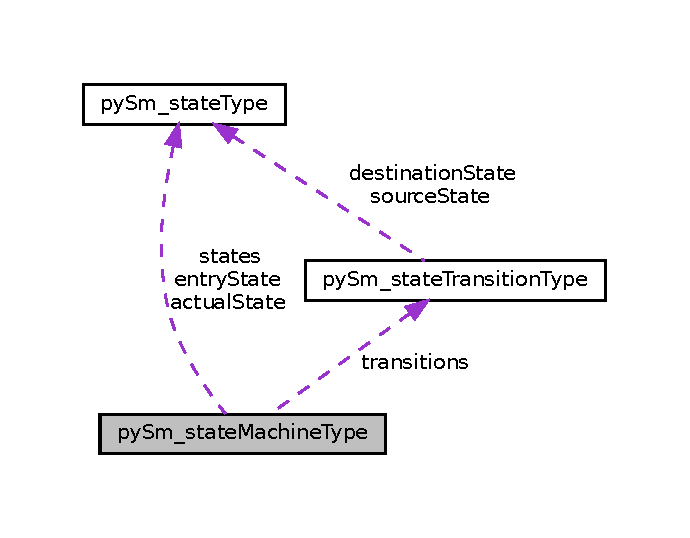
\includegraphics[width=331pt]{structpySm__stateMachineType__coll__graph}
\end{center}
\end{figure}
\subsection*{Data Fields}
\begin{DoxyCompactItemize}
\item 
const \hyperlink{structpySm__stateType}{py\+Sm\+\_\+state\+Type} $\ast$ \hyperlink{structpySm__stateMachineType_ac9896d220e5e80df257943742f47f6d0}{entry\+State}
\item 
\hyperlink{structpySm__stateType}{py\+Sm\+\_\+state\+Type} $\ast$ \hyperlink{structpySm__stateMachineType_afff58d3fb0afd9064dfccf4f58cdb8b5}{actual\+State}
\item 
const \hyperlink{structpySm__stateType}{py\+Sm\+\_\+state\+Type} $\ast$$\ast$ \hyperlink{structpySm__stateMachineType_a6b964357abaeecf851825d1203a59582}{states}
\item 
const \hyperlink{PySm__types_8h_a1aff40256c00f194609879f8f6f1e1a1}{py\+Sm\+\_\+uint8} \hyperlink{structpySm__stateMachineType_a8df1d19072975480da4985f99f8ae19e}{number\+Of\+States}
\item 
const \hyperlink{structpySm__stateTransitionType}{py\+Sm\+\_\+state\+Transition\+Type} $\ast$ \hyperlink{structpySm__stateMachineType_a3f35562e1b353b47e2a90a957882a610}{transitions}
\item 
const \hyperlink{PySm__types_8h_a1aff40256c00f194609879f8f6f1e1a1}{py\+Sm\+\_\+uint8} \hyperlink{structpySm__stateMachineType_a3d4035a87cce41845ae138aa2a279e20}{number\+Of\+Transitions}
\item 
\hyperlink{PySm__types_8h_a368133d64634d66410f3fe1343de6ba3}{py\+Sm\+\_\+bool} \hyperlink{structpySm__stateMachineType_a3320131411f6304cba856edbcfedd060}{run\+Entry\+Of\+Initial\+State\+\_\+b}
\item 
const \hyperlink{PySm_8h_acf18fbe39f8464bd70f03199165ef4a2}{py\+Sm\+\_\+state\+Machine\+Reset\+Function} \hyperlink{structpySm__stateMachineType_a37e20b01fecc6d91d5625b0cd10dcfaa}{reset\+Variables}
\end{DoxyCompactItemize}


\subsection{Detailed Description}
Structure defining a state machine. 

A state machine is defined by it\textquotesingle{}s
\begin{DoxyItemize}
\item entry state \hyperlink{structpySm__stateMachineType_ac9896d220e5e80df257943742f47f6d0}{py\+Sm\+\_\+state\+Machine\+Type\+::entry\+State}
\item current active state \hyperlink{structpySm__stateMachineType_afff58d3fb0afd9064dfccf4f58cdb8b5}{py\+Sm\+\_\+state\+Machine\+Type\+::actual\+State}
\item a list of all states, \hyperlink{structpySm__stateMachineType_a6b964357abaeecf851825d1203a59582}{py\+Sm\+\_\+state\+Machine\+Type\+::states} given by an pointer array, pointing to all states of the generated state machine
\item the overall number of all states \hyperlink{structpySm__stateMachineType_a3d4035a87cce41845ae138aa2a279e20}{py\+Sm\+\_\+state\+Machine\+Type\+::number\+Of\+Transitions}
\item all existing transitions of the state machine \hyperlink{structpySm__stateMachineType_a3f35562e1b353b47e2a90a957882a610}{py\+Sm\+\_\+state\+Machine\+Type\+::transitions}, given by an pointer to an array, containing the transitions
\item the overall number of transitions \hyperlink{structpySm__stateMachineType_a3d4035a87cce41845ae138aa2a279e20}{py\+Sm\+\_\+state\+Machine\+Type\+::number\+Of\+Transitions}
\item a flag \hyperlink{structpySm__stateMachineType_a3320131411f6304cba856edbcfedd060}{py\+Sm\+\_\+state\+Machine\+Type\+::run\+Entry\+Of\+Initial\+State\+\_\+b}, enabling the execution of the on\+Entry-\/function of the first, initial state (entry\+State). This flag get\textquotesingle{}s generated as T\+R\+UE when the entry\+State has an on\+Entry statement
\item a function py\+Sm\+\_\+state\+Machine\+Reset\+Function\+::reset\+Variables for resetting the state machine\textquotesingle{}s local variables 
\end{DoxyItemize}

\subsection{Field Documentation}
\mbox{\Hypertarget{structpySm__stateMachineType_afff58d3fb0afd9064dfccf4f58cdb8b5}\label{structpySm__stateMachineType_afff58d3fb0afd9064dfccf4f58cdb8b5}} 
\index{py\+Sm\+\_\+state\+Machine\+Type@{py\+Sm\+\_\+state\+Machine\+Type}!actual\+State@{actual\+State}}
\index{actual\+State@{actual\+State}!py\+Sm\+\_\+state\+Machine\+Type@{py\+Sm\+\_\+state\+Machine\+Type}}
\subsubsection{\texorpdfstring{actual\+State}{actualState}}
{\footnotesize\ttfamily \hyperlink{structpySm__stateType}{py\+Sm\+\_\+state\+Type}$\ast$ py\+Sm\+\_\+state\+Machine\+Type\+::actual\+State}

\mbox{\Hypertarget{structpySm__stateMachineType_ac9896d220e5e80df257943742f47f6d0}\label{structpySm__stateMachineType_ac9896d220e5e80df257943742f47f6d0}} 
\index{py\+Sm\+\_\+state\+Machine\+Type@{py\+Sm\+\_\+state\+Machine\+Type}!entry\+State@{entry\+State}}
\index{entry\+State@{entry\+State}!py\+Sm\+\_\+state\+Machine\+Type@{py\+Sm\+\_\+state\+Machine\+Type}}
\subsubsection{\texorpdfstring{entry\+State}{entryState}}
{\footnotesize\ttfamily const \hyperlink{structpySm__stateType}{py\+Sm\+\_\+state\+Type}$\ast$ py\+Sm\+\_\+state\+Machine\+Type\+::entry\+State}

\mbox{\Hypertarget{structpySm__stateMachineType_a8df1d19072975480da4985f99f8ae19e}\label{structpySm__stateMachineType_a8df1d19072975480da4985f99f8ae19e}} 
\index{py\+Sm\+\_\+state\+Machine\+Type@{py\+Sm\+\_\+state\+Machine\+Type}!number\+Of\+States@{number\+Of\+States}}
\index{number\+Of\+States@{number\+Of\+States}!py\+Sm\+\_\+state\+Machine\+Type@{py\+Sm\+\_\+state\+Machine\+Type}}
\subsubsection{\texorpdfstring{number\+Of\+States}{numberOfStates}}
{\footnotesize\ttfamily const \hyperlink{PySm__types_8h_a1aff40256c00f194609879f8f6f1e1a1}{py\+Sm\+\_\+uint8} py\+Sm\+\_\+state\+Machine\+Type\+::number\+Of\+States}

\mbox{\Hypertarget{structpySm__stateMachineType_a3d4035a87cce41845ae138aa2a279e20}\label{structpySm__stateMachineType_a3d4035a87cce41845ae138aa2a279e20}} 
\index{py\+Sm\+\_\+state\+Machine\+Type@{py\+Sm\+\_\+state\+Machine\+Type}!number\+Of\+Transitions@{number\+Of\+Transitions}}
\index{number\+Of\+Transitions@{number\+Of\+Transitions}!py\+Sm\+\_\+state\+Machine\+Type@{py\+Sm\+\_\+state\+Machine\+Type}}
\subsubsection{\texorpdfstring{number\+Of\+Transitions}{numberOfTransitions}}
{\footnotesize\ttfamily const \hyperlink{PySm__types_8h_a1aff40256c00f194609879f8f6f1e1a1}{py\+Sm\+\_\+uint8} py\+Sm\+\_\+state\+Machine\+Type\+::number\+Of\+Transitions}

\mbox{\Hypertarget{structpySm__stateMachineType_a37e20b01fecc6d91d5625b0cd10dcfaa}\label{structpySm__stateMachineType_a37e20b01fecc6d91d5625b0cd10dcfaa}} 
\index{py\+Sm\+\_\+state\+Machine\+Type@{py\+Sm\+\_\+state\+Machine\+Type}!reset\+Variables@{reset\+Variables}}
\index{reset\+Variables@{reset\+Variables}!py\+Sm\+\_\+state\+Machine\+Type@{py\+Sm\+\_\+state\+Machine\+Type}}
\subsubsection{\texorpdfstring{reset\+Variables}{resetVariables}}
{\footnotesize\ttfamily const \hyperlink{PySm_8h_acf18fbe39f8464bd70f03199165ef4a2}{py\+Sm\+\_\+state\+Machine\+Reset\+Function} py\+Sm\+\_\+state\+Machine\+Type\+::reset\+Variables}

\mbox{\Hypertarget{structpySm__stateMachineType_a3320131411f6304cba856edbcfedd060}\label{structpySm__stateMachineType_a3320131411f6304cba856edbcfedd060}} 
\index{py\+Sm\+\_\+state\+Machine\+Type@{py\+Sm\+\_\+state\+Machine\+Type}!run\+Entry\+Of\+Initial\+State\+\_\+b@{run\+Entry\+Of\+Initial\+State\+\_\+b}}
\index{run\+Entry\+Of\+Initial\+State\+\_\+b@{run\+Entry\+Of\+Initial\+State\+\_\+b}!py\+Sm\+\_\+state\+Machine\+Type@{py\+Sm\+\_\+state\+Machine\+Type}}
\subsubsection{\texorpdfstring{run\+Entry\+Of\+Initial\+State\+\_\+b}{runEntryOfInitialState\_b}}
{\footnotesize\ttfamily \hyperlink{PySm__types_8h_a368133d64634d66410f3fe1343de6ba3}{py\+Sm\+\_\+bool} py\+Sm\+\_\+state\+Machine\+Type\+::run\+Entry\+Of\+Initial\+State\+\_\+b}

\mbox{\Hypertarget{structpySm__stateMachineType_a6b964357abaeecf851825d1203a59582}\label{structpySm__stateMachineType_a6b964357abaeecf851825d1203a59582}} 
\index{py\+Sm\+\_\+state\+Machine\+Type@{py\+Sm\+\_\+state\+Machine\+Type}!states@{states}}
\index{states@{states}!py\+Sm\+\_\+state\+Machine\+Type@{py\+Sm\+\_\+state\+Machine\+Type}}
\subsubsection{\texorpdfstring{states}{states}}
{\footnotesize\ttfamily const \hyperlink{structpySm__stateType}{py\+Sm\+\_\+state\+Type}$\ast$$\ast$ py\+Sm\+\_\+state\+Machine\+Type\+::states}

\mbox{\Hypertarget{structpySm__stateMachineType_a3f35562e1b353b47e2a90a957882a610}\label{structpySm__stateMachineType_a3f35562e1b353b47e2a90a957882a610}} 
\index{py\+Sm\+\_\+state\+Machine\+Type@{py\+Sm\+\_\+state\+Machine\+Type}!transitions@{transitions}}
\index{transitions@{transitions}!py\+Sm\+\_\+state\+Machine\+Type@{py\+Sm\+\_\+state\+Machine\+Type}}
\subsubsection{\texorpdfstring{transitions}{transitions}}
{\footnotesize\ttfamily const \hyperlink{structpySm__stateTransitionType}{py\+Sm\+\_\+state\+Transition\+Type}$\ast$ py\+Sm\+\_\+state\+Machine\+Type\+::transitions}



The documentation for this struct was generated from the following file\+:\begin{DoxyCompactItemize}
\item 
L\+I\+B/\hyperlink{PySm_8h}{Py\+Sm.\+h}\end{DoxyCompactItemize}

\hypertarget{structpySm__stateTransitionType}{}\section{py\+Sm\+\_\+state\+Transition\+Type Struct Reference}
\label{structpySm__stateTransitionType}\index{py\+Sm\+\_\+state\+Transition\+Type@{py\+Sm\+\_\+state\+Transition\+Type}}


Structure defining a state transition.  




{\ttfamily \#include $<$Py\+Sm.\+h$>$}



Collaboration diagram for py\+Sm\+\_\+state\+Transition\+Type\+:\nopagebreak
\begin{figure}[H]
\begin{center}
\leavevmode
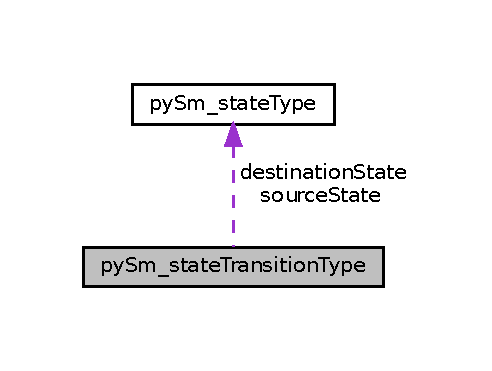
\includegraphics[width=236pt]{structpySm__stateTransitionType__coll__graph}
\end{center}
\end{figure}
\subsection*{Data Fields}
\begin{DoxyCompactItemize}
\item 
const \hyperlink{structpySm__stateType}{py\+Sm\+\_\+state\+Type} $\ast$ \hyperlink{structpySm__stateTransitionType_adb9a41fd9d60f064fabaa74ef2698bd7}{source\+State}
\item 
const \hyperlink{structpySm__stateType}{py\+Sm\+\_\+state\+Type} $\ast$ \hyperlink{structpySm__stateTransitionType_aeff05523d3e91571e745460314e46116}{destination\+State}
\item 
const \hyperlink{PySm_8h_aeedbab67e9dba20efba287fbe3515e43}{py\+Sm\+\_\+transition\+Test\+Function} \hyperlink{structpySm__stateTransitionType_ab3a3cb53af27cfedcc63edb36d5f7639}{transition\+Test}
\item 
const \hyperlink{PySm_8h_ae3950be0321f85684919c1c5e0c3fba1}{py\+Sm\+\_\+transition\+Priority\+Type} \hyperlink{structpySm__stateTransitionType_a0c95a5a437e65155d1100d3016f9575f}{transition\+Priority}
\item 
const \hyperlink{PySm_8h_ac67ca0ce02947dc3f915629091327717}{py\+Sm\+\_\+transition\+Action\+Function} \hyperlink{structpySm__stateTransitionType_a02fc12242851c7d129808a4e81cf1b78}{transition\+Action}
\end{DoxyCompactItemize}


\subsection{Detailed Description}
Structure defining a state transition. 

A state transition is defined by it\textquotesingle{}s
\begin{DoxyItemize}
\item source \hyperlink{structpySm__stateTransitionType_adb9a41fd9d60f064fabaa74ef2698bd7}{py\+Sm\+\_\+state\+Transition\+Type\+::source\+State} and
\item destination state \hyperlink{structpySm__stateTransitionType_aeff05523d3e91571e745460314e46116}{py\+Sm\+\_\+state\+Transition\+Type\+::destination\+State} ,
\item it\textquotesingle{}s transition condition py\+Sm\+\_\+\+State\+Transition\+Type\+::transition\+Test (given by the transition test function) ,
\item the transitions priority \hyperlink{structpySm__stateTransitionType_a0c95a5a437e65155d1100d3016f9575f}{py\+Sm\+\_\+state\+Transition\+Type\+::transition\+Priority}
\item and actions to be performed, if an transition has been triggered, given by the transition action function \hyperlink{structpySm__stateTransitionType_a02fc12242851c7d129808a4e81cf1b78}{py\+Sm\+\_\+state\+Transition\+Type\+::transition\+Action} 
\end{DoxyItemize}

\subsection{Field Documentation}
\mbox{\Hypertarget{structpySm__stateTransitionType_aeff05523d3e91571e745460314e46116}\label{structpySm__stateTransitionType_aeff05523d3e91571e745460314e46116}} 
\index{py\+Sm\+\_\+state\+Transition\+Type@{py\+Sm\+\_\+state\+Transition\+Type}!destination\+State@{destination\+State}}
\index{destination\+State@{destination\+State}!py\+Sm\+\_\+state\+Transition\+Type@{py\+Sm\+\_\+state\+Transition\+Type}}
\subsubsection{\texorpdfstring{destination\+State}{destinationState}}
{\footnotesize\ttfamily const \hyperlink{structpySm__stateType}{py\+Sm\+\_\+state\+Type}$\ast$ py\+Sm\+\_\+state\+Transition\+Type\+::destination\+State}

\mbox{\Hypertarget{structpySm__stateTransitionType_adb9a41fd9d60f064fabaa74ef2698bd7}\label{structpySm__stateTransitionType_adb9a41fd9d60f064fabaa74ef2698bd7}} 
\index{py\+Sm\+\_\+state\+Transition\+Type@{py\+Sm\+\_\+state\+Transition\+Type}!source\+State@{source\+State}}
\index{source\+State@{source\+State}!py\+Sm\+\_\+state\+Transition\+Type@{py\+Sm\+\_\+state\+Transition\+Type}}
\subsubsection{\texorpdfstring{source\+State}{sourceState}}
{\footnotesize\ttfamily const \hyperlink{structpySm__stateType}{py\+Sm\+\_\+state\+Type}$\ast$ py\+Sm\+\_\+state\+Transition\+Type\+::source\+State}

\mbox{\Hypertarget{structpySm__stateTransitionType_a02fc12242851c7d129808a4e81cf1b78}\label{structpySm__stateTransitionType_a02fc12242851c7d129808a4e81cf1b78}} 
\index{py\+Sm\+\_\+state\+Transition\+Type@{py\+Sm\+\_\+state\+Transition\+Type}!transition\+Action@{transition\+Action}}
\index{transition\+Action@{transition\+Action}!py\+Sm\+\_\+state\+Transition\+Type@{py\+Sm\+\_\+state\+Transition\+Type}}
\subsubsection{\texorpdfstring{transition\+Action}{transitionAction}}
{\footnotesize\ttfamily const \hyperlink{PySm_8h_ac67ca0ce02947dc3f915629091327717}{py\+Sm\+\_\+transition\+Action\+Function} py\+Sm\+\_\+state\+Transition\+Type\+::transition\+Action}

\mbox{\Hypertarget{structpySm__stateTransitionType_a0c95a5a437e65155d1100d3016f9575f}\label{structpySm__stateTransitionType_a0c95a5a437e65155d1100d3016f9575f}} 
\index{py\+Sm\+\_\+state\+Transition\+Type@{py\+Sm\+\_\+state\+Transition\+Type}!transition\+Priority@{transition\+Priority}}
\index{transition\+Priority@{transition\+Priority}!py\+Sm\+\_\+state\+Transition\+Type@{py\+Sm\+\_\+state\+Transition\+Type}}
\subsubsection{\texorpdfstring{transition\+Priority}{transitionPriority}}
{\footnotesize\ttfamily const \hyperlink{PySm_8h_ae3950be0321f85684919c1c5e0c3fba1}{py\+Sm\+\_\+transition\+Priority\+Type} py\+Sm\+\_\+state\+Transition\+Type\+::transition\+Priority}

\mbox{\Hypertarget{structpySm__stateTransitionType_ab3a3cb53af27cfedcc63edb36d5f7639}\label{structpySm__stateTransitionType_ab3a3cb53af27cfedcc63edb36d5f7639}} 
\index{py\+Sm\+\_\+state\+Transition\+Type@{py\+Sm\+\_\+state\+Transition\+Type}!transition\+Test@{transition\+Test}}
\index{transition\+Test@{transition\+Test}!py\+Sm\+\_\+state\+Transition\+Type@{py\+Sm\+\_\+state\+Transition\+Type}}
\subsubsection{\texorpdfstring{transition\+Test}{transitionTest}}
{\footnotesize\ttfamily const \hyperlink{PySm_8h_aeedbab67e9dba20efba287fbe3515e43}{py\+Sm\+\_\+transition\+Test\+Function} py\+Sm\+\_\+state\+Transition\+Type\+::transition\+Test}



The documentation for this struct was generated from the following file\+:\begin{DoxyCompactItemize}
\item 
L\+I\+B/\hyperlink{PySm_8h}{Py\+Sm.\+h}\end{DoxyCompactItemize}

\hypertarget{structpySm__stateType}{}\section{py\+Sm\+\_\+state\+Type Struct Reference}
\label{structpySm__stateType}\index{py\+Sm\+\_\+state\+Type@{py\+Sm\+\_\+state\+Type}}


Structure defining a state.  




{\ttfamily \#include $<$Py\+Sm.\+h$>$}

\subsection*{Data Fields}
\begin{DoxyCompactItemize}
\item 
const \hyperlink{PySm_8h_a4f768845ccbe1d4a74cabced29df0c9f}{py\+Sm\+\_\+state\+Function} \hyperlink{structpySm__stateType_acd3c4f8cca7d7792fee332c61419553f}{on\+Entry\+State}
\item 
const \hyperlink{PySm_8h_a4f768845ccbe1d4a74cabced29df0c9f}{py\+Sm\+\_\+state\+Function} \hyperlink{structpySm__stateType_a189eccdfa6bcafd4964b27834edb38c8}{on\+State}
\item 
const \hyperlink{PySm_8h_a4f768845ccbe1d4a74cabced29df0c9f}{py\+Sm\+\_\+state\+Function} \hyperlink{structpySm__stateType_aba503ee3ae11c3303088c94fa30d30d0}{on\+Exit\+State}
\end{DoxyCompactItemize}


\subsection{Detailed Description}
Structure defining a state. 

A state is defined by it\textquotesingle{}s
\begin{DoxyItemize}
\item entry function Py\+Sm\+\_\+\+State\+Type\+::on\+Entry\+State
\item during (state main function) Py\+Sm\+\_\+\+State\+Type\+::on\+State
\item exit function Py\+Sm\+\_\+\+State\+Type\+::on\+Exit\+State. Each of these functions can be generated as N\+U\+L\+L\+\_\+\+P\+TR, if not needed 
\end{DoxyItemize}

\subsection{Field Documentation}
\mbox{\Hypertarget{structpySm__stateType_acd3c4f8cca7d7792fee332c61419553f}\label{structpySm__stateType_acd3c4f8cca7d7792fee332c61419553f}} 
\index{py\+Sm\+\_\+state\+Type@{py\+Sm\+\_\+state\+Type}!on\+Entry\+State@{on\+Entry\+State}}
\index{on\+Entry\+State@{on\+Entry\+State}!py\+Sm\+\_\+state\+Type@{py\+Sm\+\_\+state\+Type}}
\subsubsection{\texorpdfstring{on\+Entry\+State}{onEntryState}}
{\footnotesize\ttfamily const \hyperlink{PySm_8h_a4f768845ccbe1d4a74cabced29df0c9f}{py\+Sm\+\_\+state\+Function} py\+Sm\+\_\+state\+Type\+::on\+Entry\+State}

On\+Entry\+State-\/function, if needed. \mbox{\Hypertarget{structpySm__stateType_aba503ee3ae11c3303088c94fa30d30d0}\label{structpySm__stateType_aba503ee3ae11c3303088c94fa30d30d0}} 
\index{py\+Sm\+\_\+state\+Type@{py\+Sm\+\_\+state\+Type}!on\+Exit\+State@{on\+Exit\+State}}
\index{on\+Exit\+State@{on\+Exit\+State}!py\+Sm\+\_\+state\+Type@{py\+Sm\+\_\+state\+Type}}
\subsubsection{\texorpdfstring{on\+Exit\+State}{onExitState}}
{\footnotesize\ttfamily const \hyperlink{PySm_8h_a4f768845ccbe1d4a74cabced29df0c9f}{py\+Sm\+\_\+state\+Function} py\+Sm\+\_\+state\+Type\+::on\+Exit\+State}

On\+Exit\+State-\/function, if needed. \mbox{\Hypertarget{structpySm__stateType_a189eccdfa6bcafd4964b27834edb38c8}\label{structpySm__stateType_a189eccdfa6bcafd4964b27834edb38c8}} 
\index{py\+Sm\+\_\+state\+Type@{py\+Sm\+\_\+state\+Type}!on\+State@{on\+State}}
\index{on\+State@{on\+State}!py\+Sm\+\_\+state\+Type@{py\+Sm\+\_\+state\+Type}}
\subsubsection{\texorpdfstring{on\+State}{onState}}
{\footnotesize\ttfamily const \hyperlink{PySm_8h_a4f768845ccbe1d4a74cabced29df0c9f}{py\+Sm\+\_\+state\+Function} py\+Sm\+\_\+state\+Type\+::on\+State}

On\+During\+State-\/function, if needed. 

The documentation for this struct was generated from the following file\+:\begin{DoxyCompactItemize}
\item 
L\+I\+B/\hyperlink{PySm_8h}{Py\+Sm.\+h}\end{DoxyCompactItemize}

\chapter{File Documentation}
\hypertarget{PySm_8d}{}\section{Debug/\+L\+I\+B/\+Py\+Sm.d File Reference}
\label{PySm_8d}\index{Debug/\+L\+I\+B/\+Py\+Sm.\+d@{Debug/\+L\+I\+B/\+Py\+Sm.\+d}}

\hypertarget{main_8d}{}\section{Debug/main.d File Reference}
\label{main_8d}\index{Debug/main.\+d@{Debug/main.\+d}}

\hypertarget{DevCoffee_8d}{}\section{Debug/\+S\+W\+C/gen\+S\+M/\+Dev\+Coffee.d File Reference}
\label{DevCoffee_8d}\index{Debug/\+S\+W\+C/gen\+S\+M/\+Dev\+Coffee.\+d@{Debug/\+S\+W\+C/gen\+S\+M/\+Dev\+Coffee.\+d}}

\hypertarget{SimpleEx_8d}{}\section{Debug/\+S\+W\+C/gen\+S\+M/\+Simple\+Ex.d File Reference}
\label{SimpleEx_8d}\index{Debug/\+S\+W\+C/gen\+S\+M/\+Simple\+Ex.\+d@{Debug/\+S\+W\+C/gen\+S\+M/\+Simple\+Ex.\+d}}

\hypertarget{Swc_8d}{}\section{Debug/\+S\+W\+C/\+Swc.d File Reference}
\label{Swc_8d}\index{Debug/\+S\+W\+C/\+Swc.\+d@{Debug/\+S\+W\+C/\+Swc.\+d}}

\hypertarget{PySm_8c}{}\section{L\+I\+B/\+Py\+Sm.c File Reference}
\label{PySm_8c}\index{L\+I\+B/\+Py\+Sm.\+c@{L\+I\+B/\+Py\+Sm.\+c}}


File containing the main implementation of the py\+SM A\+PI and internal functions.  


{\ttfamily \#include \char`\"{}Py\+Sm.\+h\char`\"{}}\newline
Include dependency graph for Py\+Sm.\+c\+:\nopagebreak
\begin{figure}[H]
\begin{center}
\leavevmode
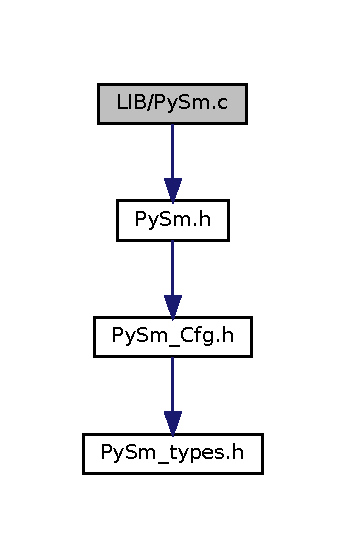
\includegraphics[width=166pt]{PySm_8c__incl}
\end{center}
\end{figure}
\subsection*{Functions}
\begin{DoxyCompactItemize}
\item 
static \hyperlink{PySm_8h_a1bd760b7300136bf7e0bd7b9e3a126ff}{py\+Sm\+\_\+return\+Type} \hyperlink{PySm_8c_ae2ee66c8ec089cbd4bf9bb64b876241d}{Py\+Sm\+\_\+check\+State} (const \hyperlink{structpySm__stateMachineType}{py\+Sm\+\_\+state\+Machine\+Type} $\ast$state\+Machine, const \hyperlink{structpySm__stateType}{py\+Sm\+\_\+state\+Type} $\ast$state\+To\+Check)
\begin{DoxyCompactList}\small\item\em Checks a state of a given state machine. \end{DoxyCompactList}\item 
\hyperlink{PySm_8h_a1bd760b7300136bf7e0bd7b9e3a126ff}{py\+Sm\+\_\+return\+Type} \hyperlink{PySm_8c_ada20de83c4f6830d43987e68c86ba8f5}{Py\+Sm\+\_\+run\+State\+Machine} (\hyperlink{structpySm__stateMachineType}{py\+Sm\+\_\+state\+Machine\+Type} $\ast$state\+Machine)
\begin{DoxyCompactList}\small\item\em Runs the given state machine. \end{DoxyCompactList}\item 
\hyperlink{PySm_8h_a1bd760b7300136bf7e0bd7b9e3a126ff}{py\+Sm\+\_\+return\+Type} \hyperlink{PySm_8c_a78b95f410fec8c7bf67ee6c38631bea7}{Py\+Sm\+\_\+reset\+State\+Machine} (\hyperlink{structpySm__stateMachineType}{py\+Sm\+\_\+state\+Machine\+Type} $\ast$state\+Machine)
\begin{DoxyCompactList}\small\item\em Resets the given state machine. \end{DoxyCompactList}\end{DoxyCompactItemize}


\subsection{Detailed Description}
File containing the main implementation of the py\+SM A\+PI and internal functions. 

\begin{DoxyAuthor}{Author}
Markus Burger 
\end{DoxyAuthor}
\begin{DoxyDate}{Date}
2017-\/09-\/11 
\end{DoxyDate}


\subsection{Function Documentation}
\mbox{\Hypertarget{PySm_8c_ae2ee66c8ec089cbd4bf9bb64b876241d}\label{PySm_8c_ae2ee66c8ec089cbd4bf9bb64b876241d}} 
\index{Py\+Sm.\+c@{Py\+Sm.\+c}!Py\+Sm\+\_\+check\+State@{Py\+Sm\+\_\+check\+State}}
\index{Py\+Sm\+\_\+check\+State@{Py\+Sm\+\_\+check\+State}!Py\+Sm.\+c@{Py\+Sm.\+c}}
\subsubsection{\texorpdfstring{Py\+Sm\+\_\+check\+State()}{PySm\_checkState()}}
{\footnotesize\ttfamily static \hyperlink{PySm_8h_a1bd760b7300136bf7e0bd7b9e3a126ff}{py\+Sm\+\_\+return\+Type} Py\+Sm\+\_\+check\+State (\begin{DoxyParamCaption}\item[{const \hyperlink{structpySm__stateMachineType}{py\+Sm\+\_\+state\+Machine\+Type} $\ast$}]{state\+Machine,  }\item[{const \hyperlink{structpySm__stateType}{py\+Sm\+\_\+state\+Type} $\ast$}]{state\+To\+Check }\end{DoxyParamCaption})\hspace{0.3cm}{\ttfamily [static]}}



Checks a state of a given state machine. 

Checks, if a given state exists in a given state machine 
\begin{DoxyCode}
\hyperlink{PySm_8h_a1bd760b7300136bf7e0bd7b9e3a126ff}{pySm\_returnType} out = pySm\_checkState(&stateMachine, &stateToCheck);
\end{DoxyCode}
 
\begin{DoxyParams}{Parameters}
{\em state\+Machine} & State machine object \\
\hline
{\em state\+To\+Check} & State to check if existing in {\ttfamily state\+Machine} \\
\hline
\end{DoxyParams}
\begin{DoxyReturn}{Returns}
Returns either P\+Y\+S\+M\+\_\+\+E\+\_\+\+U\+N\+K\+N\+O\+W\+N\+\_\+\+S\+T\+A\+TE when the given state doesn\textquotesingle{}t exist in {\ttfamily state\+Machine} or P\+Y\+S\+M\+\_\+\+E\+\_\+\+OK 
\end{DoxyReturn}
\mbox{\Hypertarget{PySm_8c_a78b95f410fec8c7bf67ee6c38631bea7}\label{PySm_8c_a78b95f410fec8c7bf67ee6c38631bea7}} 
\index{Py\+Sm.\+c@{Py\+Sm.\+c}!Py\+Sm\+\_\+reset\+State\+Machine@{Py\+Sm\+\_\+reset\+State\+Machine}}
\index{Py\+Sm\+\_\+reset\+State\+Machine@{Py\+Sm\+\_\+reset\+State\+Machine}!Py\+Sm.\+c@{Py\+Sm.\+c}}
\subsubsection{\texorpdfstring{Py\+Sm\+\_\+reset\+State\+Machine()}{PySm\_resetStateMachine()}}
{\footnotesize\ttfamily \hyperlink{PySm_8h_a1bd760b7300136bf7e0bd7b9e3a126ff}{py\+Sm\+\_\+return\+Type} Py\+Sm\+\_\+reset\+State\+Machine (\begin{DoxyParamCaption}\item[{\hyperlink{structpySm__stateMachineType}{py\+Sm\+\_\+state\+Machine\+Type} $\ast$}]{state\+Machine }\end{DoxyParamCaption})}



Resets the given state machine. 

Resets the given state machine back to initial state and resets the state machine\textquotesingle{}s local variables back to their initial values 
\begin{DoxyCode}
\hyperlink{PySm_8h_a1bd760b7300136bf7e0bd7b9e3a126ff}{pySm\_returnType} out = pySm\_resetStateMachine(&stateMachine);
\end{DoxyCode}
 
\begin{DoxyParams}{Parameters}
{\em state\+Machine} & State machine object to reset \\
\hline
\end{DoxyParams}
\begin{DoxyReturn}{Returns}
Returns either P\+Y\+S\+M\+\_\+\+I\+N\+V\+A\+L\+I\+D\+\_\+\+M\+A\+C\+H\+I\+NE when an invalid state\+Machine has been given or P\+Y\+S\+M\+\_\+\+E\+\_\+\+OK 
\end{DoxyReturn}
Here is the call graph for this function\+:\nopagebreak
\begin{figure}[H]
\begin{center}
\leavevmode
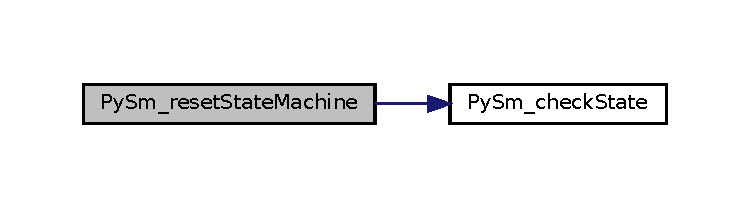
\includegraphics[width=350pt]{PySm_8c_a78b95f410fec8c7bf67ee6c38631bea7_cgraph}
\end{center}
\end{figure}
\mbox{\Hypertarget{PySm_8c_ada20de83c4f6830d43987e68c86ba8f5}\label{PySm_8c_ada20de83c4f6830d43987e68c86ba8f5}} 
\index{Py\+Sm.\+c@{Py\+Sm.\+c}!Py\+Sm\+\_\+run\+State\+Machine@{Py\+Sm\+\_\+run\+State\+Machine}}
\index{Py\+Sm\+\_\+run\+State\+Machine@{Py\+Sm\+\_\+run\+State\+Machine}!Py\+Sm.\+c@{Py\+Sm.\+c}}
\subsubsection{\texorpdfstring{Py\+Sm\+\_\+run\+State\+Machine()}{PySm\_runStateMachine()}}
{\footnotesize\ttfamily \hyperlink{PySm_8h_a1bd760b7300136bf7e0bd7b9e3a126ff}{py\+Sm\+\_\+return\+Type} Py\+Sm\+\_\+run\+State\+Machine (\begin{DoxyParamCaption}\item[{\hyperlink{structpySm__stateMachineType}{py\+Sm\+\_\+state\+Machine\+Type} $\ast$}]{state\+Machine }\end{DoxyParamCaption})}



Runs the given state machine. 

Executes the given state machine 
\begin{DoxyCode}
\hyperlink{PySm_8h_a1bd760b7300136bf7e0bd7b9e3a126ff}{pySm\_returnType} out = pySm\_runStateMachine(&stateMachine);
\end{DoxyCode}
 
\begin{DoxyParams}{Parameters}
{\em state\+Machine} & State machine object to run \\
\hline
\end{DoxyParams}
\begin{DoxyReturn}{Returns}
Returns either P\+Y\+S\+M\+\_\+\+I\+N\+V\+A\+L\+I\+D\+\_\+\+M\+A\+C\+H\+I\+NE when an invalid statemachine has been given or P\+Y\+S\+M\+\_\+\+E\+\_\+\+OK 
\end{DoxyReturn}
Here is the call graph for this function\+:\nopagebreak
\begin{figure}[H]
\begin{center}
\leavevmode
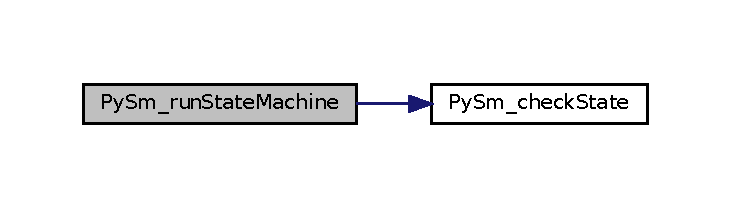
\includegraphics[width=350pt]{PySm_8c_ada20de83c4f6830d43987e68c86ba8f5_cgraph}
\end{center}
\end{figure}

\hypertarget{PySm_8h}{}\section{L\+I\+B/\+Py\+Sm.h File Reference}
\label{PySm_8h}\index{L\+I\+B/\+Py\+Sm.\+h@{L\+I\+B/\+Py\+Sm.\+h}}


File containing typedefs and extern callable function declarations.  


{\ttfamily \#include \char`\"{}Py\+Sm\+\_\+\+Cfg.\+h\char`\"{}}\newline
Include dependency graph for Py\+Sm.\+h\+:\nopagebreak
\begin{figure}[H]
\begin{center}
\leavevmode
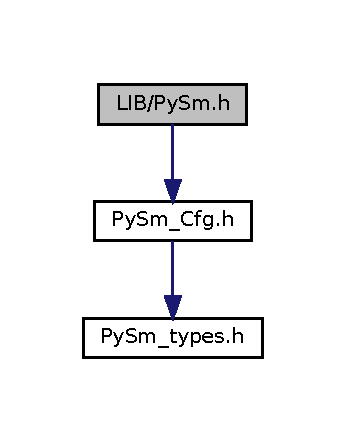
\includegraphics[width=166pt]{PySm_8h__incl}
\end{center}
\end{figure}
This graph shows which files directly or indirectly include this file\+:
\nopagebreak
\begin{figure}[H]
\begin{center}
\leavevmode
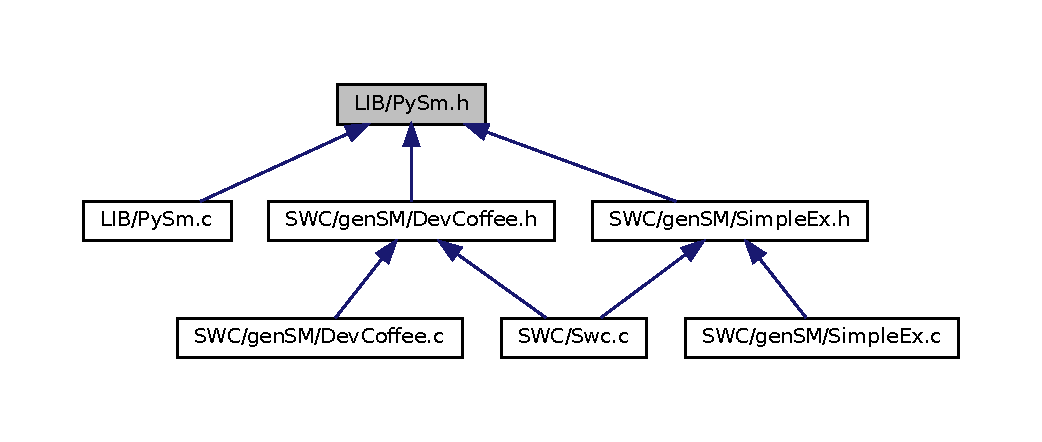
\includegraphics[width=350pt]{PySm_8h__dep__incl}
\end{center}
\end{figure}
\subsection*{Data Structures}
\begin{DoxyCompactItemize}
\item 
struct \hyperlink{structpySm__stateType}{py\+Sm\+\_\+state\+Type}
\begin{DoxyCompactList}\small\item\em Structure defining a state. \end{DoxyCompactList}\item 
struct \hyperlink{structpySm__stateTransitionType}{py\+Sm\+\_\+state\+Transition\+Type}
\begin{DoxyCompactList}\small\item\em Structure defining a state transition. \end{DoxyCompactList}\item 
struct \hyperlink{structpySm__stateMachineType}{py\+Sm\+\_\+state\+Machine\+Type}
\begin{DoxyCompactList}\small\item\em Structure defining a state machine. \end{DoxyCompactList}\end{DoxyCompactItemize}
\subsection*{Typedefs}
\begin{DoxyCompactItemize}
\item 
typedef void($\ast$ \hyperlink{PySm_8h_a4f768845ccbe1d4a74cabced29df0c9f}{py\+Sm\+\_\+state\+Function}) (void)
\begin{DoxyCompactList}\small\item\em Function pointer definition for state functions. \end{DoxyCompactList}\item 
typedef void($\ast$ \hyperlink{PySm_8h_acf18fbe39f8464bd70f03199165ef4a2}{py\+Sm\+\_\+state\+Machine\+Reset\+Function}) (void)
\begin{DoxyCompactList}\small\item\em Function pointer definition for state machine reset functions. \end{DoxyCompactList}\item 
typedef void($\ast$ \hyperlink{PySm_8h_ac67ca0ce02947dc3f915629091327717}{py\+Sm\+\_\+transition\+Action\+Function}) (void)
\begin{DoxyCompactList}\small\item\em Function pointer definition for state transition functions. \end{DoxyCompactList}\item 
typedef \hyperlink{PySm__types_8h_a368133d64634d66410f3fe1343de6ba3}{py\+Sm\+\_\+bool}($\ast$ \hyperlink{PySm_8h_aeedbab67e9dba20efba287fbe3515e43}{py\+Sm\+\_\+transition\+Test\+Function}) (void)
\begin{DoxyCompactList}\small\item\em Function pointer definition for state transition test functions. \end{DoxyCompactList}\item 
typedef \hyperlink{PySm__types_8h_a1aff40256c00f194609879f8f6f1e1a1}{py\+Sm\+\_\+uint8} \hyperlink{PySm_8h_ae3950be0321f85684919c1c5e0c3fba1}{py\+Sm\+\_\+transition\+Priority\+Type}
\begin{DoxyCompactList}\small\item\em Type for transition priorities. \end{DoxyCompactList}\end{DoxyCompactItemize}
\subsection*{Enumerations}
\begin{DoxyCompactItemize}
\item 
enum \hyperlink{PySm_8h_a1bd760b7300136bf7e0bd7b9e3a126ff}{py\+Sm\+\_\+return\+Type} \{ \hyperlink{PySm_8h_a1bd760b7300136bf7e0bd7b9e3a126ffac9cd51f7be16280426493d5285bad96a}{P\+Y\+S\+M\+\_\+\+E\+\_\+\+OK} = 0u, 
\hyperlink{PySm_8h_a1bd760b7300136bf7e0bd7b9e3a126ffab6285a1e8c2112c1d895805a6da392ed}{P\+Y\+S\+M\+\_\+\+E\+\_\+\+U\+N\+K\+N\+O\+W\+N\+\_\+\+S\+T\+A\+TE}, 
\hyperlink{PySm_8h_a1bd760b7300136bf7e0bd7b9e3a126ffa15946f57e2fbab7637db1bcd3105c5c7}{P\+Y\+S\+M\+\_\+\+E\+\_\+\+U\+N\+K\+N\+O\+W\+N\+\_\+\+T\+R\+A\+N\+S\+I\+T\+I\+ON}, 
\hyperlink{PySm_8h_a1bd760b7300136bf7e0bd7b9e3a126ffa23b317ace925bfad0ac732a6f3f1a810}{P\+Y\+S\+M\+\_\+\+I\+N\+V\+A\+L\+I\+D\+\_\+\+M\+A\+C\+H\+I\+NE}
 \}\begin{DoxyCompactList}\small\item\em Return type for the py\+SM librarie\textquotesingle{}s A\+PI functions. \end{DoxyCompactList}
\end{DoxyCompactItemize}
\subsection*{Functions}
\begin{DoxyCompactItemize}
\item 
\hyperlink{PySm_8h_a1bd760b7300136bf7e0bd7b9e3a126ff}{py\+Sm\+\_\+return\+Type} \hyperlink{PySm_8h_ada20de83c4f6830d43987e68c86ba8f5}{Py\+Sm\+\_\+run\+State\+Machine} (\hyperlink{structpySm__stateMachineType}{py\+Sm\+\_\+state\+Machine\+Type} $\ast$state\+Machine)
\begin{DoxyCompactList}\small\item\em Runs the given state machine. \end{DoxyCompactList}\item 
\hyperlink{PySm_8h_a1bd760b7300136bf7e0bd7b9e3a126ff}{py\+Sm\+\_\+return\+Type} \hyperlink{PySm_8h_a78b95f410fec8c7bf67ee6c38631bea7}{Py\+Sm\+\_\+reset\+State\+Machine} (\hyperlink{structpySm__stateMachineType}{py\+Sm\+\_\+state\+Machine\+Type} $\ast$state\+Machine)
\begin{DoxyCompactList}\small\item\em Resets the given state machine. \end{DoxyCompactList}\end{DoxyCompactItemize}


\subsection{Detailed Description}
File containing typedefs and extern callable function declarations. 

\begin{DoxyAuthor}{Author}
Markus Burger 
\end{DoxyAuthor}
\begin{DoxyDate}{Date}
2017-\/09-\/11 
\end{DoxyDate}


\subsection{Typedef Documentation}
\mbox{\Hypertarget{PySm_8h_a4f768845ccbe1d4a74cabced29df0c9f}\label{PySm_8h_a4f768845ccbe1d4a74cabced29df0c9f}} 
\index{Py\+Sm.\+h@{Py\+Sm.\+h}!py\+Sm\+\_\+state\+Function@{py\+Sm\+\_\+state\+Function}}
\index{py\+Sm\+\_\+state\+Function@{py\+Sm\+\_\+state\+Function}!Py\+Sm.\+h@{Py\+Sm.\+h}}
\subsubsection{\texorpdfstring{py\+Sm\+\_\+state\+Function}{pySm\_stateFunction}}
{\footnotesize\ttfamily typedef void($\ast$ py\+Sm\+\_\+state\+Function) (void)}



Function pointer definition for state functions. 

\mbox{\Hypertarget{PySm_8h_acf18fbe39f8464bd70f03199165ef4a2}\label{PySm_8h_acf18fbe39f8464bd70f03199165ef4a2}} 
\index{Py\+Sm.\+h@{Py\+Sm.\+h}!py\+Sm\+\_\+state\+Machine\+Reset\+Function@{py\+Sm\+\_\+state\+Machine\+Reset\+Function}}
\index{py\+Sm\+\_\+state\+Machine\+Reset\+Function@{py\+Sm\+\_\+state\+Machine\+Reset\+Function}!Py\+Sm.\+h@{Py\+Sm.\+h}}
\subsubsection{\texorpdfstring{py\+Sm\+\_\+state\+Machine\+Reset\+Function}{pySm\_stateMachineResetFunction}}
{\footnotesize\ttfamily typedef void($\ast$ py\+Sm\+\_\+state\+Machine\+Reset\+Function) (void)}



Function pointer definition for state machine reset functions. 

This function get\textquotesingle{}s generated and is used to reset state machine local internal static variables. This function normally get\textquotesingle{}s called only when resetting a whole state machine by the according A\+PI function. \mbox{\Hypertarget{PySm_8h_ac67ca0ce02947dc3f915629091327717}\label{PySm_8h_ac67ca0ce02947dc3f915629091327717}} 
\index{Py\+Sm.\+h@{Py\+Sm.\+h}!py\+Sm\+\_\+transition\+Action\+Function@{py\+Sm\+\_\+transition\+Action\+Function}}
\index{py\+Sm\+\_\+transition\+Action\+Function@{py\+Sm\+\_\+transition\+Action\+Function}!Py\+Sm.\+h@{Py\+Sm.\+h}}
\subsubsection{\texorpdfstring{py\+Sm\+\_\+transition\+Action\+Function}{pySm\_transitionActionFunction}}
{\footnotesize\ttfamily typedef void($\ast$ py\+Sm\+\_\+transition\+Action\+Function) (void)}



Function pointer definition for state transition functions. 

These functions get called (if generated/needed) to perform given actions when a transition gets triggered and executed. \mbox{\Hypertarget{PySm_8h_ae3950be0321f85684919c1c5e0c3fba1}\label{PySm_8h_ae3950be0321f85684919c1c5e0c3fba1}} 
\index{Py\+Sm.\+h@{Py\+Sm.\+h}!py\+Sm\+\_\+transition\+Priority\+Type@{py\+Sm\+\_\+transition\+Priority\+Type}}
\index{py\+Sm\+\_\+transition\+Priority\+Type@{py\+Sm\+\_\+transition\+Priority\+Type}!Py\+Sm.\+h@{Py\+Sm.\+h}}
\subsubsection{\texorpdfstring{py\+Sm\+\_\+transition\+Priority\+Type}{pySm\_transitionPriorityType}}
{\footnotesize\ttfamily typedef \hyperlink{PySm__types_8h_a1aff40256c00f194609879f8f6f1e1a1}{py\+Sm\+\_\+uint8} \hyperlink{PySm_8h_ae3950be0321f85684919c1c5e0c3fba1}{py\+Sm\+\_\+transition\+Priority\+Type}}



Type for transition priorities. 

\mbox{\Hypertarget{PySm_8h_aeedbab67e9dba20efba287fbe3515e43}\label{PySm_8h_aeedbab67e9dba20efba287fbe3515e43}} 
\index{Py\+Sm.\+h@{Py\+Sm.\+h}!py\+Sm\+\_\+transition\+Test\+Function@{py\+Sm\+\_\+transition\+Test\+Function}}
\index{py\+Sm\+\_\+transition\+Test\+Function@{py\+Sm\+\_\+transition\+Test\+Function}!Py\+Sm.\+h@{Py\+Sm.\+h}}
\subsubsection{\texorpdfstring{py\+Sm\+\_\+transition\+Test\+Function}{pySm\_transitionTestFunction}}
{\footnotesize\ttfamily typedef \hyperlink{PySm__types_8h_a368133d64634d66410f3fe1343de6ba3}{py\+Sm\+\_\+bool}($\ast$ py\+Sm\+\_\+transition\+Test\+Function) (void)}



Function pointer definition for state transition test functions. 

These functions get called to perform the evaluation of the transition condition. 

\subsection{Enumeration Type Documentation}
\mbox{\Hypertarget{PySm_8h_a1bd760b7300136bf7e0bd7b9e3a126ff}\label{PySm_8h_a1bd760b7300136bf7e0bd7b9e3a126ff}} 
\index{Py\+Sm.\+h@{Py\+Sm.\+h}!py\+Sm\+\_\+return\+Type@{py\+Sm\+\_\+return\+Type}}
\index{py\+Sm\+\_\+return\+Type@{py\+Sm\+\_\+return\+Type}!Py\+Sm.\+h@{Py\+Sm.\+h}}
\subsubsection{\texorpdfstring{py\+Sm\+\_\+return\+Type}{pySm\_returnType}}
{\footnotesize\ttfamily enum \hyperlink{PySm_8h_a1bd760b7300136bf7e0bd7b9e3a126ff}{py\+Sm\+\_\+return\+Type}}



Return type for the py\+SM librarie\textquotesingle{}s A\+PI functions. 

\begin{DoxyEnumFields}{Enumerator}
\raisebox{\heightof{T}}[0pt][0pt]{\index{P\+Y\+S\+M\+\_\+\+E\+\_\+\+OK@{P\+Y\+S\+M\+\_\+\+E\+\_\+\+OK}!Py\+Sm.\+h@{Py\+Sm.\+h}}\index{Py\+Sm.\+h@{Py\+Sm.\+h}!P\+Y\+S\+M\+\_\+\+E\+\_\+\+OK@{P\+Y\+S\+M\+\_\+\+E\+\_\+\+OK}}}\mbox{\Hypertarget{PySm_8h_a1bd760b7300136bf7e0bd7b9e3a126ffac9cd51f7be16280426493d5285bad96a}\label{PySm_8h_a1bd760b7300136bf7e0bd7b9e3a126ffac9cd51f7be16280426493d5285bad96a}} 
P\+Y\+S\+M\+\_\+\+E\+\_\+\+OK&\\
\hline

\raisebox{\heightof{T}}[0pt][0pt]{\index{P\+Y\+S\+M\+\_\+\+E\+\_\+\+U\+N\+K\+N\+O\+W\+N\+\_\+\+S\+T\+A\+TE@{P\+Y\+S\+M\+\_\+\+E\+\_\+\+U\+N\+K\+N\+O\+W\+N\+\_\+\+S\+T\+A\+TE}!Py\+Sm.\+h@{Py\+Sm.\+h}}\index{Py\+Sm.\+h@{Py\+Sm.\+h}!P\+Y\+S\+M\+\_\+\+E\+\_\+\+U\+N\+K\+N\+O\+W\+N\+\_\+\+S\+T\+A\+TE@{P\+Y\+S\+M\+\_\+\+E\+\_\+\+U\+N\+K\+N\+O\+W\+N\+\_\+\+S\+T\+A\+TE}}}\mbox{\Hypertarget{PySm_8h_a1bd760b7300136bf7e0bd7b9e3a126ffab6285a1e8c2112c1d895805a6da392ed}\label{PySm_8h_a1bd760b7300136bf7e0bd7b9e3a126ffab6285a1e8c2112c1d895805a6da392ed}} 
P\+Y\+S\+M\+\_\+\+E\+\_\+\+U\+N\+K\+N\+O\+W\+N\+\_\+\+S\+T\+A\+TE&\\
\hline

\raisebox{\heightof{T}}[0pt][0pt]{\index{P\+Y\+S\+M\+\_\+\+E\+\_\+\+U\+N\+K\+N\+O\+W\+N\+\_\+\+T\+R\+A\+N\+S\+I\+T\+I\+ON@{P\+Y\+S\+M\+\_\+\+E\+\_\+\+U\+N\+K\+N\+O\+W\+N\+\_\+\+T\+R\+A\+N\+S\+I\+T\+I\+ON}!Py\+Sm.\+h@{Py\+Sm.\+h}}\index{Py\+Sm.\+h@{Py\+Sm.\+h}!P\+Y\+S\+M\+\_\+\+E\+\_\+\+U\+N\+K\+N\+O\+W\+N\+\_\+\+T\+R\+A\+N\+S\+I\+T\+I\+ON@{P\+Y\+S\+M\+\_\+\+E\+\_\+\+U\+N\+K\+N\+O\+W\+N\+\_\+\+T\+R\+A\+N\+S\+I\+T\+I\+ON}}}\mbox{\Hypertarget{PySm_8h_a1bd760b7300136bf7e0bd7b9e3a126ffa15946f57e2fbab7637db1bcd3105c5c7}\label{PySm_8h_a1bd760b7300136bf7e0bd7b9e3a126ffa15946f57e2fbab7637db1bcd3105c5c7}} 
P\+Y\+S\+M\+\_\+\+E\+\_\+\+U\+N\+K\+N\+O\+W\+N\+\_\+\+T\+R\+A\+N\+S\+I\+T\+I\+ON&\\
\hline

\raisebox{\heightof{T}}[0pt][0pt]{\index{P\+Y\+S\+M\+\_\+\+I\+N\+V\+A\+L\+I\+D\+\_\+\+M\+A\+C\+H\+I\+NE@{P\+Y\+S\+M\+\_\+\+I\+N\+V\+A\+L\+I\+D\+\_\+\+M\+A\+C\+H\+I\+NE}!Py\+Sm.\+h@{Py\+Sm.\+h}}\index{Py\+Sm.\+h@{Py\+Sm.\+h}!P\+Y\+S\+M\+\_\+\+I\+N\+V\+A\+L\+I\+D\+\_\+\+M\+A\+C\+H\+I\+NE@{P\+Y\+S\+M\+\_\+\+I\+N\+V\+A\+L\+I\+D\+\_\+\+M\+A\+C\+H\+I\+NE}}}\mbox{\Hypertarget{PySm_8h_a1bd760b7300136bf7e0bd7b9e3a126ffa23b317ace925bfad0ac732a6f3f1a810}\label{PySm_8h_a1bd760b7300136bf7e0bd7b9e3a126ffa23b317ace925bfad0ac732a6f3f1a810}} 
P\+Y\+S\+M\+\_\+\+I\+N\+V\+A\+L\+I\+D\+\_\+\+M\+A\+C\+H\+I\+NE&\\
\hline

\end{DoxyEnumFields}


\subsection{Function Documentation}
\mbox{\Hypertarget{PySm_8h_a78b95f410fec8c7bf67ee6c38631bea7}\label{PySm_8h_a78b95f410fec8c7bf67ee6c38631bea7}} 
\index{Py\+Sm.\+h@{Py\+Sm.\+h}!Py\+Sm\+\_\+reset\+State\+Machine@{Py\+Sm\+\_\+reset\+State\+Machine}}
\index{Py\+Sm\+\_\+reset\+State\+Machine@{Py\+Sm\+\_\+reset\+State\+Machine}!Py\+Sm.\+h@{Py\+Sm.\+h}}
\subsubsection{\texorpdfstring{Py\+Sm\+\_\+reset\+State\+Machine()}{PySm\_resetStateMachine()}}
{\footnotesize\ttfamily \hyperlink{PySm_8h_a1bd760b7300136bf7e0bd7b9e3a126ff}{py\+Sm\+\_\+return\+Type} Py\+Sm\+\_\+reset\+State\+Machine (\begin{DoxyParamCaption}\item[{\hyperlink{structpySm__stateMachineType}{py\+Sm\+\_\+state\+Machine\+Type} $\ast$}]{state\+Machine }\end{DoxyParamCaption})}



Resets the given state machine. 

Resets the given state machine back to initial state and resets the state machine\textquotesingle{}s local variables back to their initial values 
\begin{DoxyCode}
\hyperlink{PySm_8h_a1bd760b7300136bf7e0bd7b9e3a126ff}{pySm\_returnType} out = pySm\_resetStateMachine(&stateMachine);
\end{DoxyCode}
 
\begin{DoxyParams}{Parameters}
{\em state\+Machine} & State machine object to reset \\
\hline
\end{DoxyParams}
\begin{DoxyReturn}{Returns}
Returns either P\+Y\+S\+M\+\_\+\+I\+N\+V\+A\+L\+I\+D\+\_\+\+M\+A\+C\+H\+I\+NE when an invalid state\+Machine has been given or P\+Y\+S\+M\+\_\+\+E\+\_\+\+OK 
\end{DoxyReturn}
Here is the call graph for this function\+:\nopagebreak
\begin{figure}[H]
\begin{center}
\leavevmode
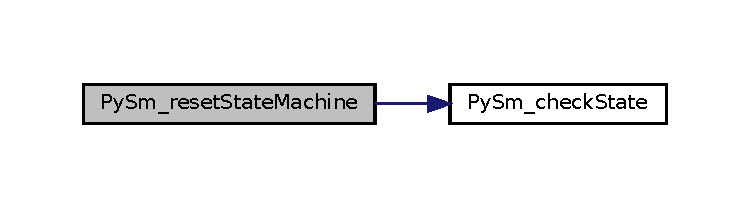
\includegraphics[width=350pt]{PySm_8h_a78b95f410fec8c7bf67ee6c38631bea7_cgraph}
\end{center}
\end{figure}
\mbox{\Hypertarget{PySm_8h_ada20de83c4f6830d43987e68c86ba8f5}\label{PySm_8h_ada20de83c4f6830d43987e68c86ba8f5}} 
\index{Py\+Sm.\+h@{Py\+Sm.\+h}!Py\+Sm\+\_\+run\+State\+Machine@{Py\+Sm\+\_\+run\+State\+Machine}}
\index{Py\+Sm\+\_\+run\+State\+Machine@{Py\+Sm\+\_\+run\+State\+Machine}!Py\+Sm.\+h@{Py\+Sm.\+h}}
\subsubsection{\texorpdfstring{Py\+Sm\+\_\+run\+State\+Machine()}{PySm\_runStateMachine()}}
{\footnotesize\ttfamily \hyperlink{PySm_8h_a1bd760b7300136bf7e0bd7b9e3a126ff}{py\+Sm\+\_\+return\+Type} Py\+Sm\+\_\+run\+State\+Machine (\begin{DoxyParamCaption}\item[{\hyperlink{structpySm__stateMachineType}{py\+Sm\+\_\+state\+Machine\+Type} $\ast$}]{state\+Machine }\end{DoxyParamCaption})}



Runs the given state machine. 

Executes the given state machine 
\begin{DoxyCode}
\hyperlink{PySm_8h_a1bd760b7300136bf7e0bd7b9e3a126ff}{pySm\_returnType} out = pySm\_runStateMachine(&stateMachine);
\end{DoxyCode}
 
\begin{DoxyParams}{Parameters}
{\em state\+Machine} & State machine object to run \\
\hline
\end{DoxyParams}
\begin{DoxyReturn}{Returns}
Returns either P\+Y\+S\+M\+\_\+\+I\+N\+V\+A\+L\+I\+D\+\_\+\+M\+A\+C\+H\+I\+NE when an invalid statemachine has been given or P\+Y\+S\+M\+\_\+\+E\+\_\+\+OK 
\end{DoxyReturn}
Here is the call graph for this function\+:\nopagebreak
\begin{figure}[H]
\begin{center}
\leavevmode
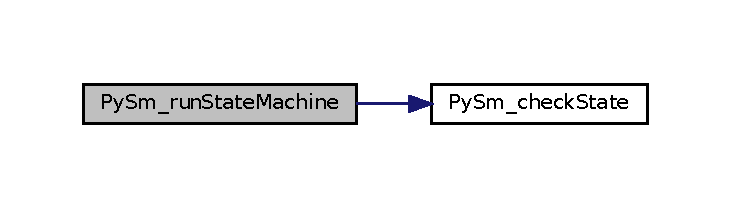
\includegraphics[width=350pt]{PySm_8h_ada20de83c4f6830d43987e68c86ba8f5_cgraph}
\end{center}
\end{figure}

\hypertarget{PySm__Cfg_8h}{}\section{L\+I\+B/\+Py\+Sm\+\_\+\+Cfg.h File Reference}
\label{PySm__Cfg_8h}\index{L\+I\+B/\+Py\+Sm\+\_\+\+Cfg.\+h@{L\+I\+B/\+Py\+Sm\+\_\+\+Cfg.\+h}}


File containing configuration of the py\+SM library.  


{\ttfamily \#include \char`\"{}Py\+Sm\+\_\+types.\+h\char`\"{}}\newline
Include dependency graph for Py\+Sm\+\_\+\+Cfg.\+h\+:\nopagebreak
\begin{figure}[H]
\begin{center}
\leavevmode
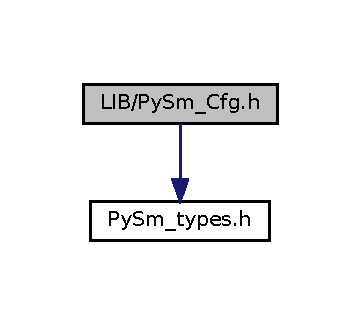
\includegraphics[width=173pt]{PySm__Cfg_8h__incl}
\end{center}
\end{figure}
This graph shows which files directly or indirectly include this file\+:
\nopagebreak
\begin{figure}[H]
\begin{center}
\leavevmode
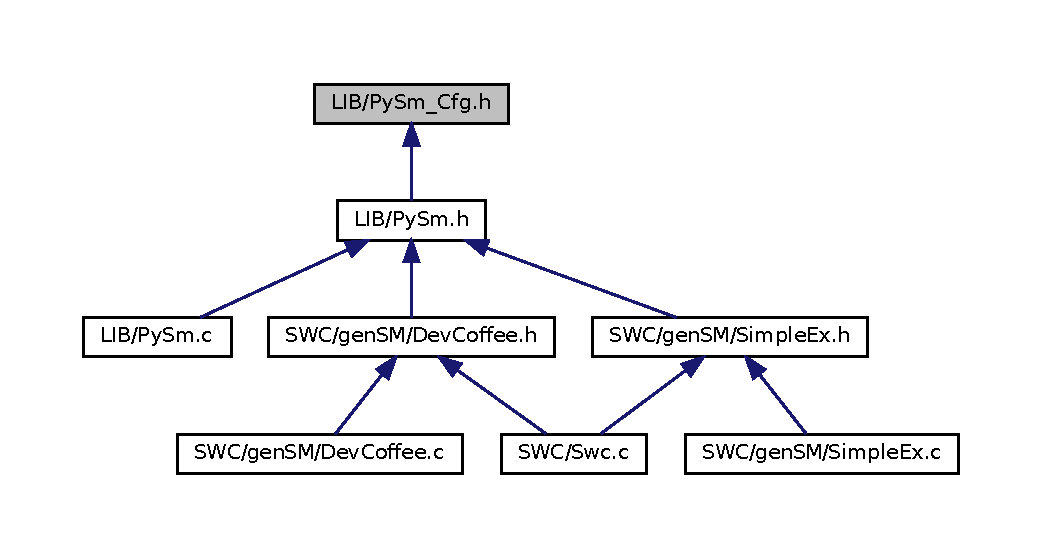
\includegraphics[width=334pt]{PySm__Cfg_8h__dep__incl}
\end{center}
\end{figure}
\subsection*{Macros}
\begin{DoxyCompactItemize}
\item 
\#define \hyperlink{PySm__Cfg_8h_a5b87be5329deceff57f19344bd5e6c7f}{P\+Y\+S\+M\+\_\+\+M\+A\+X\+\_\+\+N\+O\+\_\+\+O\+F\+\_\+\+T\+R\+A\+N\+S\+I\+T\+I\+O\+N\+S\+\_\+\+P\+E\+R\+\_\+\+S\+T\+A\+TE}~10u
\begin{DoxyCompactList}\small\item\em Number of maximum allowed in-\//outgoing transitions per state. \end{DoxyCompactList}\end{DoxyCompactItemize}


\subsection{Detailed Description}
File containing configuration of the py\+SM library. 

\begin{DoxyAuthor}{Author}
Markus Burger 
\end{DoxyAuthor}
\begin{DoxyDate}{Date}
2017-\/09-\/11 
\end{DoxyDate}


\subsection{Macro Definition Documentation}
\mbox{\Hypertarget{PySm__Cfg_8h_a5b87be5329deceff57f19344bd5e6c7f}\label{PySm__Cfg_8h_a5b87be5329deceff57f19344bd5e6c7f}} 
\index{Py\+Sm\+\_\+\+Cfg.\+h@{Py\+Sm\+\_\+\+Cfg.\+h}!P\+Y\+S\+M\+\_\+\+M\+A\+X\+\_\+\+N\+O\+\_\+\+O\+F\+\_\+\+T\+R\+A\+N\+S\+I\+T\+I\+O\+N\+S\+\_\+\+P\+E\+R\+\_\+\+S\+T\+A\+TE@{P\+Y\+S\+M\+\_\+\+M\+A\+X\+\_\+\+N\+O\+\_\+\+O\+F\+\_\+\+T\+R\+A\+N\+S\+I\+T\+I\+O\+N\+S\+\_\+\+P\+E\+R\+\_\+\+S\+T\+A\+TE}}
\index{P\+Y\+S\+M\+\_\+\+M\+A\+X\+\_\+\+N\+O\+\_\+\+O\+F\+\_\+\+T\+R\+A\+N\+S\+I\+T\+I\+O\+N\+S\+\_\+\+P\+E\+R\+\_\+\+S\+T\+A\+TE@{P\+Y\+S\+M\+\_\+\+M\+A\+X\+\_\+\+N\+O\+\_\+\+O\+F\+\_\+\+T\+R\+A\+N\+S\+I\+T\+I\+O\+N\+S\+\_\+\+P\+E\+R\+\_\+\+S\+T\+A\+TE}!Py\+Sm\+\_\+\+Cfg.\+h@{Py\+Sm\+\_\+\+Cfg.\+h}}
\subsubsection{\texorpdfstring{P\+Y\+S\+M\+\_\+\+M\+A\+X\+\_\+\+N\+O\+\_\+\+O\+F\+\_\+\+T\+R\+A\+N\+S\+I\+T\+I\+O\+N\+S\+\_\+\+P\+E\+R\+\_\+\+S\+T\+A\+TE}{PYSM\_MAX\_NO\_OF\_TRANSITIONS\_PER\_STATE}}
{\footnotesize\ttfamily \#define P\+Y\+S\+M\+\_\+\+M\+A\+X\+\_\+\+N\+O\+\_\+\+O\+F\+\_\+\+T\+R\+A\+N\+S\+I\+T\+I\+O\+N\+S\+\_\+\+P\+E\+R\+\_\+\+S\+T\+A\+TE~10u}



Number of maximum allowed in-\//outgoing transitions per state. 


\hypertarget{PySm__types_8h}{}\section{L\+I\+B/\+Py\+Sm\+\_\+types.h File Reference}
\label{PySm__types_8h}\index{L\+I\+B/\+Py\+Sm\+\_\+types.\+h@{L\+I\+B/\+Py\+Sm\+\_\+types.\+h}}


File containing basic data types.  


This graph shows which files directly or indirectly include this file\+:
\nopagebreak
\begin{figure}[H]
\begin{center}
\leavevmode
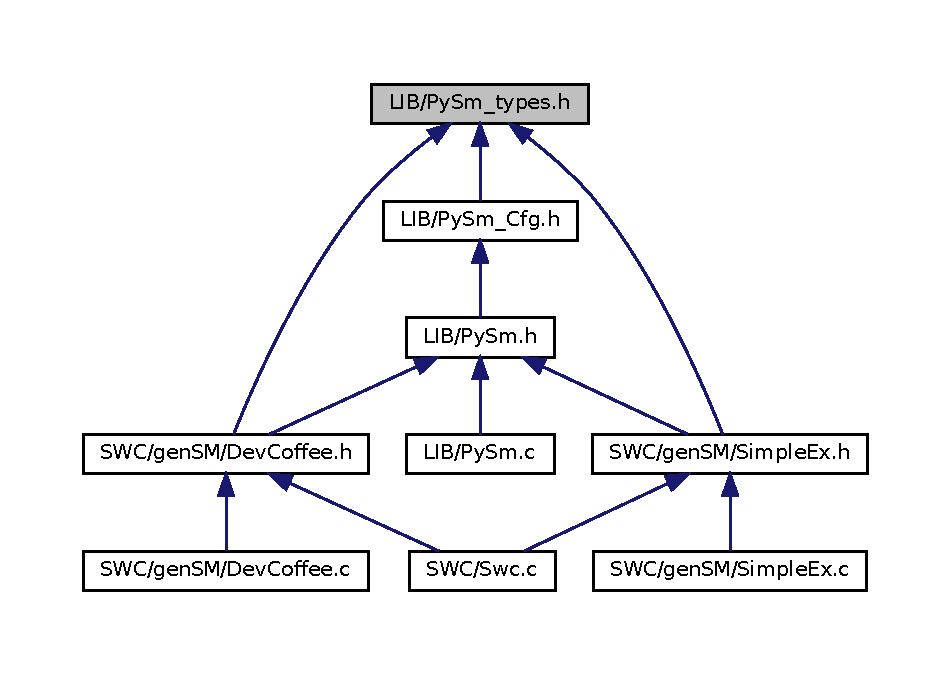
\includegraphics[width=350pt]{PySm__types_8h__dep__incl}
\end{center}
\end{figure}
\subsection*{Macros}
\begin{DoxyCompactItemize}
\item 
\#define \hyperlink{PySm__types_8h_a2d538b28b8c43097dc712c36d8b6557a}{P\+Y\+S\+M\+\_\+\+T\+R\+UE}~1u
\item 
\#define \hyperlink{PySm__types_8h_aa434540dce60703cb46b3270e994d9b5}{P\+Y\+S\+M\+\_\+\+F\+A\+L\+SE}~0u
\item 
\#define \hyperlink{PySm__types_8h_a6791211d32c7477881011bdac53bcf00}{P\+Y\+S\+M\+\_\+\+S\+T\+D\+\_\+\+ON}~1u
\item 
\#define \hyperlink{PySm__types_8h_af27eadac9f8904a12617554c952771b9}{P\+Y\+S\+M\+\_\+\+S\+T\+D\+\_\+\+O\+FF}~0u
\item 
\#define \hyperlink{PySm__types_8h_a2afdb5c4ce56548232a74e689113cb95}{P\+Y\+S\+M\+\_\+\+N\+U\+L\+L\+\_\+\+P\+TR}~(void $\ast$)0
\end{DoxyCompactItemize}
\subsection*{Typedefs}
\begin{DoxyCompactItemize}
\item 
typedef signed char \hyperlink{PySm__types_8h_a76a5be1150c25e18541683a8bd1f0390}{py\+Sm\+\_\+int8}
\item 
typedef short int \hyperlink{PySm__types_8h_a24c3a51a9a0f68a7a60f82e63c90fc8f}{py\+Sm\+\_\+int16}
\item 
typedef int \hyperlink{PySm__types_8h_a760667b6bcc92b6989817a69bc355db3}{py\+Sm\+\_\+int32}
\item 
typedef unsigned char \hyperlink{PySm__types_8h_a1aff40256c00f194609879f8f6f1e1a1}{py\+Sm\+\_\+uint8}
\item 
typedef unsigned short int \hyperlink{PySm__types_8h_a062eb79813ba96aaea55b316b9565111}{py\+Sm\+\_\+uint16}
\item 
typedef unsigned int \hyperlink{PySm__types_8h_a91749d6c36dd467bc6c4253e9a28af40}{py\+Sm\+\_\+uint32}
\item 
typedef unsigned char \hyperlink{PySm__types_8h_a368133d64634d66410f3fe1343de6ba3}{py\+Sm\+\_\+bool}
\end{DoxyCompactItemize}
\subsection*{Variables}
\begin{DoxyCompactItemize}
\item 
\+\_\+\+\_\+extension\+\_\+\+\_\+ typedef long long int \hyperlink{PySm__types_8h_a8d91f4fa5d9f23ef3ab26a93bc984a6a}{py\+Sm\+\_\+int64}
\item 
\+\_\+\+\_\+extension\+\_\+\+\_\+ typedef unsigned long long int \hyperlink{PySm__types_8h_a9c879adcbb717a9d3f5081b5c3a322cc}{py\+Sm\+\_\+uint64}
\end{DoxyCompactItemize}


\subsection{Detailed Description}
File containing basic data types. 

\begin{DoxyAuthor}{Author}
Markus Burger 
\end{DoxyAuthor}
\begin{DoxyDate}{Date}
2017-\/09-\/11 
\end{DoxyDate}


\subsection{Macro Definition Documentation}
\mbox{\Hypertarget{PySm__types_8h_aa434540dce60703cb46b3270e994d9b5}\label{PySm__types_8h_aa434540dce60703cb46b3270e994d9b5}} 
\index{Py\+Sm\+\_\+types.\+h@{Py\+Sm\+\_\+types.\+h}!P\+Y\+S\+M\+\_\+\+F\+A\+L\+SE@{P\+Y\+S\+M\+\_\+\+F\+A\+L\+SE}}
\index{P\+Y\+S\+M\+\_\+\+F\+A\+L\+SE@{P\+Y\+S\+M\+\_\+\+F\+A\+L\+SE}!Py\+Sm\+\_\+types.\+h@{Py\+Sm\+\_\+types.\+h}}
\subsubsection{\texorpdfstring{P\+Y\+S\+M\+\_\+\+F\+A\+L\+SE}{PYSM\_FALSE}}
{\footnotesize\ttfamily \#define P\+Y\+S\+M\+\_\+\+F\+A\+L\+SE~0u}

\mbox{\Hypertarget{PySm__types_8h_a2afdb5c4ce56548232a74e689113cb95}\label{PySm__types_8h_a2afdb5c4ce56548232a74e689113cb95}} 
\index{Py\+Sm\+\_\+types.\+h@{Py\+Sm\+\_\+types.\+h}!P\+Y\+S\+M\+\_\+\+N\+U\+L\+L\+\_\+\+P\+TR@{P\+Y\+S\+M\+\_\+\+N\+U\+L\+L\+\_\+\+P\+TR}}
\index{P\+Y\+S\+M\+\_\+\+N\+U\+L\+L\+\_\+\+P\+TR@{P\+Y\+S\+M\+\_\+\+N\+U\+L\+L\+\_\+\+P\+TR}!Py\+Sm\+\_\+types.\+h@{Py\+Sm\+\_\+types.\+h}}
\subsubsection{\texorpdfstring{P\+Y\+S\+M\+\_\+\+N\+U\+L\+L\+\_\+\+P\+TR}{PYSM\_NULL\_PTR}}
{\footnotesize\ttfamily \#define P\+Y\+S\+M\+\_\+\+N\+U\+L\+L\+\_\+\+P\+TR~(void $\ast$)0}

\mbox{\Hypertarget{PySm__types_8h_af27eadac9f8904a12617554c952771b9}\label{PySm__types_8h_af27eadac9f8904a12617554c952771b9}} 
\index{Py\+Sm\+\_\+types.\+h@{Py\+Sm\+\_\+types.\+h}!P\+Y\+S\+M\+\_\+\+S\+T\+D\+\_\+\+O\+FF@{P\+Y\+S\+M\+\_\+\+S\+T\+D\+\_\+\+O\+FF}}
\index{P\+Y\+S\+M\+\_\+\+S\+T\+D\+\_\+\+O\+FF@{P\+Y\+S\+M\+\_\+\+S\+T\+D\+\_\+\+O\+FF}!Py\+Sm\+\_\+types.\+h@{Py\+Sm\+\_\+types.\+h}}
\subsubsection{\texorpdfstring{P\+Y\+S\+M\+\_\+\+S\+T\+D\+\_\+\+O\+FF}{PYSM\_STD\_OFF}}
{\footnotesize\ttfamily \#define P\+Y\+S\+M\+\_\+\+S\+T\+D\+\_\+\+O\+FF~0u}

\mbox{\Hypertarget{PySm__types_8h_a6791211d32c7477881011bdac53bcf00}\label{PySm__types_8h_a6791211d32c7477881011bdac53bcf00}} 
\index{Py\+Sm\+\_\+types.\+h@{Py\+Sm\+\_\+types.\+h}!P\+Y\+S\+M\+\_\+\+S\+T\+D\+\_\+\+ON@{P\+Y\+S\+M\+\_\+\+S\+T\+D\+\_\+\+ON}}
\index{P\+Y\+S\+M\+\_\+\+S\+T\+D\+\_\+\+ON@{P\+Y\+S\+M\+\_\+\+S\+T\+D\+\_\+\+ON}!Py\+Sm\+\_\+types.\+h@{Py\+Sm\+\_\+types.\+h}}
\subsubsection{\texorpdfstring{P\+Y\+S\+M\+\_\+\+S\+T\+D\+\_\+\+ON}{PYSM\_STD\_ON}}
{\footnotesize\ttfamily \#define P\+Y\+S\+M\+\_\+\+S\+T\+D\+\_\+\+ON~1u}

\mbox{\Hypertarget{PySm__types_8h_a2d538b28b8c43097dc712c36d8b6557a}\label{PySm__types_8h_a2d538b28b8c43097dc712c36d8b6557a}} 
\index{Py\+Sm\+\_\+types.\+h@{Py\+Sm\+\_\+types.\+h}!P\+Y\+S\+M\+\_\+\+T\+R\+UE@{P\+Y\+S\+M\+\_\+\+T\+R\+UE}}
\index{P\+Y\+S\+M\+\_\+\+T\+R\+UE@{P\+Y\+S\+M\+\_\+\+T\+R\+UE}!Py\+Sm\+\_\+types.\+h@{Py\+Sm\+\_\+types.\+h}}
\subsubsection{\texorpdfstring{P\+Y\+S\+M\+\_\+\+T\+R\+UE}{PYSM\_TRUE}}
{\footnotesize\ttfamily \#define P\+Y\+S\+M\+\_\+\+T\+R\+UE~1u}



\subsection{Typedef Documentation}
\mbox{\Hypertarget{PySm__types_8h_a368133d64634d66410f3fe1343de6ba3}\label{PySm__types_8h_a368133d64634d66410f3fe1343de6ba3}} 
\index{Py\+Sm\+\_\+types.\+h@{Py\+Sm\+\_\+types.\+h}!py\+Sm\+\_\+bool@{py\+Sm\+\_\+bool}}
\index{py\+Sm\+\_\+bool@{py\+Sm\+\_\+bool}!Py\+Sm\+\_\+types.\+h@{Py\+Sm\+\_\+types.\+h}}
\subsubsection{\texorpdfstring{py\+Sm\+\_\+bool}{pySm\_bool}}
{\footnotesize\ttfamily typedef unsigned char \hyperlink{PySm__types_8h_a368133d64634d66410f3fe1343de6ba3}{py\+Sm\+\_\+bool}}

\mbox{\Hypertarget{PySm__types_8h_a24c3a51a9a0f68a7a60f82e63c90fc8f}\label{PySm__types_8h_a24c3a51a9a0f68a7a60f82e63c90fc8f}} 
\index{Py\+Sm\+\_\+types.\+h@{Py\+Sm\+\_\+types.\+h}!py\+Sm\+\_\+int16@{py\+Sm\+\_\+int16}}
\index{py\+Sm\+\_\+int16@{py\+Sm\+\_\+int16}!Py\+Sm\+\_\+types.\+h@{Py\+Sm\+\_\+types.\+h}}
\subsubsection{\texorpdfstring{py\+Sm\+\_\+int16}{pySm\_int16}}
{\footnotesize\ttfamily typedef short int \hyperlink{PySm__types_8h_a24c3a51a9a0f68a7a60f82e63c90fc8f}{py\+Sm\+\_\+int16}}

\mbox{\Hypertarget{PySm__types_8h_a760667b6bcc92b6989817a69bc355db3}\label{PySm__types_8h_a760667b6bcc92b6989817a69bc355db3}} 
\index{Py\+Sm\+\_\+types.\+h@{Py\+Sm\+\_\+types.\+h}!py\+Sm\+\_\+int32@{py\+Sm\+\_\+int32}}
\index{py\+Sm\+\_\+int32@{py\+Sm\+\_\+int32}!Py\+Sm\+\_\+types.\+h@{Py\+Sm\+\_\+types.\+h}}
\subsubsection{\texorpdfstring{py\+Sm\+\_\+int32}{pySm\_int32}}
{\footnotesize\ttfamily typedef int \hyperlink{PySm__types_8h_a760667b6bcc92b6989817a69bc355db3}{py\+Sm\+\_\+int32}}

\mbox{\Hypertarget{PySm__types_8h_a76a5be1150c25e18541683a8bd1f0390}\label{PySm__types_8h_a76a5be1150c25e18541683a8bd1f0390}} 
\index{Py\+Sm\+\_\+types.\+h@{Py\+Sm\+\_\+types.\+h}!py\+Sm\+\_\+int8@{py\+Sm\+\_\+int8}}
\index{py\+Sm\+\_\+int8@{py\+Sm\+\_\+int8}!Py\+Sm\+\_\+types.\+h@{Py\+Sm\+\_\+types.\+h}}
\subsubsection{\texorpdfstring{py\+Sm\+\_\+int8}{pySm\_int8}}
{\footnotesize\ttfamily typedef signed char \hyperlink{PySm__types_8h_a76a5be1150c25e18541683a8bd1f0390}{py\+Sm\+\_\+int8}}

\mbox{\Hypertarget{PySm__types_8h_a062eb79813ba96aaea55b316b9565111}\label{PySm__types_8h_a062eb79813ba96aaea55b316b9565111}} 
\index{Py\+Sm\+\_\+types.\+h@{Py\+Sm\+\_\+types.\+h}!py\+Sm\+\_\+uint16@{py\+Sm\+\_\+uint16}}
\index{py\+Sm\+\_\+uint16@{py\+Sm\+\_\+uint16}!Py\+Sm\+\_\+types.\+h@{Py\+Sm\+\_\+types.\+h}}
\subsubsection{\texorpdfstring{py\+Sm\+\_\+uint16}{pySm\_uint16}}
{\footnotesize\ttfamily typedef unsigned short int \hyperlink{PySm__types_8h_a062eb79813ba96aaea55b316b9565111}{py\+Sm\+\_\+uint16}}

\mbox{\Hypertarget{PySm__types_8h_a91749d6c36dd467bc6c4253e9a28af40}\label{PySm__types_8h_a91749d6c36dd467bc6c4253e9a28af40}} 
\index{Py\+Sm\+\_\+types.\+h@{Py\+Sm\+\_\+types.\+h}!py\+Sm\+\_\+uint32@{py\+Sm\+\_\+uint32}}
\index{py\+Sm\+\_\+uint32@{py\+Sm\+\_\+uint32}!Py\+Sm\+\_\+types.\+h@{Py\+Sm\+\_\+types.\+h}}
\subsubsection{\texorpdfstring{py\+Sm\+\_\+uint32}{pySm\_uint32}}
{\footnotesize\ttfamily typedef unsigned int \hyperlink{PySm__types_8h_a91749d6c36dd467bc6c4253e9a28af40}{py\+Sm\+\_\+uint32}}

\mbox{\Hypertarget{PySm__types_8h_a1aff40256c00f194609879f8f6f1e1a1}\label{PySm__types_8h_a1aff40256c00f194609879f8f6f1e1a1}} 
\index{Py\+Sm\+\_\+types.\+h@{Py\+Sm\+\_\+types.\+h}!py\+Sm\+\_\+uint8@{py\+Sm\+\_\+uint8}}
\index{py\+Sm\+\_\+uint8@{py\+Sm\+\_\+uint8}!Py\+Sm\+\_\+types.\+h@{Py\+Sm\+\_\+types.\+h}}
\subsubsection{\texorpdfstring{py\+Sm\+\_\+uint8}{pySm\_uint8}}
{\footnotesize\ttfamily typedef unsigned char \hyperlink{PySm__types_8h_a1aff40256c00f194609879f8f6f1e1a1}{py\+Sm\+\_\+uint8}}



\subsection{Variable Documentation}
\mbox{\Hypertarget{PySm__types_8h_a8d91f4fa5d9f23ef3ab26a93bc984a6a}\label{PySm__types_8h_a8d91f4fa5d9f23ef3ab26a93bc984a6a}} 
\index{Py\+Sm\+\_\+types.\+h@{Py\+Sm\+\_\+types.\+h}!py\+Sm\+\_\+int64@{py\+Sm\+\_\+int64}}
\index{py\+Sm\+\_\+int64@{py\+Sm\+\_\+int64}!Py\+Sm\+\_\+types.\+h@{Py\+Sm\+\_\+types.\+h}}
\subsubsection{\texorpdfstring{py\+Sm\+\_\+int64}{pySm\_int64}}
{\footnotesize\ttfamily \+\_\+\+\_\+extension\+\_\+\+\_\+ typedef long long int py\+Sm\+\_\+int64}

\mbox{\Hypertarget{PySm__types_8h_a9c879adcbb717a9d3f5081b5c3a322cc}\label{PySm__types_8h_a9c879adcbb717a9d3f5081b5c3a322cc}} 
\index{Py\+Sm\+\_\+types.\+h@{Py\+Sm\+\_\+types.\+h}!py\+Sm\+\_\+uint64@{py\+Sm\+\_\+uint64}}
\index{py\+Sm\+\_\+uint64@{py\+Sm\+\_\+uint64}!Py\+Sm\+\_\+types.\+h@{Py\+Sm\+\_\+types.\+h}}
\subsubsection{\texorpdfstring{py\+Sm\+\_\+uint64}{pySm\_uint64}}
{\footnotesize\ttfamily \+\_\+\+\_\+extension\+\_\+\+\_\+ typedef unsigned long long int py\+Sm\+\_\+uint64}


\hypertarget{main_8c}{}\section{main.\+c File Reference}
\label{main_8c}\index{main.\+c@{main.\+c}}


Test main function, calling the test-\/\+S\+WC.  


{\ttfamily \#include \char`\"{}Swc.\+h\char`\"{}}\newline
Include dependency graph for main.\+c\+:\nopagebreak
\begin{figure}[H]
\begin{center}
\leavevmode
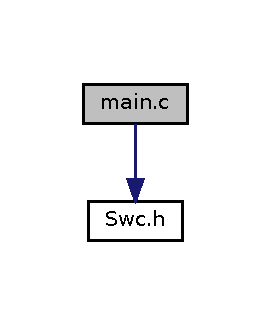
\includegraphics[width=130pt]{main_8c__incl}
\end{center}
\end{figure}
\subsection*{Functions}
\begin{DoxyCompactItemize}
\item 
int \hyperlink{main_8c_a840291bc02cba5474a4cb46a9b9566fe}{main} (void)
\end{DoxyCompactItemize}


\subsection{Detailed Description}
Test main function, calling the test-\/\+S\+WC. 

\begin{DoxyAuthor}{Author}
Markus Burger 
\end{DoxyAuthor}
\begin{DoxyDate}{Date}
2017-\/09-\/11 
\end{DoxyDate}


\subsection{Function Documentation}
\mbox{\Hypertarget{main_8c_a840291bc02cba5474a4cb46a9b9566fe}\label{main_8c_a840291bc02cba5474a4cb46a9b9566fe}} 
\index{main.\+c@{main.\+c}!main@{main}}
\index{main@{main}!main.\+c@{main.\+c}}
\subsubsection{\texorpdfstring{main()}{main()}}
{\footnotesize\ttfamily int main (\begin{DoxyParamCaption}\item[{void}]{ }\end{DoxyParamCaption})}

Here is the call graph for this function\+:
\nopagebreak
\begin{figure}[H]
\begin{center}
\leavevmode
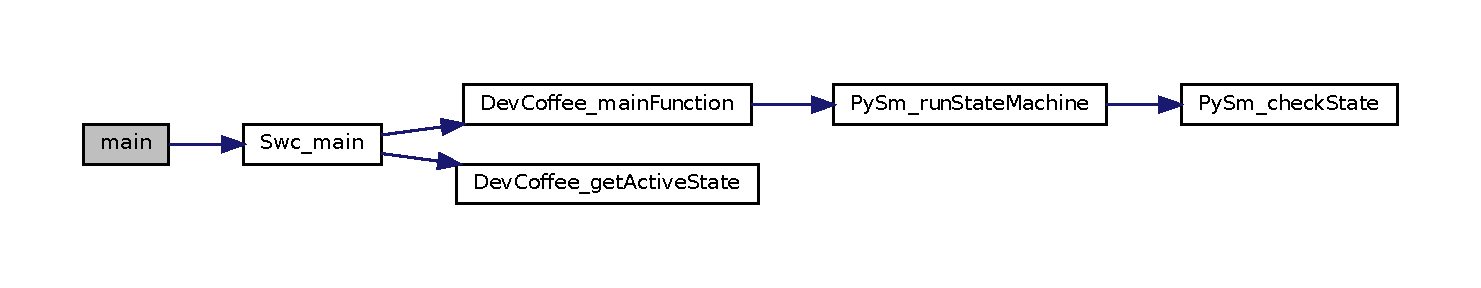
\includegraphics[width=350pt]{main_8c_a840291bc02cba5474a4cb46a9b9566fe_cgraph}
\end{center}
\end{figure}

\hypertarget{DevCoffee_8c}{}\section{S\+W\+C/gen\+S\+M/\+Dev\+Coffee.c File Reference}
\label{DevCoffee_8c}\index{S\+W\+C/gen\+S\+M/\+Dev\+Coffee.\+c@{S\+W\+C/gen\+S\+M/\+Dev\+Coffee.\+c}}


Header for generated state machine dev\+Coffee Generated 2017-\/09-\/27 19\+:41\+:10 by Py\+SM -\/ The python state machine generator.  


{\ttfamily \#include \char`\"{}Dev\+Coffee.\+h\char`\"{}}\newline
Include dependency graph for Dev\+Coffee.\+c\+:
\nopagebreak
\begin{figure}[H]
\begin{center}
\leavevmode
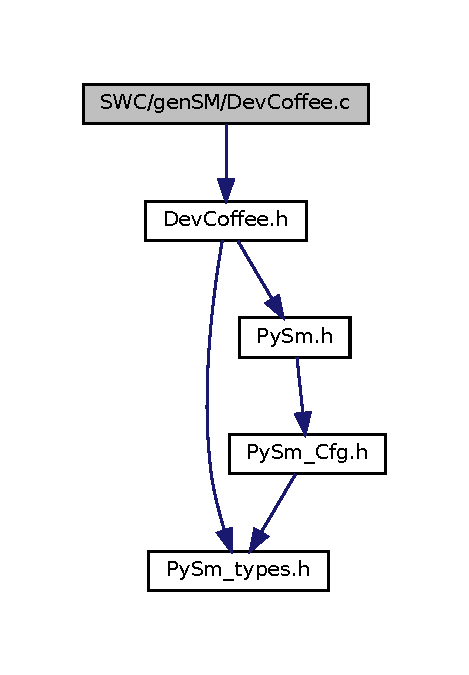
\includegraphics[width=225pt]{DevCoffee_8c__incl}
\end{center}
\end{figure}
\subsection*{Functions}
\begin{DoxyCompactItemize}
\item 
static void \hyperlink{DevCoffee_8c_a6693558189e3c9ae878baaf3cb639be0}{dev\+Coffee\+\_\+\+S\+F\+\_\+\+B\+R\+E\+A\+K\+F\+A\+S\+T\+\_\+entry} (void)
\item 
static void \hyperlink{DevCoffee_8c_a3ddae66ae84b979e65af9364a4272510}{dev\+Coffee\+\_\+\+S\+F\+\_\+\+B\+R\+E\+A\+K\+F\+A\+ST} (void)
\item 
static void \hyperlink{DevCoffee_8c_aa1b8f1a36fc117510933afe38bb7a571}{dev\+Coffee\+\_\+\+S\+F\+\_\+\+B\+R\+E\+A\+K\+F\+A\+S\+T\+\_\+exit} (void)
\item 
static void \hyperlink{DevCoffee_8c_af9813f5643c8eeb32f4b8b494b91a8ce}{dev\+Coffee\+\_\+\+S\+F\+\_\+\+I\+N\+\_\+\+O\+F\+F\+I\+C\+E\+\_\+entry} (void)
\item 
static void \hyperlink{DevCoffee_8c_ac5294be70d2633f6384d2145fcdcf624}{dev\+Coffee\+\_\+\+S\+F\+\_\+\+I\+N\+\_\+\+O\+F\+F\+I\+CE} (void)
\item 
static void \hyperlink{DevCoffee_8c_a5436f937c7804fc4aa212e3d5906f8c1}{dev\+Coffee\+\_\+\+S\+F\+\_\+\+G\+E\+T\+\_\+\+C\+O\+F\+F\+E\+E\+\_\+entry} (void)
\item 
static void \hyperlink{DevCoffee_8c_aa5a0b123092c0da9413a823e7bf42ce5}{dev\+Coffee\+\_\+\+S\+F\+\_\+\+R\+E\+L\+A\+X\+\_\+\+A\+N\+D\+\_\+\+S\+L\+E\+E\+P\+\_\+entry} (void)
\item 
static void \hyperlink{DevCoffee_8c_a6c84040c8d0ceab6709eb6a1070de5d8}{dev\+Coffee\+\_\+\+S\+F\+\_\+\+R\+E\+L\+A\+X\+\_\+\+A\+N\+D\+\_\+\+S\+L\+E\+EP} (void)
\item 
static void \hyperlink{DevCoffee_8c_ae6dd5236124c24bed053c8d5a8d6167e}{dev\+Coffee\+\_\+\+S\+F\+\_\+\+D\+E\+V\+E\+L\+O\+P\+E\+R\+\_\+\+I\+S\+\_\+\+I\+L\+L\+\_\+entry} (void)
\item 
static void \hyperlink{DevCoffee_8c_aff0df3606e88e11de53219b469982f6f}{dev\+Coffee\+\_\+\+S\+F\+\_\+\+D\+E\+V\+E\+L\+O\+P\+E\+R\+\_\+\+I\+S\+\_\+\+I\+LL} (void)
\item 
static void \hyperlink{DevCoffee_8c_a4b7d09fe3f64bd7fabbe109802f5b2c1}{dev\+Coffee\+\_\+variable\+Reset\+Function} (void)
\item 
static \hyperlink{PySm__types_8h_a368133d64634d66410f3fe1343de6ba3}{py\+Sm\+\_\+bool} \hyperlink{DevCoffee_8c_aa6a3e42e5b9b76beec93c6614b02b72d}{dev\+Coffee\+\_\+\+T\+T\+F\+\_\+\+I\+N\+\_\+\+O\+F\+F\+I\+C\+E\+\_\+to\+\_\+\+I\+N\+\_\+\+O\+F\+F\+I\+CE} (void)
\item 
static \hyperlink{PySm__types_8h_a368133d64634d66410f3fe1343de6ba3}{py\+Sm\+\_\+bool} \hyperlink{DevCoffee_8c_a6f3bae6b3d8787b7fe5cb08c8fb73c7d}{dev\+Coffee\+\_\+\+T\+T\+F\+\_\+\+B\+R\+E\+A\+K\+F\+A\+S\+T\+\_\+to\+\_\+\+I\+N\+\_\+\+O\+F\+F\+I\+CE} (void)
\item 
static \hyperlink{PySm__types_8h_a368133d64634d66410f3fe1343de6ba3}{py\+Sm\+\_\+bool} \hyperlink{DevCoffee_8c_a036cb7388037dd6b276fcf043e34b29a}{dev\+Coffee\+\_\+\+T\+T\+F\+\_\+\+I\+N\+\_\+\+O\+F\+F\+I\+C\+E\+\_\+to\+\_\+\+G\+E\+T\+\_\+\+C\+O\+F\+F\+EE} (void)
\item 
static \hyperlink{PySm__types_8h_a368133d64634d66410f3fe1343de6ba3}{py\+Sm\+\_\+bool} \hyperlink{DevCoffee_8c_a4f153d1f06088c508c71a18eb4c5e1b8}{dev\+Coffee\+\_\+\+T\+T\+F\+\_\+\+I\+N\+\_\+\+O\+F\+F\+I\+C\+E\+\_\+to\+\_\+\+R\+E\+L\+A\+X\+\_\+\+A\+N\+D\+\_\+\+S\+L\+E\+EP} (void)
\item 
static \hyperlink{PySm__types_8h_a368133d64634d66410f3fe1343de6ba3}{py\+Sm\+\_\+bool} \hyperlink{DevCoffee_8c_afbc64528ca9f2e5f773722497e92f572}{dev\+Coffee\+\_\+\+T\+T\+F\+\_\+\+R\+E\+L\+A\+X\+\_\+\+A\+N\+D\+\_\+\+S\+L\+E\+E\+P\+\_\+to\+\_\+\+B\+R\+E\+A\+K\+F\+A\+S\+T\+\_\+1} (void)
\item 
static \hyperlink{PySm__types_8h_a368133d64634d66410f3fe1343de6ba3}{py\+Sm\+\_\+bool} \hyperlink{DevCoffee_8c_a1ad7ad09d448d354c98b8398b6ed5d63}{dev\+Coffee\+\_\+\+T\+T\+F\+\_\+\+B\+R\+E\+A\+K\+F\+A\+S\+T\+\_\+to\+\_\+\+D\+E\+V\+E\+L\+O\+P\+E\+R\+\_\+\+I\+S\+\_\+\+I\+LL} (void)
\item 
static \hyperlink{PySm__types_8h_a368133d64634d66410f3fe1343de6ba3}{py\+Sm\+\_\+bool} \hyperlink{DevCoffee_8c_a9a1ddcec23b201e76a0d885b9bd0dc95}{dev\+Coffee\+\_\+\+T\+T\+F\+\_\+\+D\+E\+V\+E\+L\+O\+P\+E\+R\+\_\+\+I\+S\+\_\+\+I\+L\+L\+\_\+to\+\_\+\+B\+R\+E\+A\+K\+F\+A\+ST} (void)
\item 
static \hyperlink{PySm__types_8h_a368133d64634d66410f3fe1343de6ba3}{py\+Sm\+\_\+bool} \hyperlink{DevCoffee_8c_ad46de6ebf46162d3daa8a4c408cd9699}{dev\+Coffee\+\_\+\+T\+T\+F\+\_\+\+R\+E\+L\+A\+X\+\_\+\+A\+N\+D\+\_\+\+S\+L\+E\+E\+P\+\_\+to\+\_\+\+B\+R\+E\+A\+K\+F\+A\+S\+T\+\_\+2} (void)
\item 
static void \hyperlink{DevCoffee_8c_a55240048578d7980fd95adb42179f9d1}{dev\+Coffee\+\_\+\+T\+A\+F\+\_\+\+I\+N\+\_\+\+O\+F\+F\+I\+C\+E\+\_\+to\+\_\+\+I\+N\+\_\+\+O\+F\+F\+I\+CE} (void)
\item 
static void \hyperlink{DevCoffee_8c_a457d603d8ec08f2c1d7401f55f22405a}{dev\+Coffee\+\_\+\+T\+A\+F\+\_\+\+G\+E\+T\+\_\+\+C\+O\+F\+F\+E\+E\+\_\+to\+\_\+\+I\+N\+\_\+\+O\+F\+F\+I\+CE} (void)
\item 
static void \hyperlink{DevCoffee_8c_aa169c26bfeaa1dcc2546b4aaaa53d1cf}{dev\+Coffee\+\_\+\+T\+A\+F\+\_\+\+I\+N\+\_\+\+O\+F\+F\+I\+C\+E\+\_\+to\+\_\+\+R\+E\+L\+A\+X\+\_\+\+A\+N\+D\+\_\+\+S\+L\+E\+EP} (void)
\item 
static void \hyperlink{DevCoffee_8c_a09cbb4f4282a9264c4226d75290f9bad}{dev\+Coffee\+\_\+\+T\+A\+F\+\_\+\+R\+E\+L\+A\+X\+\_\+\+A\+N\+D\+\_\+\+S\+L\+E\+E\+P\+\_\+to\+\_\+\+B\+R\+E\+A\+K\+F\+A\+ST} (void)
\item 
\hyperlink{PySm_8h_a1bd760b7300136bf7e0bd7b9e3a126ff}{py\+Sm\+\_\+return\+Type} \hyperlink{DevCoffee_8c_a9957d470d0f0c12d7268e1f7027afe98}{Dev\+Coffee\+\_\+main\+Function} (\hyperlink{structdevCoffee__inputSignalsType}{dev\+Coffee\+\_\+input\+Signals\+Type} $\ast$swc\+\_\+input\+Signals, \hyperlink{structdevCoffee__outputSignalsType}{dev\+Coffee\+\_\+output\+Signals\+Type} $\ast$swc\+\_\+output\+Signals)
\begin{DoxyCompactList}\small\item\em Main function of the state machine dev\+Coffee. \end{DoxyCompactList}\item 
void \hyperlink{DevCoffee_8c_a4a1714b386a18a4d8f8b8cdc7639cf8e}{Dev\+Coffee\+\_\+get\+Active\+State} (\hyperlink{DevCoffee_8h_a5590d50a72c7655d28dc92f0531c26dc}{dev\+Coffee\+\_\+active\+State\+Type} $\ast$swc\+\_\+active\+State)
\begin{DoxyCompactList}\small\item\em Main function of the state machine dev\+Coffee. \end{DoxyCompactList}\end{DoxyCompactItemize}
\subsection*{Variables}
\begin{DoxyCompactItemize}
\item 
static const \hyperlink{structpySm__stateType}{py\+Sm\+\_\+state\+Type} \hyperlink{DevCoffee_8c_af69f95cd452fb1a8107fb0c24b55dbfe}{dev\+Coffee\+\_\+state\+\_\+\+B\+R\+E\+A\+K\+F\+A\+ST}
\item 
static const \hyperlink{structpySm__stateType}{py\+Sm\+\_\+state\+Type} \hyperlink{DevCoffee_8c_a813864d9823f9e8546377aa1d31276b9}{dev\+Coffee\+\_\+state\+\_\+\+I\+N\+\_\+\+O\+F\+F\+I\+CE}
\item 
static const \hyperlink{structpySm__stateType}{py\+Sm\+\_\+state\+Type} \hyperlink{DevCoffee_8c_a84297d04424307cf775ef35349dbad69}{dev\+Coffee\+\_\+state\+\_\+\+G\+E\+T\+\_\+\+C\+O\+F\+F\+EE}
\item 
static const \hyperlink{structpySm__stateType}{py\+Sm\+\_\+state\+Type} \hyperlink{DevCoffee_8c_ad3eac650dbd4217e848edf18a6f82ba2}{dev\+Coffee\+\_\+state\+\_\+\+R\+E\+L\+A\+X\+\_\+\+A\+N\+D\+\_\+\+S\+L\+E\+EP}
\item 
static const \hyperlink{structpySm__stateType}{py\+Sm\+\_\+state\+Type} \hyperlink{DevCoffee_8c_a6eefe16888efe003681428c1f8a9e7be}{dev\+Coffee\+\_\+state\+\_\+\+D\+E\+V\+E\+L\+O\+P\+E\+R\+\_\+\+I\+S\+\_\+\+I\+LL}
\item 
static const \hyperlink{structpySm__stateType}{py\+Sm\+\_\+state\+Type} $\ast$ \hyperlink{DevCoffee_8c_aa5aa3d69dad032a8efd8877b1ef27bff}{dev\+Coffee\+\_\+states\+\_\+pa} \mbox{[}5\mbox{]}
\item 
static \hyperlink{structpySm__stateTransitionType}{py\+Sm\+\_\+state\+Transition\+Type} \hyperlink{DevCoffee_8c_a9cbcc3e5213cb70fc7fad36c62e67d24}{dev\+Coffee\+\_\+transitions\+\_\+sa} \mbox{[}9\mbox{]}
\item 
\hyperlink{structpySm__stateMachineType}{py\+Sm\+\_\+state\+Machine\+Type} \hyperlink{DevCoffee_8c_a5de158962931debff85f11d6098497f7}{dev\+Coffee\+\_\+state\+Machine\+\_\+s}
\item 
static \hyperlink{structdevCoffee__inputSignalsType}{dev\+Coffee\+\_\+input\+Signals\+Type} $\ast$ \hyperlink{DevCoffee_8c_a21c7dd8abf1338d313341dc86910f83b}{dev\+Coffee\+\_\+input\+Signals}
\item 
static \hyperlink{structdevCoffee__outputSignalsType}{dev\+Coffee\+\_\+output\+Signals\+Type} $\ast$ \hyperlink{DevCoffee_8c_a1e6bf7869d3bb76b2e4e41615d49120a}{dev\+Coffee\+\_\+output\+Signals}
\item 
static \hyperlink{DevCoffee_8h_a5590d50a72c7655d28dc92f0531c26dc}{dev\+Coffee\+\_\+active\+State\+Type} \hyperlink{DevCoffee_8c_ae0a60a7566081901de7dd4fb2da7b2b2}{dev\+Coffee\+\_\+active\+State} = \hyperlink{DevCoffee_8h_a5590d50a72c7655d28dc92f0531c26dca5c79ab73bc31ae6cd575cb28ce078adc}{dev\+Coffee\+\_\+\+U\+N\+I\+N\+I\+T\+A\+L\+I\+Z\+E\+D\+\_\+\+S\+T\+A\+T\+E\+\_\+\+M\+A\+C\+H\+I\+NE}
\item 
\hyperlink{PySm__types_8h_a1aff40256c00f194609879f8f6f1e1a1}{py\+Sm\+\_\+uint8} \hyperlink{DevCoffee_8c_a635b0516c139160b6a4a171d92a92b9c}{coffeein\+\_\+level\+\_\+ui8} = 0u
\item 
\hyperlink{PySm__types_8h_a1aff40256c00f194609879f8f6f1e1a1}{py\+Sm\+\_\+uint8} \hyperlink{DevCoffee_8c_ad80ad5d06b5b105acfc60db98ee885ed}{productivity\+\_\+ui8} = 0u
\item 
\hyperlink{PySm__types_8h_a1aff40256c00f194609879f8f6f1e1a1}{py\+Sm\+\_\+uint8} \hyperlink{DevCoffee_8c_a399d06b6bbd6c404b9281de41cbd79e0}{current\+\_\+hour\+\_\+ui8} = 0u
\end{DoxyCompactItemize}


\subsection{Detailed Description}
Header for generated state machine dev\+Coffee Generated 2017-\/09-\/27 19\+:41\+:10 by Py\+SM -\/ The python state machine generator. 

\begin{DoxyAuthor}{Author}
Markus 
\end{DoxyAuthor}
\begin{DoxyDate}{Date}
2017-\/09-\/27 
\end{DoxyDate}


\subsection{Function Documentation}
\mbox{\Hypertarget{DevCoffee_8c_a4a1714b386a18a4d8f8b8cdc7639cf8e}\label{DevCoffee_8c_a4a1714b386a18a4d8f8b8cdc7639cf8e}} 
\index{Dev\+Coffee.\+c@{Dev\+Coffee.\+c}!Dev\+Coffee\+\_\+get\+Active\+State@{Dev\+Coffee\+\_\+get\+Active\+State}}
\index{Dev\+Coffee\+\_\+get\+Active\+State@{Dev\+Coffee\+\_\+get\+Active\+State}!Dev\+Coffee.\+c@{Dev\+Coffee.\+c}}
\subsubsection{\texorpdfstring{Dev\+Coffee\+\_\+get\+Active\+State()}{DevCoffee\_getActiveState()}}
{\footnotesize\ttfamily void Dev\+Coffee\+\_\+get\+Active\+State (\begin{DoxyParamCaption}\item[{\hyperlink{DevCoffee_8h_a5590d50a72c7655d28dc92f0531c26dc}{dev\+Coffee\+\_\+active\+State\+Type} $\ast$}]{swc\+\_\+active\+State }\end{DoxyParamCaption})}



Main function of the state machine dev\+Coffee. 

\mbox{\Hypertarget{DevCoffee_8c_a9957d470d0f0c12d7268e1f7027afe98}\label{DevCoffee_8c_a9957d470d0f0c12d7268e1f7027afe98}} 
\index{Dev\+Coffee.\+c@{Dev\+Coffee.\+c}!Dev\+Coffee\+\_\+main\+Function@{Dev\+Coffee\+\_\+main\+Function}}
\index{Dev\+Coffee\+\_\+main\+Function@{Dev\+Coffee\+\_\+main\+Function}!Dev\+Coffee.\+c@{Dev\+Coffee.\+c}}
\subsubsection{\texorpdfstring{Dev\+Coffee\+\_\+main\+Function()}{DevCoffee\_mainFunction()}}
{\footnotesize\ttfamily \hyperlink{PySm_8h_a1bd760b7300136bf7e0bd7b9e3a126ff}{py\+Sm\+\_\+return\+Type} Dev\+Coffee\+\_\+main\+Function (\begin{DoxyParamCaption}\item[{\hyperlink{structdevCoffee__inputSignalsType}{dev\+Coffee\+\_\+input\+Signals\+Type} $\ast$}]{swc\+\_\+input\+Signals,  }\item[{\hyperlink{structdevCoffee__outputSignalsType}{dev\+Coffee\+\_\+output\+Signals\+Type} $\ast$}]{swc\+\_\+output\+Signals }\end{DoxyParamCaption})}



Main function of the state machine dev\+Coffee. 

Here is the call graph for this function\+:\nopagebreak
\begin{figure}[H]
\begin{center}
\leavevmode
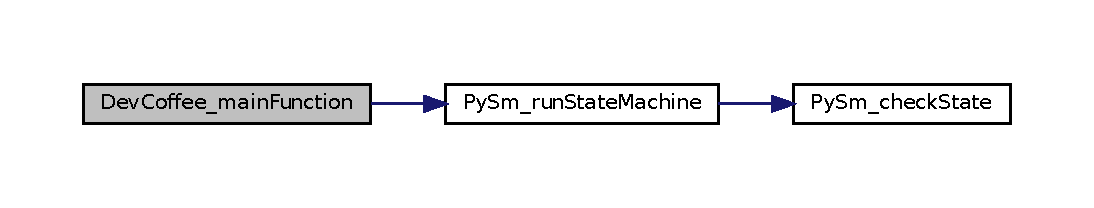
\includegraphics[width=350pt]{DevCoffee_8c_a9957d470d0f0c12d7268e1f7027afe98_cgraph}
\end{center}
\end{figure}
\mbox{\Hypertarget{DevCoffee_8c_a3ddae66ae84b979e65af9364a4272510}\label{DevCoffee_8c_a3ddae66ae84b979e65af9364a4272510}} 
\index{Dev\+Coffee.\+c@{Dev\+Coffee.\+c}!dev\+Coffee\+\_\+\+S\+F\+\_\+\+B\+R\+E\+A\+K\+F\+A\+ST@{dev\+Coffee\+\_\+\+S\+F\+\_\+\+B\+R\+E\+A\+K\+F\+A\+ST}}
\index{dev\+Coffee\+\_\+\+S\+F\+\_\+\+B\+R\+E\+A\+K\+F\+A\+ST@{dev\+Coffee\+\_\+\+S\+F\+\_\+\+B\+R\+E\+A\+K\+F\+A\+ST}!Dev\+Coffee.\+c@{Dev\+Coffee.\+c}}
\subsubsection{\texorpdfstring{dev\+Coffee\+\_\+\+S\+F\+\_\+\+B\+R\+E\+A\+K\+F\+A\+S\+T()}{devCoffee\_SF\_BREAKFAST()}}
{\footnotesize\ttfamily static void dev\+Coffee\+\_\+\+S\+F\+\_\+\+B\+R\+E\+A\+K\+F\+A\+ST (\begin{DoxyParamCaption}\item[{void}]{ }\end{DoxyParamCaption})\hspace{0.3cm}{\ttfamily [static]}}

\mbox{\Hypertarget{DevCoffee_8c_a6693558189e3c9ae878baaf3cb639be0}\label{DevCoffee_8c_a6693558189e3c9ae878baaf3cb639be0}} 
\index{Dev\+Coffee.\+c@{Dev\+Coffee.\+c}!dev\+Coffee\+\_\+\+S\+F\+\_\+\+B\+R\+E\+A\+K\+F\+A\+S\+T\+\_\+entry@{dev\+Coffee\+\_\+\+S\+F\+\_\+\+B\+R\+E\+A\+K\+F\+A\+S\+T\+\_\+entry}}
\index{dev\+Coffee\+\_\+\+S\+F\+\_\+\+B\+R\+E\+A\+K\+F\+A\+S\+T\+\_\+entry@{dev\+Coffee\+\_\+\+S\+F\+\_\+\+B\+R\+E\+A\+K\+F\+A\+S\+T\+\_\+entry}!Dev\+Coffee.\+c@{Dev\+Coffee.\+c}}
\subsubsection{\texorpdfstring{dev\+Coffee\+\_\+\+S\+F\+\_\+\+B\+R\+E\+A\+K\+F\+A\+S\+T\+\_\+entry()}{devCoffee\_SF\_BREAKFAST\_entry()}}
{\footnotesize\ttfamily static void dev\+Coffee\+\_\+\+S\+F\+\_\+\+B\+R\+E\+A\+K\+F\+A\+S\+T\+\_\+entry (\begin{DoxyParamCaption}\item[{void}]{ }\end{DoxyParamCaption})\hspace{0.3cm}{\ttfamily [static]}}

\mbox{\Hypertarget{DevCoffee_8c_aa1b8f1a36fc117510933afe38bb7a571}\label{DevCoffee_8c_aa1b8f1a36fc117510933afe38bb7a571}} 
\index{Dev\+Coffee.\+c@{Dev\+Coffee.\+c}!dev\+Coffee\+\_\+\+S\+F\+\_\+\+B\+R\+E\+A\+K\+F\+A\+S\+T\+\_\+exit@{dev\+Coffee\+\_\+\+S\+F\+\_\+\+B\+R\+E\+A\+K\+F\+A\+S\+T\+\_\+exit}}
\index{dev\+Coffee\+\_\+\+S\+F\+\_\+\+B\+R\+E\+A\+K\+F\+A\+S\+T\+\_\+exit@{dev\+Coffee\+\_\+\+S\+F\+\_\+\+B\+R\+E\+A\+K\+F\+A\+S\+T\+\_\+exit}!Dev\+Coffee.\+c@{Dev\+Coffee.\+c}}
\subsubsection{\texorpdfstring{dev\+Coffee\+\_\+\+S\+F\+\_\+\+B\+R\+E\+A\+K\+F\+A\+S\+T\+\_\+exit()}{devCoffee\_SF\_BREAKFAST\_exit()}}
{\footnotesize\ttfamily static void dev\+Coffee\+\_\+\+S\+F\+\_\+\+B\+R\+E\+A\+K\+F\+A\+S\+T\+\_\+exit (\begin{DoxyParamCaption}\item[{void}]{ }\end{DoxyParamCaption})\hspace{0.3cm}{\ttfamily [static]}}

\mbox{\Hypertarget{DevCoffee_8c_aff0df3606e88e11de53219b469982f6f}\label{DevCoffee_8c_aff0df3606e88e11de53219b469982f6f}} 
\index{Dev\+Coffee.\+c@{Dev\+Coffee.\+c}!dev\+Coffee\+\_\+\+S\+F\+\_\+\+D\+E\+V\+E\+L\+O\+P\+E\+R\+\_\+\+I\+S\+\_\+\+I\+LL@{dev\+Coffee\+\_\+\+S\+F\+\_\+\+D\+E\+V\+E\+L\+O\+P\+E\+R\+\_\+\+I\+S\+\_\+\+I\+LL}}
\index{dev\+Coffee\+\_\+\+S\+F\+\_\+\+D\+E\+V\+E\+L\+O\+P\+E\+R\+\_\+\+I\+S\+\_\+\+I\+LL@{dev\+Coffee\+\_\+\+S\+F\+\_\+\+D\+E\+V\+E\+L\+O\+P\+E\+R\+\_\+\+I\+S\+\_\+\+I\+LL}!Dev\+Coffee.\+c@{Dev\+Coffee.\+c}}
\subsubsection{\texorpdfstring{dev\+Coffee\+\_\+\+S\+F\+\_\+\+D\+E\+V\+E\+L\+O\+P\+E\+R\+\_\+\+I\+S\+\_\+\+I\+L\+L()}{devCoffee\_SF\_DEVELOPER\_IS\_ILL()}}
{\footnotesize\ttfamily static void dev\+Coffee\+\_\+\+S\+F\+\_\+\+D\+E\+V\+E\+L\+O\+P\+E\+R\+\_\+\+I\+S\+\_\+\+I\+LL (\begin{DoxyParamCaption}\item[{void}]{ }\end{DoxyParamCaption})\hspace{0.3cm}{\ttfamily [static]}}

\mbox{\Hypertarget{DevCoffee_8c_ae6dd5236124c24bed053c8d5a8d6167e}\label{DevCoffee_8c_ae6dd5236124c24bed053c8d5a8d6167e}} 
\index{Dev\+Coffee.\+c@{Dev\+Coffee.\+c}!dev\+Coffee\+\_\+\+S\+F\+\_\+\+D\+E\+V\+E\+L\+O\+P\+E\+R\+\_\+\+I\+S\+\_\+\+I\+L\+L\+\_\+entry@{dev\+Coffee\+\_\+\+S\+F\+\_\+\+D\+E\+V\+E\+L\+O\+P\+E\+R\+\_\+\+I\+S\+\_\+\+I\+L\+L\+\_\+entry}}
\index{dev\+Coffee\+\_\+\+S\+F\+\_\+\+D\+E\+V\+E\+L\+O\+P\+E\+R\+\_\+\+I\+S\+\_\+\+I\+L\+L\+\_\+entry@{dev\+Coffee\+\_\+\+S\+F\+\_\+\+D\+E\+V\+E\+L\+O\+P\+E\+R\+\_\+\+I\+S\+\_\+\+I\+L\+L\+\_\+entry}!Dev\+Coffee.\+c@{Dev\+Coffee.\+c}}
\subsubsection{\texorpdfstring{dev\+Coffee\+\_\+\+S\+F\+\_\+\+D\+E\+V\+E\+L\+O\+P\+E\+R\+\_\+\+I\+S\+\_\+\+I\+L\+L\+\_\+entry()}{devCoffee\_SF\_DEVELOPER\_IS\_ILL\_entry()}}
{\footnotesize\ttfamily static void dev\+Coffee\+\_\+\+S\+F\+\_\+\+D\+E\+V\+E\+L\+O\+P\+E\+R\+\_\+\+I\+S\+\_\+\+I\+L\+L\+\_\+entry (\begin{DoxyParamCaption}\item[{void}]{ }\end{DoxyParamCaption})\hspace{0.3cm}{\ttfamily [static]}}

\mbox{\Hypertarget{DevCoffee_8c_a5436f937c7804fc4aa212e3d5906f8c1}\label{DevCoffee_8c_a5436f937c7804fc4aa212e3d5906f8c1}} 
\index{Dev\+Coffee.\+c@{Dev\+Coffee.\+c}!dev\+Coffee\+\_\+\+S\+F\+\_\+\+G\+E\+T\+\_\+\+C\+O\+F\+F\+E\+E\+\_\+entry@{dev\+Coffee\+\_\+\+S\+F\+\_\+\+G\+E\+T\+\_\+\+C\+O\+F\+F\+E\+E\+\_\+entry}}
\index{dev\+Coffee\+\_\+\+S\+F\+\_\+\+G\+E\+T\+\_\+\+C\+O\+F\+F\+E\+E\+\_\+entry@{dev\+Coffee\+\_\+\+S\+F\+\_\+\+G\+E\+T\+\_\+\+C\+O\+F\+F\+E\+E\+\_\+entry}!Dev\+Coffee.\+c@{Dev\+Coffee.\+c}}
\subsubsection{\texorpdfstring{dev\+Coffee\+\_\+\+S\+F\+\_\+\+G\+E\+T\+\_\+\+C\+O\+F\+F\+E\+E\+\_\+entry()}{devCoffee\_SF\_GET\_COFFEE\_entry()}}
{\footnotesize\ttfamily static void dev\+Coffee\+\_\+\+S\+F\+\_\+\+G\+E\+T\+\_\+\+C\+O\+F\+F\+E\+E\+\_\+entry (\begin{DoxyParamCaption}\item[{void}]{ }\end{DoxyParamCaption})\hspace{0.3cm}{\ttfamily [static]}}

\mbox{\Hypertarget{DevCoffee_8c_ac5294be70d2633f6384d2145fcdcf624}\label{DevCoffee_8c_ac5294be70d2633f6384d2145fcdcf624}} 
\index{Dev\+Coffee.\+c@{Dev\+Coffee.\+c}!dev\+Coffee\+\_\+\+S\+F\+\_\+\+I\+N\+\_\+\+O\+F\+F\+I\+CE@{dev\+Coffee\+\_\+\+S\+F\+\_\+\+I\+N\+\_\+\+O\+F\+F\+I\+CE}}
\index{dev\+Coffee\+\_\+\+S\+F\+\_\+\+I\+N\+\_\+\+O\+F\+F\+I\+CE@{dev\+Coffee\+\_\+\+S\+F\+\_\+\+I\+N\+\_\+\+O\+F\+F\+I\+CE}!Dev\+Coffee.\+c@{Dev\+Coffee.\+c}}
\subsubsection{\texorpdfstring{dev\+Coffee\+\_\+\+S\+F\+\_\+\+I\+N\+\_\+\+O\+F\+F\+I\+C\+E()}{devCoffee\_SF\_IN\_OFFICE()}}
{\footnotesize\ttfamily static void dev\+Coffee\+\_\+\+S\+F\+\_\+\+I\+N\+\_\+\+O\+F\+F\+I\+CE (\begin{DoxyParamCaption}\item[{void}]{ }\end{DoxyParamCaption})\hspace{0.3cm}{\ttfamily [static]}}

\mbox{\Hypertarget{DevCoffee_8c_af9813f5643c8eeb32f4b8b494b91a8ce}\label{DevCoffee_8c_af9813f5643c8eeb32f4b8b494b91a8ce}} 
\index{Dev\+Coffee.\+c@{Dev\+Coffee.\+c}!dev\+Coffee\+\_\+\+S\+F\+\_\+\+I\+N\+\_\+\+O\+F\+F\+I\+C\+E\+\_\+entry@{dev\+Coffee\+\_\+\+S\+F\+\_\+\+I\+N\+\_\+\+O\+F\+F\+I\+C\+E\+\_\+entry}}
\index{dev\+Coffee\+\_\+\+S\+F\+\_\+\+I\+N\+\_\+\+O\+F\+F\+I\+C\+E\+\_\+entry@{dev\+Coffee\+\_\+\+S\+F\+\_\+\+I\+N\+\_\+\+O\+F\+F\+I\+C\+E\+\_\+entry}!Dev\+Coffee.\+c@{Dev\+Coffee.\+c}}
\subsubsection{\texorpdfstring{dev\+Coffee\+\_\+\+S\+F\+\_\+\+I\+N\+\_\+\+O\+F\+F\+I\+C\+E\+\_\+entry()}{devCoffee\_SF\_IN\_OFFICE\_entry()}}
{\footnotesize\ttfamily static void dev\+Coffee\+\_\+\+S\+F\+\_\+\+I\+N\+\_\+\+O\+F\+F\+I\+C\+E\+\_\+entry (\begin{DoxyParamCaption}\item[{void}]{ }\end{DoxyParamCaption})\hspace{0.3cm}{\ttfamily [static]}}

\mbox{\Hypertarget{DevCoffee_8c_a6c84040c8d0ceab6709eb6a1070de5d8}\label{DevCoffee_8c_a6c84040c8d0ceab6709eb6a1070de5d8}} 
\index{Dev\+Coffee.\+c@{Dev\+Coffee.\+c}!dev\+Coffee\+\_\+\+S\+F\+\_\+\+R\+E\+L\+A\+X\+\_\+\+A\+N\+D\+\_\+\+S\+L\+E\+EP@{dev\+Coffee\+\_\+\+S\+F\+\_\+\+R\+E\+L\+A\+X\+\_\+\+A\+N\+D\+\_\+\+S\+L\+E\+EP}}
\index{dev\+Coffee\+\_\+\+S\+F\+\_\+\+R\+E\+L\+A\+X\+\_\+\+A\+N\+D\+\_\+\+S\+L\+E\+EP@{dev\+Coffee\+\_\+\+S\+F\+\_\+\+R\+E\+L\+A\+X\+\_\+\+A\+N\+D\+\_\+\+S\+L\+E\+EP}!Dev\+Coffee.\+c@{Dev\+Coffee.\+c}}
\subsubsection{\texorpdfstring{dev\+Coffee\+\_\+\+S\+F\+\_\+\+R\+E\+L\+A\+X\+\_\+\+A\+N\+D\+\_\+\+S\+L\+E\+E\+P()}{devCoffee\_SF\_RELAX\_AND\_SLEEP()}}
{\footnotesize\ttfamily static void dev\+Coffee\+\_\+\+S\+F\+\_\+\+R\+E\+L\+A\+X\+\_\+\+A\+N\+D\+\_\+\+S\+L\+E\+EP (\begin{DoxyParamCaption}\item[{void}]{ }\end{DoxyParamCaption})\hspace{0.3cm}{\ttfamily [static]}}

\mbox{\Hypertarget{DevCoffee_8c_aa5a0b123092c0da9413a823e7bf42ce5}\label{DevCoffee_8c_aa5a0b123092c0da9413a823e7bf42ce5}} 
\index{Dev\+Coffee.\+c@{Dev\+Coffee.\+c}!dev\+Coffee\+\_\+\+S\+F\+\_\+\+R\+E\+L\+A\+X\+\_\+\+A\+N\+D\+\_\+\+S\+L\+E\+E\+P\+\_\+entry@{dev\+Coffee\+\_\+\+S\+F\+\_\+\+R\+E\+L\+A\+X\+\_\+\+A\+N\+D\+\_\+\+S\+L\+E\+E\+P\+\_\+entry}}
\index{dev\+Coffee\+\_\+\+S\+F\+\_\+\+R\+E\+L\+A\+X\+\_\+\+A\+N\+D\+\_\+\+S\+L\+E\+E\+P\+\_\+entry@{dev\+Coffee\+\_\+\+S\+F\+\_\+\+R\+E\+L\+A\+X\+\_\+\+A\+N\+D\+\_\+\+S\+L\+E\+E\+P\+\_\+entry}!Dev\+Coffee.\+c@{Dev\+Coffee.\+c}}
\subsubsection{\texorpdfstring{dev\+Coffee\+\_\+\+S\+F\+\_\+\+R\+E\+L\+A\+X\+\_\+\+A\+N\+D\+\_\+\+S\+L\+E\+E\+P\+\_\+entry()}{devCoffee\_SF\_RELAX\_AND\_SLEEP\_entry()}}
{\footnotesize\ttfamily static void dev\+Coffee\+\_\+\+S\+F\+\_\+\+R\+E\+L\+A\+X\+\_\+\+A\+N\+D\+\_\+\+S\+L\+E\+E\+P\+\_\+entry (\begin{DoxyParamCaption}\item[{void}]{ }\end{DoxyParamCaption})\hspace{0.3cm}{\ttfamily [static]}}

\mbox{\Hypertarget{DevCoffee_8c_a457d603d8ec08f2c1d7401f55f22405a}\label{DevCoffee_8c_a457d603d8ec08f2c1d7401f55f22405a}} 
\index{Dev\+Coffee.\+c@{Dev\+Coffee.\+c}!dev\+Coffee\+\_\+\+T\+A\+F\+\_\+\+G\+E\+T\+\_\+\+C\+O\+F\+F\+E\+E\+\_\+to\+\_\+\+I\+N\+\_\+\+O\+F\+F\+I\+CE@{dev\+Coffee\+\_\+\+T\+A\+F\+\_\+\+G\+E\+T\+\_\+\+C\+O\+F\+F\+E\+E\+\_\+to\+\_\+\+I\+N\+\_\+\+O\+F\+F\+I\+CE}}
\index{dev\+Coffee\+\_\+\+T\+A\+F\+\_\+\+G\+E\+T\+\_\+\+C\+O\+F\+F\+E\+E\+\_\+to\+\_\+\+I\+N\+\_\+\+O\+F\+F\+I\+CE@{dev\+Coffee\+\_\+\+T\+A\+F\+\_\+\+G\+E\+T\+\_\+\+C\+O\+F\+F\+E\+E\+\_\+to\+\_\+\+I\+N\+\_\+\+O\+F\+F\+I\+CE}!Dev\+Coffee.\+c@{Dev\+Coffee.\+c}}
\subsubsection{\texorpdfstring{dev\+Coffee\+\_\+\+T\+A\+F\+\_\+\+G\+E\+T\+\_\+\+C\+O\+F\+F\+E\+E\+\_\+to\+\_\+\+I\+N\+\_\+\+O\+F\+F\+I\+C\+E()}{devCoffee\_TAF\_GET\_COFFEE\_to\_IN\_OFFICE()}}
{\footnotesize\ttfamily static void dev\+Coffee\+\_\+\+T\+A\+F\+\_\+\+G\+E\+T\+\_\+\+C\+O\+F\+F\+E\+E\+\_\+to\+\_\+\+I\+N\+\_\+\+O\+F\+F\+I\+CE (\begin{DoxyParamCaption}\item[{void}]{ }\end{DoxyParamCaption})\hspace{0.3cm}{\ttfamily [static]}}

\mbox{\Hypertarget{DevCoffee_8c_a55240048578d7980fd95adb42179f9d1}\label{DevCoffee_8c_a55240048578d7980fd95adb42179f9d1}} 
\index{Dev\+Coffee.\+c@{Dev\+Coffee.\+c}!dev\+Coffee\+\_\+\+T\+A\+F\+\_\+\+I\+N\+\_\+\+O\+F\+F\+I\+C\+E\+\_\+to\+\_\+\+I\+N\+\_\+\+O\+F\+F\+I\+CE@{dev\+Coffee\+\_\+\+T\+A\+F\+\_\+\+I\+N\+\_\+\+O\+F\+F\+I\+C\+E\+\_\+to\+\_\+\+I\+N\+\_\+\+O\+F\+F\+I\+CE}}
\index{dev\+Coffee\+\_\+\+T\+A\+F\+\_\+\+I\+N\+\_\+\+O\+F\+F\+I\+C\+E\+\_\+to\+\_\+\+I\+N\+\_\+\+O\+F\+F\+I\+CE@{dev\+Coffee\+\_\+\+T\+A\+F\+\_\+\+I\+N\+\_\+\+O\+F\+F\+I\+C\+E\+\_\+to\+\_\+\+I\+N\+\_\+\+O\+F\+F\+I\+CE}!Dev\+Coffee.\+c@{Dev\+Coffee.\+c}}
\subsubsection{\texorpdfstring{dev\+Coffee\+\_\+\+T\+A\+F\+\_\+\+I\+N\+\_\+\+O\+F\+F\+I\+C\+E\+\_\+to\+\_\+\+I\+N\+\_\+\+O\+F\+F\+I\+C\+E()}{devCoffee\_TAF\_IN\_OFFICE\_to\_IN\_OFFICE()}}
{\footnotesize\ttfamily static void dev\+Coffee\+\_\+\+T\+A\+F\+\_\+\+I\+N\+\_\+\+O\+F\+F\+I\+C\+E\+\_\+to\+\_\+\+I\+N\+\_\+\+O\+F\+F\+I\+CE (\begin{DoxyParamCaption}\item[{void}]{ }\end{DoxyParamCaption})\hspace{0.3cm}{\ttfamily [static]}}

\mbox{\Hypertarget{DevCoffee_8c_aa169c26bfeaa1dcc2546b4aaaa53d1cf}\label{DevCoffee_8c_aa169c26bfeaa1dcc2546b4aaaa53d1cf}} 
\index{Dev\+Coffee.\+c@{Dev\+Coffee.\+c}!dev\+Coffee\+\_\+\+T\+A\+F\+\_\+\+I\+N\+\_\+\+O\+F\+F\+I\+C\+E\+\_\+to\+\_\+\+R\+E\+L\+A\+X\+\_\+\+A\+N\+D\+\_\+\+S\+L\+E\+EP@{dev\+Coffee\+\_\+\+T\+A\+F\+\_\+\+I\+N\+\_\+\+O\+F\+F\+I\+C\+E\+\_\+to\+\_\+\+R\+E\+L\+A\+X\+\_\+\+A\+N\+D\+\_\+\+S\+L\+E\+EP}}
\index{dev\+Coffee\+\_\+\+T\+A\+F\+\_\+\+I\+N\+\_\+\+O\+F\+F\+I\+C\+E\+\_\+to\+\_\+\+R\+E\+L\+A\+X\+\_\+\+A\+N\+D\+\_\+\+S\+L\+E\+EP@{dev\+Coffee\+\_\+\+T\+A\+F\+\_\+\+I\+N\+\_\+\+O\+F\+F\+I\+C\+E\+\_\+to\+\_\+\+R\+E\+L\+A\+X\+\_\+\+A\+N\+D\+\_\+\+S\+L\+E\+EP}!Dev\+Coffee.\+c@{Dev\+Coffee.\+c}}
\subsubsection{\texorpdfstring{dev\+Coffee\+\_\+\+T\+A\+F\+\_\+\+I\+N\+\_\+\+O\+F\+F\+I\+C\+E\+\_\+to\+\_\+\+R\+E\+L\+A\+X\+\_\+\+A\+N\+D\+\_\+\+S\+L\+E\+E\+P()}{devCoffee\_TAF\_IN\_OFFICE\_to\_RELAX\_AND\_SLEEP()}}
{\footnotesize\ttfamily static void dev\+Coffee\+\_\+\+T\+A\+F\+\_\+\+I\+N\+\_\+\+O\+F\+F\+I\+C\+E\+\_\+to\+\_\+\+R\+E\+L\+A\+X\+\_\+\+A\+N\+D\+\_\+\+S\+L\+E\+EP (\begin{DoxyParamCaption}\item[{void}]{ }\end{DoxyParamCaption})\hspace{0.3cm}{\ttfamily [static]}}

\mbox{\Hypertarget{DevCoffee_8c_a09cbb4f4282a9264c4226d75290f9bad}\label{DevCoffee_8c_a09cbb4f4282a9264c4226d75290f9bad}} 
\index{Dev\+Coffee.\+c@{Dev\+Coffee.\+c}!dev\+Coffee\+\_\+\+T\+A\+F\+\_\+\+R\+E\+L\+A\+X\+\_\+\+A\+N\+D\+\_\+\+S\+L\+E\+E\+P\+\_\+to\+\_\+\+B\+R\+E\+A\+K\+F\+A\+ST@{dev\+Coffee\+\_\+\+T\+A\+F\+\_\+\+R\+E\+L\+A\+X\+\_\+\+A\+N\+D\+\_\+\+S\+L\+E\+E\+P\+\_\+to\+\_\+\+B\+R\+E\+A\+K\+F\+A\+ST}}
\index{dev\+Coffee\+\_\+\+T\+A\+F\+\_\+\+R\+E\+L\+A\+X\+\_\+\+A\+N\+D\+\_\+\+S\+L\+E\+E\+P\+\_\+to\+\_\+\+B\+R\+E\+A\+K\+F\+A\+ST@{dev\+Coffee\+\_\+\+T\+A\+F\+\_\+\+R\+E\+L\+A\+X\+\_\+\+A\+N\+D\+\_\+\+S\+L\+E\+E\+P\+\_\+to\+\_\+\+B\+R\+E\+A\+K\+F\+A\+ST}!Dev\+Coffee.\+c@{Dev\+Coffee.\+c}}
\subsubsection{\texorpdfstring{dev\+Coffee\+\_\+\+T\+A\+F\+\_\+\+R\+E\+L\+A\+X\+\_\+\+A\+N\+D\+\_\+\+S\+L\+E\+E\+P\+\_\+to\+\_\+\+B\+R\+E\+A\+K\+F\+A\+S\+T()}{devCoffee\_TAF\_RELAX\_AND\_SLEEP\_to\_BREAKFAST()}}
{\footnotesize\ttfamily static void dev\+Coffee\+\_\+\+T\+A\+F\+\_\+\+R\+E\+L\+A\+X\+\_\+\+A\+N\+D\+\_\+\+S\+L\+E\+E\+P\+\_\+to\+\_\+\+B\+R\+E\+A\+K\+F\+A\+ST (\begin{DoxyParamCaption}\item[{void}]{ }\end{DoxyParamCaption})\hspace{0.3cm}{\ttfamily [static]}}

\mbox{\Hypertarget{DevCoffee_8c_a1ad7ad09d448d354c98b8398b6ed5d63}\label{DevCoffee_8c_a1ad7ad09d448d354c98b8398b6ed5d63}} 
\index{Dev\+Coffee.\+c@{Dev\+Coffee.\+c}!dev\+Coffee\+\_\+\+T\+T\+F\+\_\+\+B\+R\+E\+A\+K\+F\+A\+S\+T\+\_\+to\+\_\+\+D\+E\+V\+E\+L\+O\+P\+E\+R\+\_\+\+I\+S\+\_\+\+I\+LL@{dev\+Coffee\+\_\+\+T\+T\+F\+\_\+\+B\+R\+E\+A\+K\+F\+A\+S\+T\+\_\+to\+\_\+\+D\+E\+V\+E\+L\+O\+P\+E\+R\+\_\+\+I\+S\+\_\+\+I\+LL}}
\index{dev\+Coffee\+\_\+\+T\+T\+F\+\_\+\+B\+R\+E\+A\+K\+F\+A\+S\+T\+\_\+to\+\_\+\+D\+E\+V\+E\+L\+O\+P\+E\+R\+\_\+\+I\+S\+\_\+\+I\+LL@{dev\+Coffee\+\_\+\+T\+T\+F\+\_\+\+B\+R\+E\+A\+K\+F\+A\+S\+T\+\_\+to\+\_\+\+D\+E\+V\+E\+L\+O\+P\+E\+R\+\_\+\+I\+S\+\_\+\+I\+LL}!Dev\+Coffee.\+c@{Dev\+Coffee.\+c}}
\subsubsection{\texorpdfstring{dev\+Coffee\+\_\+\+T\+T\+F\+\_\+\+B\+R\+E\+A\+K\+F\+A\+S\+T\+\_\+to\+\_\+\+D\+E\+V\+E\+L\+O\+P\+E\+R\+\_\+\+I\+S\+\_\+\+I\+L\+L()}{devCoffee\_TTF\_BREAKFAST\_to\_DEVELOPER\_IS\_ILL()}}
{\footnotesize\ttfamily static \hyperlink{PySm__types_8h_a368133d64634d66410f3fe1343de6ba3}{py\+Sm\+\_\+bool} dev\+Coffee\+\_\+\+T\+T\+F\+\_\+\+B\+R\+E\+A\+K\+F\+A\+S\+T\+\_\+to\+\_\+\+D\+E\+V\+E\+L\+O\+P\+E\+R\+\_\+\+I\+S\+\_\+\+I\+LL (\begin{DoxyParamCaption}\item[{void}]{ }\end{DoxyParamCaption})\hspace{0.3cm}{\ttfamily [static]}}

\mbox{\Hypertarget{DevCoffee_8c_a6f3bae6b3d8787b7fe5cb08c8fb73c7d}\label{DevCoffee_8c_a6f3bae6b3d8787b7fe5cb08c8fb73c7d}} 
\index{Dev\+Coffee.\+c@{Dev\+Coffee.\+c}!dev\+Coffee\+\_\+\+T\+T\+F\+\_\+\+B\+R\+E\+A\+K\+F\+A\+S\+T\+\_\+to\+\_\+\+I\+N\+\_\+\+O\+F\+F\+I\+CE@{dev\+Coffee\+\_\+\+T\+T\+F\+\_\+\+B\+R\+E\+A\+K\+F\+A\+S\+T\+\_\+to\+\_\+\+I\+N\+\_\+\+O\+F\+F\+I\+CE}}
\index{dev\+Coffee\+\_\+\+T\+T\+F\+\_\+\+B\+R\+E\+A\+K\+F\+A\+S\+T\+\_\+to\+\_\+\+I\+N\+\_\+\+O\+F\+F\+I\+CE@{dev\+Coffee\+\_\+\+T\+T\+F\+\_\+\+B\+R\+E\+A\+K\+F\+A\+S\+T\+\_\+to\+\_\+\+I\+N\+\_\+\+O\+F\+F\+I\+CE}!Dev\+Coffee.\+c@{Dev\+Coffee.\+c}}
\subsubsection{\texorpdfstring{dev\+Coffee\+\_\+\+T\+T\+F\+\_\+\+B\+R\+E\+A\+K\+F\+A\+S\+T\+\_\+to\+\_\+\+I\+N\+\_\+\+O\+F\+F\+I\+C\+E()}{devCoffee\_TTF\_BREAKFAST\_to\_IN\_OFFICE()}}
{\footnotesize\ttfamily static \hyperlink{PySm__types_8h_a368133d64634d66410f3fe1343de6ba3}{py\+Sm\+\_\+bool} dev\+Coffee\+\_\+\+T\+T\+F\+\_\+\+B\+R\+E\+A\+K\+F\+A\+S\+T\+\_\+to\+\_\+\+I\+N\+\_\+\+O\+F\+F\+I\+CE (\begin{DoxyParamCaption}\item[{void}]{ }\end{DoxyParamCaption})\hspace{0.3cm}{\ttfamily [static]}}

\mbox{\Hypertarget{DevCoffee_8c_a9a1ddcec23b201e76a0d885b9bd0dc95}\label{DevCoffee_8c_a9a1ddcec23b201e76a0d885b9bd0dc95}} 
\index{Dev\+Coffee.\+c@{Dev\+Coffee.\+c}!dev\+Coffee\+\_\+\+T\+T\+F\+\_\+\+D\+E\+V\+E\+L\+O\+P\+E\+R\+\_\+\+I\+S\+\_\+\+I\+L\+L\+\_\+to\+\_\+\+B\+R\+E\+A\+K\+F\+A\+ST@{dev\+Coffee\+\_\+\+T\+T\+F\+\_\+\+D\+E\+V\+E\+L\+O\+P\+E\+R\+\_\+\+I\+S\+\_\+\+I\+L\+L\+\_\+to\+\_\+\+B\+R\+E\+A\+K\+F\+A\+ST}}
\index{dev\+Coffee\+\_\+\+T\+T\+F\+\_\+\+D\+E\+V\+E\+L\+O\+P\+E\+R\+\_\+\+I\+S\+\_\+\+I\+L\+L\+\_\+to\+\_\+\+B\+R\+E\+A\+K\+F\+A\+ST@{dev\+Coffee\+\_\+\+T\+T\+F\+\_\+\+D\+E\+V\+E\+L\+O\+P\+E\+R\+\_\+\+I\+S\+\_\+\+I\+L\+L\+\_\+to\+\_\+\+B\+R\+E\+A\+K\+F\+A\+ST}!Dev\+Coffee.\+c@{Dev\+Coffee.\+c}}
\subsubsection{\texorpdfstring{dev\+Coffee\+\_\+\+T\+T\+F\+\_\+\+D\+E\+V\+E\+L\+O\+P\+E\+R\+\_\+\+I\+S\+\_\+\+I\+L\+L\+\_\+to\+\_\+\+B\+R\+E\+A\+K\+F\+A\+S\+T()}{devCoffee\_TTF\_DEVELOPER\_IS\_ILL\_to\_BREAKFAST()}}
{\footnotesize\ttfamily static \hyperlink{PySm__types_8h_a368133d64634d66410f3fe1343de6ba3}{py\+Sm\+\_\+bool} dev\+Coffee\+\_\+\+T\+T\+F\+\_\+\+D\+E\+V\+E\+L\+O\+P\+E\+R\+\_\+\+I\+S\+\_\+\+I\+L\+L\+\_\+to\+\_\+\+B\+R\+E\+A\+K\+F\+A\+ST (\begin{DoxyParamCaption}\item[{void}]{ }\end{DoxyParamCaption})\hspace{0.3cm}{\ttfamily [static]}}

\mbox{\Hypertarget{DevCoffee_8c_a036cb7388037dd6b276fcf043e34b29a}\label{DevCoffee_8c_a036cb7388037dd6b276fcf043e34b29a}} 
\index{Dev\+Coffee.\+c@{Dev\+Coffee.\+c}!dev\+Coffee\+\_\+\+T\+T\+F\+\_\+\+I\+N\+\_\+\+O\+F\+F\+I\+C\+E\+\_\+to\+\_\+\+G\+E\+T\+\_\+\+C\+O\+F\+F\+EE@{dev\+Coffee\+\_\+\+T\+T\+F\+\_\+\+I\+N\+\_\+\+O\+F\+F\+I\+C\+E\+\_\+to\+\_\+\+G\+E\+T\+\_\+\+C\+O\+F\+F\+EE}}
\index{dev\+Coffee\+\_\+\+T\+T\+F\+\_\+\+I\+N\+\_\+\+O\+F\+F\+I\+C\+E\+\_\+to\+\_\+\+G\+E\+T\+\_\+\+C\+O\+F\+F\+EE@{dev\+Coffee\+\_\+\+T\+T\+F\+\_\+\+I\+N\+\_\+\+O\+F\+F\+I\+C\+E\+\_\+to\+\_\+\+G\+E\+T\+\_\+\+C\+O\+F\+F\+EE}!Dev\+Coffee.\+c@{Dev\+Coffee.\+c}}
\subsubsection{\texorpdfstring{dev\+Coffee\+\_\+\+T\+T\+F\+\_\+\+I\+N\+\_\+\+O\+F\+F\+I\+C\+E\+\_\+to\+\_\+\+G\+E\+T\+\_\+\+C\+O\+F\+F\+E\+E()}{devCoffee\_TTF\_IN\_OFFICE\_to\_GET\_COFFEE()}}
{\footnotesize\ttfamily static \hyperlink{PySm__types_8h_a368133d64634d66410f3fe1343de6ba3}{py\+Sm\+\_\+bool} dev\+Coffee\+\_\+\+T\+T\+F\+\_\+\+I\+N\+\_\+\+O\+F\+F\+I\+C\+E\+\_\+to\+\_\+\+G\+E\+T\+\_\+\+C\+O\+F\+F\+EE (\begin{DoxyParamCaption}\item[{void}]{ }\end{DoxyParamCaption})\hspace{0.3cm}{\ttfamily [static]}}

\mbox{\Hypertarget{DevCoffee_8c_aa6a3e42e5b9b76beec93c6614b02b72d}\label{DevCoffee_8c_aa6a3e42e5b9b76beec93c6614b02b72d}} 
\index{Dev\+Coffee.\+c@{Dev\+Coffee.\+c}!dev\+Coffee\+\_\+\+T\+T\+F\+\_\+\+I\+N\+\_\+\+O\+F\+F\+I\+C\+E\+\_\+to\+\_\+\+I\+N\+\_\+\+O\+F\+F\+I\+CE@{dev\+Coffee\+\_\+\+T\+T\+F\+\_\+\+I\+N\+\_\+\+O\+F\+F\+I\+C\+E\+\_\+to\+\_\+\+I\+N\+\_\+\+O\+F\+F\+I\+CE}}
\index{dev\+Coffee\+\_\+\+T\+T\+F\+\_\+\+I\+N\+\_\+\+O\+F\+F\+I\+C\+E\+\_\+to\+\_\+\+I\+N\+\_\+\+O\+F\+F\+I\+CE@{dev\+Coffee\+\_\+\+T\+T\+F\+\_\+\+I\+N\+\_\+\+O\+F\+F\+I\+C\+E\+\_\+to\+\_\+\+I\+N\+\_\+\+O\+F\+F\+I\+CE}!Dev\+Coffee.\+c@{Dev\+Coffee.\+c}}
\subsubsection{\texorpdfstring{dev\+Coffee\+\_\+\+T\+T\+F\+\_\+\+I\+N\+\_\+\+O\+F\+F\+I\+C\+E\+\_\+to\+\_\+\+I\+N\+\_\+\+O\+F\+F\+I\+C\+E()}{devCoffee\_TTF\_IN\_OFFICE\_to\_IN\_OFFICE()}}
{\footnotesize\ttfamily static \hyperlink{PySm__types_8h_a368133d64634d66410f3fe1343de6ba3}{py\+Sm\+\_\+bool} dev\+Coffee\+\_\+\+T\+T\+F\+\_\+\+I\+N\+\_\+\+O\+F\+F\+I\+C\+E\+\_\+to\+\_\+\+I\+N\+\_\+\+O\+F\+F\+I\+CE (\begin{DoxyParamCaption}\item[{void}]{ }\end{DoxyParamCaption})\hspace{0.3cm}{\ttfamily [static]}}

\mbox{\Hypertarget{DevCoffee_8c_a4f153d1f06088c508c71a18eb4c5e1b8}\label{DevCoffee_8c_a4f153d1f06088c508c71a18eb4c5e1b8}} 
\index{Dev\+Coffee.\+c@{Dev\+Coffee.\+c}!dev\+Coffee\+\_\+\+T\+T\+F\+\_\+\+I\+N\+\_\+\+O\+F\+F\+I\+C\+E\+\_\+to\+\_\+\+R\+E\+L\+A\+X\+\_\+\+A\+N\+D\+\_\+\+S\+L\+E\+EP@{dev\+Coffee\+\_\+\+T\+T\+F\+\_\+\+I\+N\+\_\+\+O\+F\+F\+I\+C\+E\+\_\+to\+\_\+\+R\+E\+L\+A\+X\+\_\+\+A\+N\+D\+\_\+\+S\+L\+E\+EP}}
\index{dev\+Coffee\+\_\+\+T\+T\+F\+\_\+\+I\+N\+\_\+\+O\+F\+F\+I\+C\+E\+\_\+to\+\_\+\+R\+E\+L\+A\+X\+\_\+\+A\+N\+D\+\_\+\+S\+L\+E\+EP@{dev\+Coffee\+\_\+\+T\+T\+F\+\_\+\+I\+N\+\_\+\+O\+F\+F\+I\+C\+E\+\_\+to\+\_\+\+R\+E\+L\+A\+X\+\_\+\+A\+N\+D\+\_\+\+S\+L\+E\+EP}!Dev\+Coffee.\+c@{Dev\+Coffee.\+c}}
\subsubsection{\texorpdfstring{dev\+Coffee\+\_\+\+T\+T\+F\+\_\+\+I\+N\+\_\+\+O\+F\+F\+I\+C\+E\+\_\+to\+\_\+\+R\+E\+L\+A\+X\+\_\+\+A\+N\+D\+\_\+\+S\+L\+E\+E\+P()}{devCoffee\_TTF\_IN\_OFFICE\_to\_RELAX\_AND\_SLEEP()}}
{\footnotesize\ttfamily static \hyperlink{PySm__types_8h_a368133d64634d66410f3fe1343de6ba3}{py\+Sm\+\_\+bool} dev\+Coffee\+\_\+\+T\+T\+F\+\_\+\+I\+N\+\_\+\+O\+F\+F\+I\+C\+E\+\_\+to\+\_\+\+R\+E\+L\+A\+X\+\_\+\+A\+N\+D\+\_\+\+S\+L\+E\+EP (\begin{DoxyParamCaption}\item[{void}]{ }\end{DoxyParamCaption})\hspace{0.3cm}{\ttfamily [static]}}

\mbox{\Hypertarget{DevCoffee_8c_afbc64528ca9f2e5f773722497e92f572}\label{DevCoffee_8c_afbc64528ca9f2e5f773722497e92f572}} 
\index{Dev\+Coffee.\+c@{Dev\+Coffee.\+c}!dev\+Coffee\+\_\+\+T\+T\+F\+\_\+\+R\+E\+L\+A\+X\+\_\+\+A\+N\+D\+\_\+\+S\+L\+E\+E\+P\+\_\+to\+\_\+\+B\+R\+E\+A\+K\+F\+A\+S\+T\+\_\+1@{dev\+Coffee\+\_\+\+T\+T\+F\+\_\+\+R\+E\+L\+A\+X\+\_\+\+A\+N\+D\+\_\+\+S\+L\+E\+E\+P\+\_\+to\+\_\+\+B\+R\+E\+A\+K\+F\+A\+S\+T\+\_\+1}}
\index{dev\+Coffee\+\_\+\+T\+T\+F\+\_\+\+R\+E\+L\+A\+X\+\_\+\+A\+N\+D\+\_\+\+S\+L\+E\+E\+P\+\_\+to\+\_\+\+B\+R\+E\+A\+K\+F\+A\+S\+T\+\_\+1@{dev\+Coffee\+\_\+\+T\+T\+F\+\_\+\+R\+E\+L\+A\+X\+\_\+\+A\+N\+D\+\_\+\+S\+L\+E\+E\+P\+\_\+to\+\_\+\+B\+R\+E\+A\+K\+F\+A\+S\+T\+\_\+1}!Dev\+Coffee.\+c@{Dev\+Coffee.\+c}}
\subsubsection{\texorpdfstring{dev\+Coffee\+\_\+\+T\+T\+F\+\_\+\+R\+E\+L\+A\+X\+\_\+\+A\+N\+D\+\_\+\+S\+L\+E\+E\+P\+\_\+to\+\_\+\+B\+R\+E\+A\+K\+F\+A\+S\+T\+\_\+1()}{devCoffee\_TTF\_RELAX\_AND\_SLEEP\_to\_BREAKFAST\_1()}}
{\footnotesize\ttfamily static \hyperlink{PySm__types_8h_a368133d64634d66410f3fe1343de6ba3}{py\+Sm\+\_\+bool} dev\+Coffee\+\_\+\+T\+T\+F\+\_\+\+R\+E\+L\+A\+X\+\_\+\+A\+N\+D\+\_\+\+S\+L\+E\+E\+P\+\_\+to\+\_\+\+B\+R\+E\+A\+K\+F\+A\+S\+T\+\_\+1 (\begin{DoxyParamCaption}\item[{void}]{ }\end{DoxyParamCaption})\hspace{0.3cm}{\ttfamily [static]}}

\mbox{\Hypertarget{DevCoffee_8c_ad46de6ebf46162d3daa8a4c408cd9699}\label{DevCoffee_8c_ad46de6ebf46162d3daa8a4c408cd9699}} 
\index{Dev\+Coffee.\+c@{Dev\+Coffee.\+c}!dev\+Coffee\+\_\+\+T\+T\+F\+\_\+\+R\+E\+L\+A\+X\+\_\+\+A\+N\+D\+\_\+\+S\+L\+E\+E\+P\+\_\+to\+\_\+\+B\+R\+E\+A\+K\+F\+A\+S\+T\+\_\+2@{dev\+Coffee\+\_\+\+T\+T\+F\+\_\+\+R\+E\+L\+A\+X\+\_\+\+A\+N\+D\+\_\+\+S\+L\+E\+E\+P\+\_\+to\+\_\+\+B\+R\+E\+A\+K\+F\+A\+S\+T\+\_\+2}}
\index{dev\+Coffee\+\_\+\+T\+T\+F\+\_\+\+R\+E\+L\+A\+X\+\_\+\+A\+N\+D\+\_\+\+S\+L\+E\+E\+P\+\_\+to\+\_\+\+B\+R\+E\+A\+K\+F\+A\+S\+T\+\_\+2@{dev\+Coffee\+\_\+\+T\+T\+F\+\_\+\+R\+E\+L\+A\+X\+\_\+\+A\+N\+D\+\_\+\+S\+L\+E\+E\+P\+\_\+to\+\_\+\+B\+R\+E\+A\+K\+F\+A\+S\+T\+\_\+2}!Dev\+Coffee.\+c@{Dev\+Coffee.\+c}}
\subsubsection{\texorpdfstring{dev\+Coffee\+\_\+\+T\+T\+F\+\_\+\+R\+E\+L\+A\+X\+\_\+\+A\+N\+D\+\_\+\+S\+L\+E\+E\+P\+\_\+to\+\_\+\+B\+R\+E\+A\+K\+F\+A\+S\+T\+\_\+2()}{devCoffee\_TTF\_RELAX\_AND\_SLEEP\_to\_BREAKFAST\_2()}}
{\footnotesize\ttfamily static \hyperlink{PySm__types_8h_a368133d64634d66410f3fe1343de6ba3}{py\+Sm\+\_\+bool} dev\+Coffee\+\_\+\+T\+T\+F\+\_\+\+R\+E\+L\+A\+X\+\_\+\+A\+N\+D\+\_\+\+S\+L\+E\+E\+P\+\_\+to\+\_\+\+B\+R\+E\+A\+K\+F\+A\+S\+T\+\_\+2 (\begin{DoxyParamCaption}\item[{void}]{ }\end{DoxyParamCaption})\hspace{0.3cm}{\ttfamily [static]}}

\mbox{\Hypertarget{DevCoffee_8c_a4b7d09fe3f64bd7fabbe109802f5b2c1}\label{DevCoffee_8c_a4b7d09fe3f64bd7fabbe109802f5b2c1}} 
\index{Dev\+Coffee.\+c@{Dev\+Coffee.\+c}!dev\+Coffee\+\_\+variable\+Reset\+Function@{dev\+Coffee\+\_\+variable\+Reset\+Function}}
\index{dev\+Coffee\+\_\+variable\+Reset\+Function@{dev\+Coffee\+\_\+variable\+Reset\+Function}!Dev\+Coffee.\+c@{Dev\+Coffee.\+c}}
\subsubsection{\texorpdfstring{dev\+Coffee\+\_\+variable\+Reset\+Function()}{devCoffee\_variableResetFunction()}}
{\footnotesize\ttfamily static void dev\+Coffee\+\_\+variable\+Reset\+Function (\begin{DoxyParamCaption}\item[{void}]{ }\end{DoxyParamCaption})\hspace{0.3cm}{\ttfamily [static]}}



\subsection{Variable Documentation}
\mbox{\Hypertarget{DevCoffee_8c_a635b0516c139160b6a4a171d92a92b9c}\label{DevCoffee_8c_a635b0516c139160b6a4a171d92a92b9c}} 
\index{Dev\+Coffee.\+c@{Dev\+Coffee.\+c}!coffeein\+\_\+level\+\_\+ui8@{coffeein\+\_\+level\+\_\+ui8}}
\index{coffeein\+\_\+level\+\_\+ui8@{coffeein\+\_\+level\+\_\+ui8}!Dev\+Coffee.\+c@{Dev\+Coffee.\+c}}
\subsubsection{\texorpdfstring{coffeein\+\_\+level\+\_\+ui8}{coffeein\_level\_ui8}}
{\footnotesize\ttfamily \hyperlink{PySm__types_8h_a1aff40256c00f194609879f8f6f1e1a1}{py\+Sm\+\_\+uint8} coffeein\+\_\+level\+\_\+ui8 = 0u}

\mbox{\Hypertarget{DevCoffee_8c_a399d06b6bbd6c404b9281de41cbd79e0}\label{DevCoffee_8c_a399d06b6bbd6c404b9281de41cbd79e0}} 
\index{Dev\+Coffee.\+c@{Dev\+Coffee.\+c}!current\+\_\+hour\+\_\+ui8@{current\+\_\+hour\+\_\+ui8}}
\index{current\+\_\+hour\+\_\+ui8@{current\+\_\+hour\+\_\+ui8}!Dev\+Coffee.\+c@{Dev\+Coffee.\+c}}
\subsubsection{\texorpdfstring{current\+\_\+hour\+\_\+ui8}{current\_hour\_ui8}}
{\footnotesize\ttfamily \hyperlink{PySm__types_8h_a1aff40256c00f194609879f8f6f1e1a1}{py\+Sm\+\_\+uint8} current\+\_\+hour\+\_\+ui8 = 0u}

\mbox{\Hypertarget{DevCoffee_8c_ae0a60a7566081901de7dd4fb2da7b2b2}\label{DevCoffee_8c_ae0a60a7566081901de7dd4fb2da7b2b2}} 
\index{Dev\+Coffee.\+c@{Dev\+Coffee.\+c}!dev\+Coffee\+\_\+active\+State@{dev\+Coffee\+\_\+active\+State}}
\index{dev\+Coffee\+\_\+active\+State@{dev\+Coffee\+\_\+active\+State}!Dev\+Coffee.\+c@{Dev\+Coffee.\+c}}
\subsubsection{\texorpdfstring{dev\+Coffee\+\_\+active\+State}{devCoffee\_activeState}}
{\footnotesize\ttfamily \hyperlink{DevCoffee_8h_a5590d50a72c7655d28dc92f0531c26dc}{dev\+Coffee\+\_\+active\+State\+Type} dev\+Coffee\+\_\+active\+State = \hyperlink{DevCoffee_8h_a5590d50a72c7655d28dc92f0531c26dca5c79ab73bc31ae6cd575cb28ce078adc}{dev\+Coffee\+\_\+\+U\+N\+I\+N\+I\+T\+A\+L\+I\+Z\+E\+D\+\_\+\+S\+T\+A\+T\+E\+\_\+\+M\+A\+C\+H\+I\+NE}\hspace{0.3cm}{\ttfamily [static]}}

\mbox{\Hypertarget{DevCoffee_8c_a21c7dd8abf1338d313341dc86910f83b}\label{DevCoffee_8c_a21c7dd8abf1338d313341dc86910f83b}} 
\index{Dev\+Coffee.\+c@{Dev\+Coffee.\+c}!dev\+Coffee\+\_\+input\+Signals@{dev\+Coffee\+\_\+input\+Signals}}
\index{dev\+Coffee\+\_\+input\+Signals@{dev\+Coffee\+\_\+input\+Signals}!Dev\+Coffee.\+c@{Dev\+Coffee.\+c}}
\subsubsection{\texorpdfstring{dev\+Coffee\+\_\+input\+Signals}{devCoffee\_inputSignals}}
{\footnotesize\ttfamily \hyperlink{structdevCoffee__inputSignalsType}{dev\+Coffee\+\_\+input\+Signals\+Type}$\ast$ dev\+Coffee\+\_\+input\+Signals\hspace{0.3cm}{\ttfamily [static]}}

\mbox{\Hypertarget{DevCoffee_8c_a1e6bf7869d3bb76b2e4e41615d49120a}\label{DevCoffee_8c_a1e6bf7869d3bb76b2e4e41615d49120a}} 
\index{Dev\+Coffee.\+c@{Dev\+Coffee.\+c}!dev\+Coffee\+\_\+output\+Signals@{dev\+Coffee\+\_\+output\+Signals}}
\index{dev\+Coffee\+\_\+output\+Signals@{dev\+Coffee\+\_\+output\+Signals}!Dev\+Coffee.\+c@{Dev\+Coffee.\+c}}
\subsubsection{\texorpdfstring{dev\+Coffee\+\_\+output\+Signals}{devCoffee\_outputSignals}}
{\footnotesize\ttfamily \hyperlink{structdevCoffee__outputSignalsType}{dev\+Coffee\+\_\+output\+Signals\+Type}$\ast$ dev\+Coffee\+\_\+output\+Signals\hspace{0.3cm}{\ttfamily [static]}}

\mbox{\Hypertarget{DevCoffee_8c_af69f95cd452fb1a8107fb0c24b55dbfe}\label{DevCoffee_8c_af69f95cd452fb1a8107fb0c24b55dbfe}} 
\index{Dev\+Coffee.\+c@{Dev\+Coffee.\+c}!dev\+Coffee\+\_\+state\+\_\+\+B\+R\+E\+A\+K\+F\+A\+ST@{dev\+Coffee\+\_\+state\+\_\+\+B\+R\+E\+A\+K\+F\+A\+ST}}
\index{dev\+Coffee\+\_\+state\+\_\+\+B\+R\+E\+A\+K\+F\+A\+ST@{dev\+Coffee\+\_\+state\+\_\+\+B\+R\+E\+A\+K\+F\+A\+ST}!Dev\+Coffee.\+c@{Dev\+Coffee.\+c}}
\subsubsection{\texorpdfstring{dev\+Coffee\+\_\+state\+\_\+\+B\+R\+E\+A\+K\+F\+A\+ST}{devCoffee\_state\_BREAKFAST}}
{\footnotesize\ttfamily const \hyperlink{structpySm__stateType}{py\+Sm\+\_\+state\+Type} dev\+Coffee\+\_\+state\+\_\+\+B\+R\+E\+A\+K\+F\+A\+ST\hspace{0.3cm}{\ttfamily [static]}}

{\bfseries Initial value\+:}
\begin{DoxyCode}
=
\{
        .onEntryState = \hyperlink{DevCoffee_8c_a6693558189e3c9ae878baaf3cb639be0}{devCoffee\_SF\_BREAKFAST\_entry},
        .onState = \hyperlink{DevCoffee_8c_a3ddae66ae84b979e65af9364a4272510}{devCoffee\_SF\_BREAKFAST},
        .onExitState = \hyperlink{DevCoffee_8c_aa1b8f1a36fc117510933afe38bb7a571}{devCoffee\_SF\_BREAKFAST\_exit}
\}
\end{DoxyCode}
\mbox{\Hypertarget{DevCoffee_8c_a6eefe16888efe003681428c1f8a9e7be}\label{DevCoffee_8c_a6eefe16888efe003681428c1f8a9e7be}} 
\index{Dev\+Coffee.\+c@{Dev\+Coffee.\+c}!dev\+Coffee\+\_\+state\+\_\+\+D\+E\+V\+E\+L\+O\+P\+E\+R\+\_\+\+I\+S\+\_\+\+I\+LL@{dev\+Coffee\+\_\+state\+\_\+\+D\+E\+V\+E\+L\+O\+P\+E\+R\+\_\+\+I\+S\+\_\+\+I\+LL}}
\index{dev\+Coffee\+\_\+state\+\_\+\+D\+E\+V\+E\+L\+O\+P\+E\+R\+\_\+\+I\+S\+\_\+\+I\+LL@{dev\+Coffee\+\_\+state\+\_\+\+D\+E\+V\+E\+L\+O\+P\+E\+R\+\_\+\+I\+S\+\_\+\+I\+LL}!Dev\+Coffee.\+c@{Dev\+Coffee.\+c}}
\subsubsection{\texorpdfstring{dev\+Coffee\+\_\+state\+\_\+\+D\+E\+V\+E\+L\+O\+P\+E\+R\+\_\+\+I\+S\+\_\+\+I\+LL}{devCoffee\_state\_DEVELOPER\_IS\_ILL}}
{\footnotesize\ttfamily const \hyperlink{structpySm__stateType}{py\+Sm\+\_\+state\+Type} dev\+Coffee\+\_\+state\+\_\+\+D\+E\+V\+E\+L\+O\+P\+E\+R\+\_\+\+I\+S\+\_\+\+I\+LL\hspace{0.3cm}{\ttfamily [static]}}

{\bfseries Initial value\+:}
\begin{DoxyCode}
=
\{
        .onEntryState = \hyperlink{DevCoffee_8c_ae6dd5236124c24bed053c8d5a8d6167e}{devCoffee\_SF\_DEVELOPER\_IS\_ILL\_entry},
        .onState = \hyperlink{DevCoffee_8c_aff0df3606e88e11de53219b469982f6f}{devCoffee\_SF\_DEVELOPER\_IS\_ILL},
        .onExitState = \hyperlink{PySm__types_8h_a2afdb5c4ce56548232a74e689113cb95}{PYSM\_NULL\_PTR}
\}
\end{DoxyCode}
\mbox{\Hypertarget{DevCoffee_8c_a84297d04424307cf775ef35349dbad69}\label{DevCoffee_8c_a84297d04424307cf775ef35349dbad69}} 
\index{Dev\+Coffee.\+c@{Dev\+Coffee.\+c}!dev\+Coffee\+\_\+state\+\_\+\+G\+E\+T\+\_\+\+C\+O\+F\+F\+EE@{dev\+Coffee\+\_\+state\+\_\+\+G\+E\+T\+\_\+\+C\+O\+F\+F\+EE}}
\index{dev\+Coffee\+\_\+state\+\_\+\+G\+E\+T\+\_\+\+C\+O\+F\+F\+EE@{dev\+Coffee\+\_\+state\+\_\+\+G\+E\+T\+\_\+\+C\+O\+F\+F\+EE}!Dev\+Coffee.\+c@{Dev\+Coffee.\+c}}
\subsubsection{\texorpdfstring{dev\+Coffee\+\_\+state\+\_\+\+G\+E\+T\+\_\+\+C\+O\+F\+F\+EE}{devCoffee\_state\_GET\_COFFEE}}
{\footnotesize\ttfamily const \hyperlink{structpySm__stateType}{py\+Sm\+\_\+state\+Type} dev\+Coffee\+\_\+state\+\_\+\+G\+E\+T\+\_\+\+C\+O\+F\+F\+EE\hspace{0.3cm}{\ttfamily [static]}}

{\bfseries Initial value\+:}
\begin{DoxyCode}
=
\{
        .onEntryState = \hyperlink{DevCoffee_8c_a5436f937c7804fc4aa212e3d5906f8c1}{devCoffee\_SF\_GET\_COFFEE\_entry},
        .onState = \hyperlink{PySm__types_8h_a2afdb5c4ce56548232a74e689113cb95}{PYSM\_NULL\_PTR},
        .onExitState = \hyperlink{PySm__types_8h_a2afdb5c4ce56548232a74e689113cb95}{PYSM\_NULL\_PTR}
\}
\end{DoxyCode}
\mbox{\Hypertarget{DevCoffee_8c_a813864d9823f9e8546377aa1d31276b9}\label{DevCoffee_8c_a813864d9823f9e8546377aa1d31276b9}} 
\index{Dev\+Coffee.\+c@{Dev\+Coffee.\+c}!dev\+Coffee\+\_\+state\+\_\+\+I\+N\+\_\+\+O\+F\+F\+I\+CE@{dev\+Coffee\+\_\+state\+\_\+\+I\+N\+\_\+\+O\+F\+F\+I\+CE}}
\index{dev\+Coffee\+\_\+state\+\_\+\+I\+N\+\_\+\+O\+F\+F\+I\+CE@{dev\+Coffee\+\_\+state\+\_\+\+I\+N\+\_\+\+O\+F\+F\+I\+CE}!Dev\+Coffee.\+c@{Dev\+Coffee.\+c}}
\subsubsection{\texorpdfstring{dev\+Coffee\+\_\+state\+\_\+\+I\+N\+\_\+\+O\+F\+F\+I\+CE}{devCoffee\_state\_IN\_OFFICE}}
{\footnotesize\ttfamily const \hyperlink{structpySm__stateType}{py\+Sm\+\_\+state\+Type} dev\+Coffee\+\_\+state\+\_\+\+I\+N\+\_\+\+O\+F\+F\+I\+CE\hspace{0.3cm}{\ttfamily [static]}}

{\bfseries Initial value\+:}
\begin{DoxyCode}
=
\{
        .onEntryState = \hyperlink{DevCoffee_8c_af9813f5643c8eeb32f4b8b494b91a8ce}{devCoffee\_SF\_IN\_OFFICE\_entry},
        .onState = \hyperlink{DevCoffee_8c_ac5294be70d2633f6384d2145fcdcf624}{devCoffee\_SF\_IN\_OFFICE},
        .onExitState = \hyperlink{PySm__types_8h_a2afdb5c4ce56548232a74e689113cb95}{PYSM\_NULL\_PTR}
\}
\end{DoxyCode}
\mbox{\Hypertarget{DevCoffee_8c_ad3eac650dbd4217e848edf18a6f82ba2}\label{DevCoffee_8c_ad3eac650dbd4217e848edf18a6f82ba2}} 
\index{Dev\+Coffee.\+c@{Dev\+Coffee.\+c}!dev\+Coffee\+\_\+state\+\_\+\+R\+E\+L\+A\+X\+\_\+\+A\+N\+D\+\_\+\+S\+L\+E\+EP@{dev\+Coffee\+\_\+state\+\_\+\+R\+E\+L\+A\+X\+\_\+\+A\+N\+D\+\_\+\+S\+L\+E\+EP}}
\index{dev\+Coffee\+\_\+state\+\_\+\+R\+E\+L\+A\+X\+\_\+\+A\+N\+D\+\_\+\+S\+L\+E\+EP@{dev\+Coffee\+\_\+state\+\_\+\+R\+E\+L\+A\+X\+\_\+\+A\+N\+D\+\_\+\+S\+L\+E\+EP}!Dev\+Coffee.\+c@{Dev\+Coffee.\+c}}
\subsubsection{\texorpdfstring{dev\+Coffee\+\_\+state\+\_\+\+R\+E\+L\+A\+X\+\_\+\+A\+N\+D\+\_\+\+S\+L\+E\+EP}{devCoffee\_state\_RELAX\_AND\_SLEEP}}
{\footnotesize\ttfamily const \hyperlink{structpySm__stateType}{py\+Sm\+\_\+state\+Type} dev\+Coffee\+\_\+state\+\_\+\+R\+E\+L\+A\+X\+\_\+\+A\+N\+D\+\_\+\+S\+L\+E\+EP\hspace{0.3cm}{\ttfamily [static]}}

{\bfseries Initial value\+:}
\begin{DoxyCode}
=
\{
        .onEntryState = \hyperlink{DevCoffee_8c_aa5a0b123092c0da9413a823e7bf42ce5}{devCoffee\_SF\_RELAX\_AND\_SLEEP\_entry},
        .onState = \hyperlink{DevCoffee_8c_a6c84040c8d0ceab6709eb6a1070de5d8}{devCoffee\_SF\_RELAX\_AND\_SLEEP},
        .onExitState = \hyperlink{PySm__types_8h_a2afdb5c4ce56548232a74e689113cb95}{PYSM\_NULL\_PTR}
\}
\end{DoxyCode}
\mbox{\Hypertarget{DevCoffee_8c_a5de158962931debff85f11d6098497f7}\label{DevCoffee_8c_a5de158962931debff85f11d6098497f7}} 
\index{Dev\+Coffee.\+c@{Dev\+Coffee.\+c}!dev\+Coffee\+\_\+state\+Machine\+\_\+s@{dev\+Coffee\+\_\+state\+Machine\+\_\+s}}
\index{dev\+Coffee\+\_\+state\+Machine\+\_\+s@{dev\+Coffee\+\_\+state\+Machine\+\_\+s}!Dev\+Coffee.\+c@{Dev\+Coffee.\+c}}
\subsubsection{\texorpdfstring{dev\+Coffee\+\_\+state\+Machine\+\_\+s}{devCoffee\_stateMachine\_s}}
{\footnotesize\ttfamily \hyperlink{structpySm__stateMachineType}{py\+Sm\+\_\+state\+Machine\+Type} dev\+Coffee\+\_\+state\+Machine\+\_\+s}

{\bfseries Initial value\+:}
\begin{DoxyCode}
= 
\{
    &\hyperlink{DevCoffee_8c_ad3eac650dbd4217e848edf18a6f82ba2}{devCoffee\_state\_RELAX\_AND\_SLEEP},
    &\hyperlink{DevCoffee_8c_ad3eac650dbd4217e848edf18a6f82ba2}{devCoffee\_state\_RELAX\_AND\_SLEEP},
    \hyperlink{DevCoffee_8c_aa5aa3d69dad032a8efd8877b1ef27bff}{devCoffee\_states\_pa},
    5u,
    \hyperlink{DevCoffee_8c_a9cbcc3e5213cb70fc7fad36c62e67d24}{devCoffee\_transitions\_sa},
    9u,
    \hyperlink{PySm__types_8h_a2d538b28b8c43097dc712c36d8b6557a}{PYSM\_TRUE},
    \hyperlink{DevCoffee_8c_a4b7d09fe3f64bd7fabbe109802f5b2c1}{devCoffee\_variableResetFunction}
\}
\end{DoxyCode}
\mbox{\Hypertarget{DevCoffee_8c_aa5aa3d69dad032a8efd8877b1ef27bff}\label{DevCoffee_8c_aa5aa3d69dad032a8efd8877b1ef27bff}} 
\index{Dev\+Coffee.\+c@{Dev\+Coffee.\+c}!dev\+Coffee\+\_\+states\+\_\+pa@{dev\+Coffee\+\_\+states\+\_\+pa}}
\index{dev\+Coffee\+\_\+states\+\_\+pa@{dev\+Coffee\+\_\+states\+\_\+pa}!Dev\+Coffee.\+c@{Dev\+Coffee.\+c}}
\subsubsection{\texorpdfstring{dev\+Coffee\+\_\+states\+\_\+pa}{devCoffee\_states\_pa}}
{\footnotesize\ttfamily const \hyperlink{structpySm__stateType}{py\+Sm\+\_\+state\+Type}$\ast$ dev\+Coffee\+\_\+states\+\_\+pa\mbox{[}5\mbox{]}\hspace{0.3cm}{\ttfamily [static]}}

{\bfseries Initial value\+:}
\begin{DoxyCode}
=
\{
        &\hyperlink{DevCoffee_8c_af69f95cd452fb1a8107fb0c24b55dbfe}{devCoffee\_state\_BREAKFAST},
        &\hyperlink{DevCoffee_8c_a813864d9823f9e8546377aa1d31276b9}{devCoffee\_state\_IN\_OFFICE},
        &\hyperlink{DevCoffee_8c_a84297d04424307cf775ef35349dbad69}{devCoffee\_state\_GET\_COFFEE},
        &\hyperlink{DevCoffee_8c_ad3eac650dbd4217e848edf18a6f82ba2}{devCoffee\_state\_RELAX\_AND\_SLEEP},
        &\hyperlink{DevCoffee_8c_a6eefe16888efe003681428c1f8a9e7be}{devCoffee\_state\_DEVELOPER\_IS\_ILL}
\}
\end{DoxyCode}
\mbox{\Hypertarget{DevCoffee_8c_a9cbcc3e5213cb70fc7fad36c62e67d24}\label{DevCoffee_8c_a9cbcc3e5213cb70fc7fad36c62e67d24}} 
\index{Dev\+Coffee.\+c@{Dev\+Coffee.\+c}!dev\+Coffee\+\_\+transitions\+\_\+sa@{dev\+Coffee\+\_\+transitions\+\_\+sa}}
\index{dev\+Coffee\+\_\+transitions\+\_\+sa@{dev\+Coffee\+\_\+transitions\+\_\+sa}!Dev\+Coffee.\+c@{Dev\+Coffee.\+c}}
\subsubsection{\texorpdfstring{dev\+Coffee\+\_\+transitions\+\_\+sa}{devCoffee\_transitions\_sa}}
{\footnotesize\ttfamily \hyperlink{structpySm__stateTransitionType}{py\+Sm\+\_\+state\+Transition\+Type} dev\+Coffee\+\_\+transitions\+\_\+sa\mbox{[}9\mbox{]}\hspace{0.3cm}{\ttfamily [static]}}

\mbox{\Hypertarget{DevCoffee_8c_ad80ad5d06b5b105acfc60db98ee885ed}\label{DevCoffee_8c_ad80ad5d06b5b105acfc60db98ee885ed}} 
\index{Dev\+Coffee.\+c@{Dev\+Coffee.\+c}!productivity\+\_\+ui8@{productivity\+\_\+ui8}}
\index{productivity\+\_\+ui8@{productivity\+\_\+ui8}!Dev\+Coffee.\+c@{Dev\+Coffee.\+c}}
\subsubsection{\texorpdfstring{productivity\+\_\+ui8}{productivity\_ui8}}
{\footnotesize\ttfamily \hyperlink{PySm__types_8h_a1aff40256c00f194609879f8f6f1e1a1}{py\+Sm\+\_\+uint8} productivity\+\_\+ui8 = 0u}


\hypertarget{DevCoffee_8h}{}\section{S\+W\+C/gen\+S\+M/\+Dev\+Coffee.h File Reference}
\label{DevCoffee_8h}\index{S\+W\+C/gen\+S\+M/\+Dev\+Coffee.\+h@{S\+W\+C/gen\+S\+M/\+Dev\+Coffee.\+h}}


Header for generated state machine dev\+Coffee Generated 2017-\/09-\/27 19\+:41\+:10 by Py\+SM -\/ The python state machine generator.  


{\ttfamily \#include \char`\"{}Py\+Sm\+\_\+types.\+h\char`\"{}}\newline
{\ttfamily \#include \char`\"{}Py\+Sm.\+h\char`\"{}}\newline
Include dependency graph for Dev\+Coffee.\+h\+:\nopagebreak
\begin{figure}[H]
\begin{center}
\leavevmode
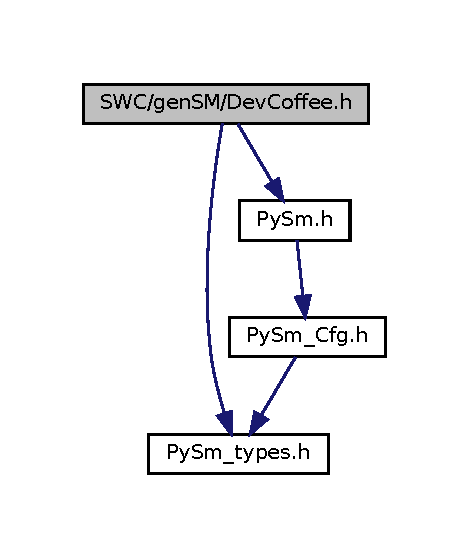
\includegraphics[width=225pt]{DevCoffee_8h__incl}
\end{center}
\end{figure}
This graph shows which files directly or indirectly include this file\+:
\nopagebreak
\begin{figure}[H]
\begin{center}
\leavevmode
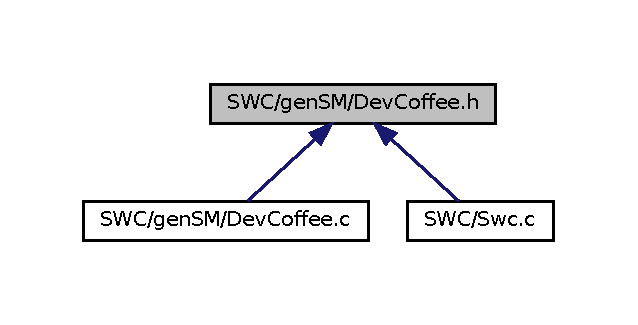
\includegraphics[width=306pt]{DevCoffee_8h__dep__incl}
\end{center}
\end{figure}
\subsection*{Data Structures}
\begin{DoxyCompactItemize}
\item 
struct \hyperlink{structdevCoffee__inputSignalsType}{dev\+Coffee\+\_\+input\+Signals\+Type}
\begin{DoxyCompactList}\small\item\em Structure defining input signals for state machine dev\+Coffee. \end{DoxyCompactList}\item 
struct \hyperlink{structdevCoffee__outputSignalsType}{dev\+Coffee\+\_\+output\+Signals\+Type}
\begin{DoxyCompactList}\small\item\em Structure defining output signals for state machine dev\+Coffee. \end{DoxyCompactList}\end{DoxyCompactItemize}
\subsection*{Macros}
\begin{DoxyCompactItemize}
\item 
\#define \hyperlink{DevCoffee_8h_aa1c96ba91026e5e8334b824647bbf313}{W\+O\+R\+K\+T\+I\+M\+E\+\_\+\+P\+E\+R\+\_\+\+D\+A\+Y\+\_\+H}~8
\item 
\#define \hyperlink{DevCoffee_8h_a11a09e9c07aa2d4de619e81fed6944bc}{W\+A\+K\+E\+\_\+\+U\+P\+\_\+\+T\+I\+M\+E\+\_\+H}~6 /$\ast$ stand up at 6 o\textquotesingle{}clock $\ast$/
\item 
\#define \hyperlink{DevCoffee_8h_a0dc8c99099d0b9caa0e8658967ccd201}{G\+O\+\_\+\+H\+O\+M\+E\+\_\+\+T\+I\+ME}~(\hyperlink{DevCoffee_8h_aa1c96ba91026e5e8334b824647bbf313}{W\+O\+R\+K\+T\+I\+M\+E\+\_\+\+P\+E\+R\+\_\+\+D\+A\+Y\+\_\+H}+\hyperlink{DevCoffee_8h_a11a09e9c07aa2d4de619e81fed6944bc}{W\+A\+K\+E\+\_\+\+U\+P\+\_\+\+T\+I\+M\+E\+\_\+H})
\end{DoxyCompactItemize}
\subsection*{Enumerations}
\begin{DoxyCompactItemize}
\item 
enum \hyperlink{DevCoffee_8h_a5590d50a72c7655d28dc92f0531c26dc}{dev\+Coffee\+\_\+active\+State\+Type} \{ \newline
\hyperlink{DevCoffee_8h_a5590d50a72c7655d28dc92f0531c26dca5c79ab73bc31ae6cd575cb28ce078adc}{dev\+Coffee\+\_\+\+U\+N\+I\+N\+I\+T\+A\+L\+I\+Z\+E\+D\+\_\+\+S\+T\+A\+T\+E\+\_\+\+M\+A\+C\+H\+I\+NE}, 
\hyperlink{DevCoffee_8h_a5590d50a72c7655d28dc92f0531c26dcaefe201d0581f045bde9ecf366aa79677}{D\+E\+V\+C\+O\+F\+F\+E\+E\+\_\+\+B\+R\+E\+A\+K\+F\+A\+ST}, 
\hyperlink{DevCoffee_8h_a5590d50a72c7655d28dc92f0531c26dca2a09ba1cf03d5d05523d3c4145c9f13d}{D\+E\+V\+C\+O\+F\+F\+E\+E\+\_\+\+I\+N\+\_\+\+O\+F\+F\+I\+CE}, 
\hyperlink{DevCoffee_8h_a5590d50a72c7655d28dc92f0531c26dca973ab37082032e99e9dc2d88713d9648}{D\+E\+V\+C\+O\+F\+F\+E\+E\+\_\+\+G\+E\+T\+\_\+\+C\+O\+F\+F\+EE}, 
\newline
\hyperlink{DevCoffee_8h_a5590d50a72c7655d28dc92f0531c26dcaf279a1642f76979556eeb02cc1c8add5}{D\+E\+V\+C\+O\+F\+F\+E\+E\+\_\+\+R\+E\+L\+A\+X\+\_\+\+A\+N\+D\+\_\+\+S\+L\+E\+EP}, 
\hyperlink{DevCoffee_8h_a5590d50a72c7655d28dc92f0531c26dca069ba7538574aadeb17b48e5449f9d72}{D\+E\+V\+C\+O\+F\+F\+E\+E\+\_\+\+D\+E\+V\+E\+L\+O\+P\+E\+R\+\_\+\+I\+S\+\_\+\+I\+LL}
 \}\begin{DoxyCompactList}\small\item\em Enum for exporting current active state of state machine dev\+Coffee. \end{DoxyCompactList}
\end{DoxyCompactItemize}
\subsection*{Functions}
\begin{DoxyCompactItemize}
\item 
\hyperlink{PySm_8h_a1bd760b7300136bf7e0bd7b9e3a126ff}{py\+Sm\+\_\+return\+Type} \hyperlink{DevCoffee_8h_a3a36c2b07e56da630d1932442bd41700}{Dev\+Coffee\+\_\+main\+Function} (\hyperlink{structdevCoffee__inputSignalsType}{dev\+Coffee\+\_\+input\+Signals\+Type} $\ast$, \hyperlink{structdevCoffee__outputSignalsType}{dev\+Coffee\+\_\+output\+Signals\+Type} $\ast$)
\begin{DoxyCompactList}\small\item\em Main function of the state machine dev\+Coffee. \end{DoxyCompactList}\item 
void \hyperlink{DevCoffee_8h_adefb739872826d1e12c496809d88918a}{Dev\+Coffee\+\_\+get\+Active\+State} (\hyperlink{DevCoffee_8h_a5590d50a72c7655d28dc92f0531c26dc}{dev\+Coffee\+\_\+active\+State\+Type} $\ast$)
\begin{DoxyCompactList}\small\item\em Main function of the state machine dev\+Coffee. \end{DoxyCompactList}\end{DoxyCompactItemize}


\subsection{Detailed Description}
Header for generated state machine dev\+Coffee Generated 2017-\/09-\/27 19\+:41\+:10 by Py\+SM -\/ The python state machine generator. 

\begin{DoxyAuthor}{Author}
Markus 
\end{DoxyAuthor}
\begin{DoxyDate}{Date}
2017-\/09-\/27 
\end{DoxyDate}


\subsection{Macro Definition Documentation}
\mbox{\Hypertarget{DevCoffee_8h_a0dc8c99099d0b9caa0e8658967ccd201}\label{DevCoffee_8h_a0dc8c99099d0b9caa0e8658967ccd201}} 
\index{Dev\+Coffee.\+h@{Dev\+Coffee.\+h}!G\+O\+\_\+\+H\+O\+M\+E\+\_\+\+T\+I\+ME@{G\+O\+\_\+\+H\+O\+M\+E\+\_\+\+T\+I\+ME}}
\index{G\+O\+\_\+\+H\+O\+M\+E\+\_\+\+T\+I\+ME@{G\+O\+\_\+\+H\+O\+M\+E\+\_\+\+T\+I\+ME}!Dev\+Coffee.\+h@{Dev\+Coffee.\+h}}
\subsubsection{\texorpdfstring{G\+O\+\_\+\+H\+O\+M\+E\+\_\+\+T\+I\+ME}{GO\_HOME\_TIME}}
{\footnotesize\ttfamily \#define G\+O\+\_\+\+H\+O\+M\+E\+\_\+\+T\+I\+ME~(\hyperlink{DevCoffee_8h_aa1c96ba91026e5e8334b824647bbf313}{W\+O\+R\+K\+T\+I\+M\+E\+\_\+\+P\+E\+R\+\_\+\+D\+A\+Y\+\_\+H}+\hyperlink{DevCoffee_8h_a11a09e9c07aa2d4de619e81fed6944bc}{W\+A\+K\+E\+\_\+\+U\+P\+\_\+\+T\+I\+M\+E\+\_\+H})}

\mbox{\Hypertarget{DevCoffee_8h_a11a09e9c07aa2d4de619e81fed6944bc}\label{DevCoffee_8h_a11a09e9c07aa2d4de619e81fed6944bc}} 
\index{Dev\+Coffee.\+h@{Dev\+Coffee.\+h}!W\+A\+K\+E\+\_\+\+U\+P\+\_\+\+T\+I\+M\+E\+\_\+H@{W\+A\+K\+E\+\_\+\+U\+P\+\_\+\+T\+I\+M\+E\+\_\+H}}
\index{W\+A\+K\+E\+\_\+\+U\+P\+\_\+\+T\+I\+M\+E\+\_\+H@{W\+A\+K\+E\+\_\+\+U\+P\+\_\+\+T\+I\+M\+E\+\_\+H}!Dev\+Coffee.\+h@{Dev\+Coffee.\+h}}
\subsubsection{\texorpdfstring{W\+A\+K\+E\+\_\+\+U\+P\+\_\+\+T\+I\+M\+E\+\_\+H}{WAKE\_UP\_TIME\_H}}
{\footnotesize\ttfamily \#define W\+A\+K\+E\+\_\+\+U\+P\+\_\+\+T\+I\+M\+E\+\_\+H~6 /$\ast$ stand up at 6 o\textquotesingle{}clock $\ast$/}

\mbox{\Hypertarget{DevCoffee_8h_aa1c96ba91026e5e8334b824647bbf313}\label{DevCoffee_8h_aa1c96ba91026e5e8334b824647bbf313}} 
\index{Dev\+Coffee.\+h@{Dev\+Coffee.\+h}!W\+O\+R\+K\+T\+I\+M\+E\+\_\+\+P\+E\+R\+\_\+\+D\+A\+Y\+\_\+H@{W\+O\+R\+K\+T\+I\+M\+E\+\_\+\+P\+E\+R\+\_\+\+D\+A\+Y\+\_\+H}}
\index{W\+O\+R\+K\+T\+I\+M\+E\+\_\+\+P\+E\+R\+\_\+\+D\+A\+Y\+\_\+H@{W\+O\+R\+K\+T\+I\+M\+E\+\_\+\+P\+E\+R\+\_\+\+D\+A\+Y\+\_\+H}!Dev\+Coffee.\+h@{Dev\+Coffee.\+h}}
\subsubsection{\texorpdfstring{W\+O\+R\+K\+T\+I\+M\+E\+\_\+\+P\+E\+R\+\_\+\+D\+A\+Y\+\_\+H}{WORKTIME\_PER\_DAY\_H}}
{\footnotesize\ttfamily \#define W\+O\+R\+K\+T\+I\+M\+E\+\_\+\+P\+E\+R\+\_\+\+D\+A\+Y\+\_\+H~8}



\subsection{Enumeration Type Documentation}
\mbox{\Hypertarget{DevCoffee_8h_a5590d50a72c7655d28dc92f0531c26dc}\label{DevCoffee_8h_a5590d50a72c7655d28dc92f0531c26dc}} 
\index{Dev\+Coffee.\+h@{Dev\+Coffee.\+h}!dev\+Coffee\+\_\+active\+State\+Type@{dev\+Coffee\+\_\+active\+State\+Type}}
\index{dev\+Coffee\+\_\+active\+State\+Type@{dev\+Coffee\+\_\+active\+State\+Type}!Dev\+Coffee.\+h@{Dev\+Coffee.\+h}}
\subsubsection{\texorpdfstring{dev\+Coffee\+\_\+active\+State\+Type}{devCoffee\_activeStateType}}
{\footnotesize\ttfamily enum \hyperlink{DevCoffee_8h_a5590d50a72c7655d28dc92f0531c26dc}{dev\+Coffee\+\_\+active\+State\+Type}}



Enum for exporting current active state of state machine dev\+Coffee. 

\begin{DoxyEnumFields}{Enumerator}
\raisebox{\heightof{T}}[0pt][0pt]{\index{dev\+Coffee\+\_\+\+U\+N\+I\+N\+I\+T\+A\+L\+I\+Z\+E\+D\+\_\+\+S\+T\+A\+T\+E\+\_\+\+M\+A\+C\+H\+I\+NE@{dev\+Coffee\+\_\+\+U\+N\+I\+N\+I\+T\+A\+L\+I\+Z\+E\+D\+\_\+\+S\+T\+A\+T\+E\+\_\+\+M\+A\+C\+H\+I\+NE}!Dev\+Coffee.\+h@{Dev\+Coffee.\+h}}\index{Dev\+Coffee.\+h@{Dev\+Coffee.\+h}!dev\+Coffee\+\_\+\+U\+N\+I\+N\+I\+T\+A\+L\+I\+Z\+E\+D\+\_\+\+S\+T\+A\+T\+E\+\_\+\+M\+A\+C\+H\+I\+NE@{dev\+Coffee\+\_\+\+U\+N\+I\+N\+I\+T\+A\+L\+I\+Z\+E\+D\+\_\+\+S\+T\+A\+T\+E\+\_\+\+M\+A\+C\+H\+I\+NE}}}\mbox{\Hypertarget{DevCoffee_8h_a5590d50a72c7655d28dc92f0531c26dca5c79ab73bc31ae6cd575cb28ce078adc}\label{DevCoffee_8h_a5590d50a72c7655d28dc92f0531c26dca5c79ab73bc31ae6cd575cb28ce078adc}} 
dev\+Coffee\+\_\+\+U\+N\+I\+N\+I\+T\+A\+L\+I\+Z\+E\+D\+\_\+\+S\+T\+A\+T\+E\+\_\+\+M\+A\+C\+H\+I\+NE&\\
\hline

\raisebox{\heightof{T}}[0pt][0pt]{\index{D\+E\+V\+C\+O\+F\+F\+E\+E\+\_\+\+B\+R\+E\+A\+K\+F\+A\+ST@{D\+E\+V\+C\+O\+F\+F\+E\+E\+\_\+\+B\+R\+E\+A\+K\+F\+A\+ST}!Dev\+Coffee.\+h@{Dev\+Coffee.\+h}}\index{Dev\+Coffee.\+h@{Dev\+Coffee.\+h}!D\+E\+V\+C\+O\+F\+F\+E\+E\+\_\+\+B\+R\+E\+A\+K\+F\+A\+ST@{D\+E\+V\+C\+O\+F\+F\+E\+E\+\_\+\+B\+R\+E\+A\+K\+F\+A\+ST}}}\mbox{\Hypertarget{DevCoffee_8h_a5590d50a72c7655d28dc92f0531c26dcaefe201d0581f045bde9ecf366aa79677}\label{DevCoffee_8h_a5590d50a72c7655d28dc92f0531c26dcaefe201d0581f045bde9ecf366aa79677}} 
D\+E\+V\+C\+O\+F\+F\+E\+E\+\_\+\+B\+R\+E\+A\+K\+F\+A\+ST&\\
\hline

\raisebox{\heightof{T}}[0pt][0pt]{\index{D\+E\+V\+C\+O\+F\+F\+E\+E\+\_\+\+I\+N\+\_\+\+O\+F\+F\+I\+CE@{D\+E\+V\+C\+O\+F\+F\+E\+E\+\_\+\+I\+N\+\_\+\+O\+F\+F\+I\+CE}!Dev\+Coffee.\+h@{Dev\+Coffee.\+h}}\index{Dev\+Coffee.\+h@{Dev\+Coffee.\+h}!D\+E\+V\+C\+O\+F\+F\+E\+E\+\_\+\+I\+N\+\_\+\+O\+F\+F\+I\+CE@{D\+E\+V\+C\+O\+F\+F\+E\+E\+\_\+\+I\+N\+\_\+\+O\+F\+F\+I\+CE}}}\mbox{\Hypertarget{DevCoffee_8h_a5590d50a72c7655d28dc92f0531c26dca2a09ba1cf03d5d05523d3c4145c9f13d}\label{DevCoffee_8h_a5590d50a72c7655d28dc92f0531c26dca2a09ba1cf03d5d05523d3c4145c9f13d}} 
D\+E\+V\+C\+O\+F\+F\+E\+E\+\_\+\+I\+N\+\_\+\+O\+F\+F\+I\+CE&\\
\hline

\raisebox{\heightof{T}}[0pt][0pt]{\index{D\+E\+V\+C\+O\+F\+F\+E\+E\+\_\+\+G\+E\+T\+\_\+\+C\+O\+F\+F\+EE@{D\+E\+V\+C\+O\+F\+F\+E\+E\+\_\+\+G\+E\+T\+\_\+\+C\+O\+F\+F\+EE}!Dev\+Coffee.\+h@{Dev\+Coffee.\+h}}\index{Dev\+Coffee.\+h@{Dev\+Coffee.\+h}!D\+E\+V\+C\+O\+F\+F\+E\+E\+\_\+\+G\+E\+T\+\_\+\+C\+O\+F\+F\+EE@{D\+E\+V\+C\+O\+F\+F\+E\+E\+\_\+\+G\+E\+T\+\_\+\+C\+O\+F\+F\+EE}}}\mbox{\Hypertarget{DevCoffee_8h_a5590d50a72c7655d28dc92f0531c26dca973ab37082032e99e9dc2d88713d9648}\label{DevCoffee_8h_a5590d50a72c7655d28dc92f0531c26dca973ab37082032e99e9dc2d88713d9648}} 
D\+E\+V\+C\+O\+F\+F\+E\+E\+\_\+\+G\+E\+T\+\_\+\+C\+O\+F\+F\+EE&\\
\hline

\raisebox{\heightof{T}}[0pt][0pt]{\index{D\+E\+V\+C\+O\+F\+F\+E\+E\+\_\+\+R\+E\+L\+A\+X\+\_\+\+A\+N\+D\+\_\+\+S\+L\+E\+EP@{D\+E\+V\+C\+O\+F\+F\+E\+E\+\_\+\+R\+E\+L\+A\+X\+\_\+\+A\+N\+D\+\_\+\+S\+L\+E\+EP}!Dev\+Coffee.\+h@{Dev\+Coffee.\+h}}\index{Dev\+Coffee.\+h@{Dev\+Coffee.\+h}!D\+E\+V\+C\+O\+F\+F\+E\+E\+\_\+\+R\+E\+L\+A\+X\+\_\+\+A\+N\+D\+\_\+\+S\+L\+E\+EP@{D\+E\+V\+C\+O\+F\+F\+E\+E\+\_\+\+R\+E\+L\+A\+X\+\_\+\+A\+N\+D\+\_\+\+S\+L\+E\+EP}}}\mbox{\Hypertarget{DevCoffee_8h_a5590d50a72c7655d28dc92f0531c26dcaf279a1642f76979556eeb02cc1c8add5}\label{DevCoffee_8h_a5590d50a72c7655d28dc92f0531c26dcaf279a1642f76979556eeb02cc1c8add5}} 
D\+E\+V\+C\+O\+F\+F\+E\+E\+\_\+\+R\+E\+L\+A\+X\+\_\+\+A\+N\+D\+\_\+\+S\+L\+E\+EP&\\
\hline

\raisebox{\heightof{T}}[0pt][0pt]{\index{D\+E\+V\+C\+O\+F\+F\+E\+E\+\_\+\+D\+E\+V\+E\+L\+O\+P\+E\+R\+\_\+\+I\+S\+\_\+\+I\+LL@{D\+E\+V\+C\+O\+F\+F\+E\+E\+\_\+\+D\+E\+V\+E\+L\+O\+P\+E\+R\+\_\+\+I\+S\+\_\+\+I\+LL}!Dev\+Coffee.\+h@{Dev\+Coffee.\+h}}\index{Dev\+Coffee.\+h@{Dev\+Coffee.\+h}!D\+E\+V\+C\+O\+F\+F\+E\+E\+\_\+\+D\+E\+V\+E\+L\+O\+P\+E\+R\+\_\+\+I\+S\+\_\+\+I\+LL@{D\+E\+V\+C\+O\+F\+F\+E\+E\+\_\+\+D\+E\+V\+E\+L\+O\+P\+E\+R\+\_\+\+I\+S\+\_\+\+I\+LL}}}\mbox{\Hypertarget{DevCoffee_8h_a5590d50a72c7655d28dc92f0531c26dca069ba7538574aadeb17b48e5449f9d72}\label{DevCoffee_8h_a5590d50a72c7655d28dc92f0531c26dca069ba7538574aadeb17b48e5449f9d72}} 
D\+E\+V\+C\+O\+F\+F\+E\+E\+\_\+\+D\+E\+V\+E\+L\+O\+P\+E\+R\+\_\+\+I\+S\+\_\+\+I\+LL&\\
\hline

\end{DoxyEnumFields}


\subsection{Function Documentation}
\mbox{\Hypertarget{DevCoffee_8h_adefb739872826d1e12c496809d88918a}\label{DevCoffee_8h_adefb739872826d1e12c496809d88918a}} 
\index{Dev\+Coffee.\+h@{Dev\+Coffee.\+h}!Dev\+Coffee\+\_\+get\+Active\+State@{Dev\+Coffee\+\_\+get\+Active\+State}}
\index{Dev\+Coffee\+\_\+get\+Active\+State@{Dev\+Coffee\+\_\+get\+Active\+State}!Dev\+Coffee.\+h@{Dev\+Coffee.\+h}}
\subsubsection{\texorpdfstring{Dev\+Coffee\+\_\+get\+Active\+State()}{DevCoffee\_getActiveState()}}
{\footnotesize\ttfamily void Dev\+Coffee\+\_\+get\+Active\+State (\begin{DoxyParamCaption}\item[{\hyperlink{DevCoffee_8h_a5590d50a72c7655d28dc92f0531c26dc}{dev\+Coffee\+\_\+active\+State\+Type} $\ast$}]{ }\end{DoxyParamCaption})}



Main function of the state machine dev\+Coffee. 

\mbox{\Hypertarget{DevCoffee_8h_a3a36c2b07e56da630d1932442bd41700}\label{DevCoffee_8h_a3a36c2b07e56da630d1932442bd41700}} 
\index{Dev\+Coffee.\+h@{Dev\+Coffee.\+h}!Dev\+Coffee\+\_\+main\+Function@{Dev\+Coffee\+\_\+main\+Function}}
\index{Dev\+Coffee\+\_\+main\+Function@{Dev\+Coffee\+\_\+main\+Function}!Dev\+Coffee.\+h@{Dev\+Coffee.\+h}}
\subsubsection{\texorpdfstring{Dev\+Coffee\+\_\+main\+Function()}{DevCoffee\_mainFunction()}}
{\footnotesize\ttfamily \hyperlink{PySm_8h_a1bd760b7300136bf7e0bd7b9e3a126ff}{py\+Sm\+\_\+return\+Type} Dev\+Coffee\+\_\+main\+Function (\begin{DoxyParamCaption}\item[{\hyperlink{structdevCoffee__inputSignalsType}{dev\+Coffee\+\_\+input\+Signals\+Type} $\ast$}]{,  }\item[{\hyperlink{structdevCoffee__outputSignalsType}{dev\+Coffee\+\_\+output\+Signals\+Type} $\ast$}]{ }\end{DoxyParamCaption})}



Main function of the state machine dev\+Coffee. 

Here is the call graph for this function\+:\nopagebreak
\begin{figure}[H]
\begin{center}
\leavevmode
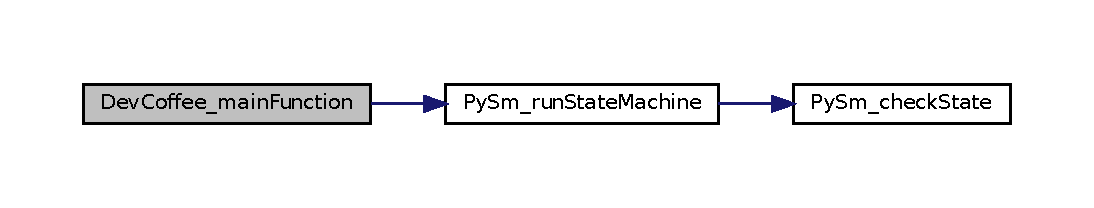
\includegraphics[width=350pt]{DevCoffee_8h_a3a36c2b07e56da630d1932442bd41700_cgraph}
\end{center}
\end{figure}

\hypertarget{SimpleEx_8c}{}\section{S\+W\+C/gen\+S\+M/\+Simple\+Ex.c File Reference}
\label{SimpleEx_8c}\index{S\+W\+C/gen\+S\+M/\+Simple\+Ex.\+c@{S\+W\+C/gen\+S\+M/\+Simple\+Ex.\+c}}


Header for generated state machine simple\+Ex Generated 2017-\/11-\/04 13\+:36\+:42 by Py\+SM -\/ The python state machine generator.  


{\ttfamily \#include \char`\"{}Simple\+Ex.\+h\char`\"{}}\newline
Include dependency graph for Simple\+Ex.\+c\+:
\nopagebreak
\begin{figure}[H]
\begin{center}
\leavevmode
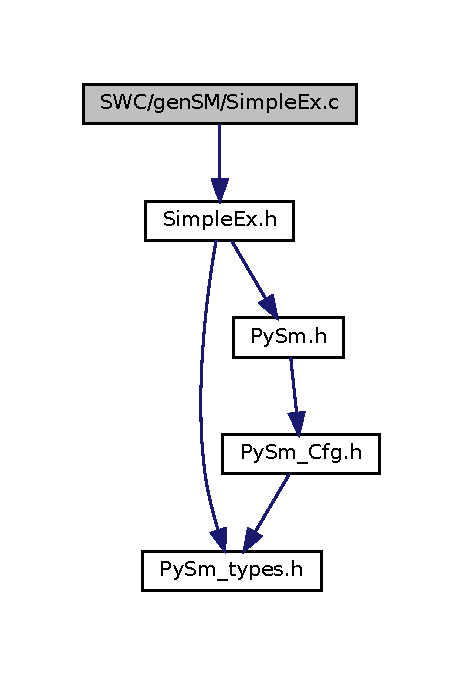
\includegraphics[width=222pt]{SimpleEx_8c__incl}
\end{center}
\end{figure}
\subsection*{Functions}
\begin{DoxyCompactItemize}
\item 
static void \hyperlink{SimpleEx_8c_a35c76636dcdd303ca1f3fdfb66446464}{simple\+Ex\+\_\+\+S\+F\+\_\+state1\+\_\+entry} (void)
\item 
static void \hyperlink{SimpleEx_8c_aaa2ce8029b0667fe30bb70d8aade0be7}{simple\+Ex\+\_\+\+S\+F\+\_\+state2\+\_\+entry} (void)
\item 
static void \hyperlink{SimpleEx_8c_ae3507e06080e7fd0ca26a589e8c4ce07}{simple\+Ex\+\_\+\+S\+F\+\_\+state2} (void)
\item 
static void \hyperlink{SimpleEx_8c_a2a33585c697124c651c84778569a7989}{simple\+Ex\+\_\+\+S\+F\+\_\+state3\+\_\+entry} (void)
\item 
static void \hyperlink{SimpleEx_8c_a910d670f2661b056c32b541341a74305}{simple\+Ex\+\_\+\+S\+F\+\_\+state3\+\_\+exit} (void)
\item 
static void \hyperlink{SimpleEx_8c_ab0ed369d92b9d015715fa70409045d46}{simple\+Ex\+\_\+variable\+Reset\+Function} (void)
\item 
\hyperlink{PySm_8h_a1bd760b7300136bf7e0bd7b9e3a126ff}{py\+Sm\+\_\+return\+Type} \hyperlink{SimpleEx_8c_aa6374857abc588e169064d2f89a0a3e0}{Simple\+Ex\+\_\+main\+Function} (void)
\begin{DoxyCompactList}\small\item\em Main function of the state machine simple\+Ex. \end{DoxyCompactList}\item 
void \hyperlink{SimpleEx_8c_a4a3771cce61cff507afb4a6925e5e87e}{Simple\+Ex\+\_\+get\+Active\+State} (\hyperlink{SimpleEx_8h_adaa7d471cac739753efb6254f6f039e5}{simple\+Ex\+\_\+active\+State\+Type} $\ast$swc\+\_\+active\+State)
\begin{DoxyCompactList}\small\item\em Main function of the state machine simple\+Ex. \end{DoxyCompactList}\end{DoxyCompactItemize}
\subsection*{Variables}
\begin{DoxyCompactItemize}
\item 
static const \hyperlink{structpySm__stateType}{py\+Sm\+\_\+state\+Type} \hyperlink{SimpleEx_8c_af6cf222808cf96c1266e8cb31c0b4490}{simple\+Ex\+\_\+state\+\_\+state1}
\item 
static const \hyperlink{structpySm__stateType}{py\+Sm\+\_\+state\+Type} \hyperlink{SimpleEx_8c_a6bf0b5b4eaa4c5c6bda5f7892625e6c8}{simple\+Ex\+\_\+state\+\_\+state2}
\item 
static const \hyperlink{structpySm__stateType}{py\+Sm\+\_\+state\+Type} \hyperlink{SimpleEx_8c_af9bc491df98b7873ce0b0477c398688c}{simple\+Ex\+\_\+state\+\_\+state3}
\item 
static const \hyperlink{structpySm__stateType}{py\+Sm\+\_\+state\+Type} $\ast$ \hyperlink{SimpleEx_8c_ad65d2cd3836e521d59fb04c71e718b61}{simple\+Ex\+\_\+states\+\_\+pa} \mbox{[}3\mbox{]}
\item 
static \hyperlink{structpySm__stateTransitionType}{py\+Sm\+\_\+state\+Transition\+Type} \hyperlink{SimpleEx_8c_a2cdd50d897d203f7865b5976a2e9c65a}{simple\+Ex\+\_\+transitions\+\_\+sa} \mbox{[}3\mbox{]}
\item 
\hyperlink{structpySm__stateMachineType}{py\+Sm\+\_\+state\+Machine\+Type} \hyperlink{SimpleEx_8c_a755a38d37164be4d7fa5c091d3fa9b58}{simple\+Ex\+\_\+state\+Machine\+\_\+s}
\item 
static \hyperlink{SimpleEx_8h_adaa7d471cac739753efb6254f6f039e5}{simple\+Ex\+\_\+active\+State\+Type} \hyperlink{SimpleEx_8c_a29ff66e876b3a41b2564b673a6a9dcb5}{simple\+Ex\+\_\+active\+State} = \hyperlink{SimpleEx_8h_adaa7d471cac739753efb6254f6f039e5acaffc5763218f7c0b9f77c62754ee635}{S\+I\+M\+P\+L\+E\+E\+X\+\_\+\+U\+N\+I\+N\+I\+T\+A\+L\+I\+Z\+E\+D\+\_\+\+S\+T\+A\+T\+E\+\_\+\+M\+A\+C\+H\+I\+NE}
\item 
\hyperlink{PySm__types_8h_a1aff40256c00f194609879f8f6f1e1a1}{py\+Sm\+\_\+uint8} \hyperlink{SimpleEx_8c_a91db4bf981a46cbe3422da2e6ddff3df}{local\+\_\+variable\+\_\+ui8} = 0u
\end{DoxyCompactItemize}


\subsection{Detailed Description}
Header for generated state machine simple\+Ex Generated 2017-\/11-\/04 13\+:36\+:42 by Py\+SM -\/ The python state machine generator. 

\begin{DoxyAuthor}{Author}
Markus Burger 
\end{DoxyAuthor}
\begin{DoxyDate}{Date}
2017-\/11-\/04 
\end{DoxyDate}


\subsection{Function Documentation}
\mbox{\Hypertarget{SimpleEx_8c_a4a3771cce61cff507afb4a6925e5e87e}\label{SimpleEx_8c_a4a3771cce61cff507afb4a6925e5e87e}} 
\index{Simple\+Ex.\+c@{Simple\+Ex.\+c}!Simple\+Ex\+\_\+get\+Active\+State@{Simple\+Ex\+\_\+get\+Active\+State}}
\index{Simple\+Ex\+\_\+get\+Active\+State@{Simple\+Ex\+\_\+get\+Active\+State}!Simple\+Ex.\+c@{Simple\+Ex.\+c}}
\subsubsection{\texorpdfstring{Simple\+Ex\+\_\+get\+Active\+State()}{SimpleEx\_getActiveState()}}
{\footnotesize\ttfamily void Simple\+Ex\+\_\+get\+Active\+State (\begin{DoxyParamCaption}\item[{\hyperlink{SimpleEx_8h_adaa7d471cac739753efb6254f6f039e5}{simple\+Ex\+\_\+active\+State\+Type} $\ast$}]{swc\+\_\+active\+State }\end{DoxyParamCaption})}



Main function of the state machine simple\+Ex. 

\mbox{\Hypertarget{SimpleEx_8c_aa6374857abc588e169064d2f89a0a3e0}\label{SimpleEx_8c_aa6374857abc588e169064d2f89a0a3e0}} 
\index{Simple\+Ex.\+c@{Simple\+Ex.\+c}!Simple\+Ex\+\_\+main\+Function@{Simple\+Ex\+\_\+main\+Function}}
\index{Simple\+Ex\+\_\+main\+Function@{Simple\+Ex\+\_\+main\+Function}!Simple\+Ex.\+c@{Simple\+Ex.\+c}}
\subsubsection{\texorpdfstring{Simple\+Ex\+\_\+main\+Function()}{SimpleEx\_mainFunction()}}
{\footnotesize\ttfamily \hyperlink{PySm_8h_a1bd760b7300136bf7e0bd7b9e3a126ff}{py\+Sm\+\_\+return\+Type} Simple\+Ex\+\_\+main\+Function (\begin{DoxyParamCaption}\item[{void}]{ }\end{DoxyParamCaption})}



Main function of the state machine simple\+Ex. 

Here is the call graph for this function\+:
\nopagebreak
\begin{figure}[H]
\begin{center}
\leavevmode
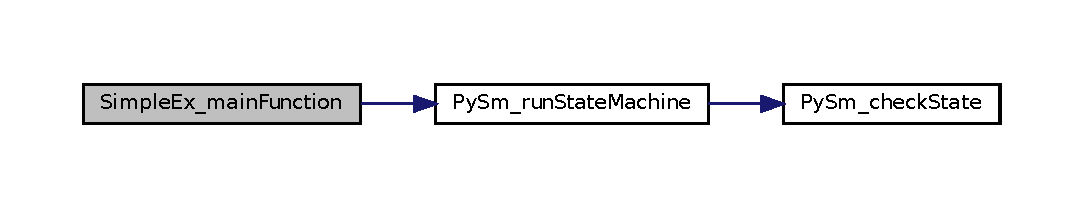
\includegraphics[width=350pt]{SimpleEx_8c_aa6374857abc588e169064d2f89a0a3e0_cgraph}
\end{center}
\end{figure}
\mbox{\Hypertarget{SimpleEx_8c_a35c76636dcdd303ca1f3fdfb66446464}\label{SimpleEx_8c_a35c76636dcdd303ca1f3fdfb66446464}} 
\index{Simple\+Ex.\+c@{Simple\+Ex.\+c}!simple\+Ex\+\_\+\+S\+F\+\_\+state1\+\_\+entry@{simple\+Ex\+\_\+\+S\+F\+\_\+state1\+\_\+entry}}
\index{simple\+Ex\+\_\+\+S\+F\+\_\+state1\+\_\+entry@{simple\+Ex\+\_\+\+S\+F\+\_\+state1\+\_\+entry}!Simple\+Ex.\+c@{Simple\+Ex.\+c}}
\subsubsection{\texorpdfstring{simple\+Ex\+\_\+\+S\+F\+\_\+state1\+\_\+entry()}{simpleEx\_SF\_state1\_entry()}}
{\footnotesize\ttfamily static void simple\+Ex\+\_\+\+S\+F\+\_\+state1\+\_\+entry (\begin{DoxyParamCaption}\item[{void}]{ }\end{DoxyParamCaption})\hspace{0.3cm}{\ttfamily [static]}}

\mbox{\Hypertarget{SimpleEx_8c_ae3507e06080e7fd0ca26a589e8c4ce07}\label{SimpleEx_8c_ae3507e06080e7fd0ca26a589e8c4ce07}} 
\index{Simple\+Ex.\+c@{Simple\+Ex.\+c}!simple\+Ex\+\_\+\+S\+F\+\_\+state2@{simple\+Ex\+\_\+\+S\+F\+\_\+state2}}
\index{simple\+Ex\+\_\+\+S\+F\+\_\+state2@{simple\+Ex\+\_\+\+S\+F\+\_\+state2}!Simple\+Ex.\+c@{Simple\+Ex.\+c}}
\subsubsection{\texorpdfstring{simple\+Ex\+\_\+\+S\+F\+\_\+state2()}{simpleEx\_SF\_state2()}}
{\footnotesize\ttfamily static void simple\+Ex\+\_\+\+S\+F\+\_\+state2 (\begin{DoxyParamCaption}\item[{void}]{ }\end{DoxyParamCaption})\hspace{0.3cm}{\ttfamily [static]}}

\mbox{\Hypertarget{SimpleEx_8c_aaa2ce8029b0667fe30bb70d8aade0be7}\label{SimpleEx_8c_aaa2ce8029b0667fe30bb70d8aade0be7}} 
\index{Simple\+Ex.\+c@{Simple\+Ex.\+c}!simple\+Ex\+\_\+\+S\+F\+\_\+state2\+\_\+entry@{simple\+Ex\+\_\+\+S\+F\+\_\+state2\+\_\+entry}}
\index{simple\+Ex\+\_\+\+S\+F\+\_\+state2\+\_\+entry@{simple\+Ex\+\_\+\+S\+F\+\_\+state2\+\_\+entry}!Simple\+Ex.\+c@{Simple\+Ex.\+c}}
\subsubsection{\texorpdfstring{simple\+Ex\+\_\+\+S\+F\+\_\+state2\+\_\+entry()}{simpleEx\_SF\_state2\_entry()}}
{\footnotesize\ttfamily static void simple\+Ex\+\_\+\+S\+F\+\_\+state2\+\_\+entry (\begin{DoxyParamCaption}\item[{void}]{ }\end{DoxyParamCaption})\hspace{0.3cm}{\ttfamily [static]}}

\mbox{\Hypertarget{SimpleEx_8c_a2a33585c697124c651c84778569a7989}\label{SimpleEx_8c_a2a33585c697124c651c84778569a7989}} 
\index{Simple\+Ex.\+c@{Simple\+Ex.\+c}!simple\+Ex\+\_\+\+S\+F\+\_\+state3\+\_\+entry@{simple\+Ex\+\_\+\+S\+F\+\_\+state3\+\_\+entry}}
\index{simple\+Ex\+\_\+\+S\+F\+\_\+state3\+\_\+entry@{simple\+Ex\+\_\+\+S\+F\+\_\+state3\+\_\+entry}!Simple\+Ex.\+c@{Simple\+Ex.\+c}}
\subsubsection{\texorpdfstring{simple\+Ex\+\_\+\+S\+F\+\_\+state3\+\_\+entry()}{simpleEx\_SF\_state3\_entry()}}
{\footnotesize\ttfamily static void simple\+Ex\+\_\+\+S\+F\+\_\+state3\+\_\+entry (\begin{DoxyParamCaption}\item[{void}]{ }\end{DoxyParamCaption})\hspace{0.3cm}{\ttfamily [static]}}

\mbox{\Hypertarget{SimpleEx_8c_a910d670f2661b056c32b541341a74305}\label{SimpleEx_8c_a910d670f2661b056c32b541341a74305}} 
\index{Simple\+Ex.\+c@{Simple\+Ex.\+c}!simple\+Ex\+\_\+\+S\+F\+\_\+state3\+\_\+exit@{simple\+Ex\+\_\+\+S\+F\+\_\+state3\+\_\+exit}}
\index{simple\+Ex\+\_\+\+S\+F\+\_\+state3\+\_\+exit@{simple\+Ex\+\_\+\+S\+F\+\_\+state3\+\_\+exit}!Simple\+Ex.\+c@{Simple\+Ex.\+c}}
\subsubsection{\texorpdfstring{simple\+Ex\+\_\+\+S\+F\+\_\+state3\+\_\+exit()}{simpleEx\_SF\_state3\_exit()}}
{\footnotesize\ttfamily static void simple\+Ex\+\_\+\+S\+F\+\_\+state3\+\_\+exit (\begin{DoxyParamCaption}\item[{void}]{ }\end{DoxyParamCaption})\hspace{0.3cm}{\ttfamily [static]}}

\mbox{\Hypertarget{SimpleEx_8c_ab0ed369d92b9d015715fa70409045d46}\label{SimpleEx_8c_ab0ed369d92b9d015715fa70409045d46}} 
\index{Simple\+Ex.\+c@{Simple\+Ex.\+c}!simple\+Ex\+\_\+variable\+Reset\+Function@{simple\+Ex\+\_\+variable\+Reset\+Function}}
\index{simple\+Ex\+\_\+variable\+Reset\+Function@{simple\+Ex\+\_\+variable\+Reset\+Function}!Simple\+Ex.\+c@{Simple\+Ex.\+c}}
\subsubsection{\texorpdfstring{simple\+Ex\+\_\+variable\+Reset\+Function()}{simpleEx\_variableResetFunction()}}
{\footnotesize\ttfamily static void simple\+Ex\+\_\+variable\+Reset\+Function (\begin{DoxyParamCaption}\item[{void}]{ }\end{DoxyParamCaption})\hspace{0.3cm}{\ttfamily [static]}}



\subsection{Variable Documentation}
\mbox{\Hypertarget{SimpleEx_8c_a91db4bf981a46cbe3422da2e6ddff3df}\label{SimpleEx_8c_a91db4bf981a46cbe3422da2e6ddff3df}} 
\index{Simple\+Ex.\+c@{Simple\+Ex.\+c}!local\+\_\+variable\+\_\+ui8@{local\+\_\+variable\+\_\+ui8}}
\index{local\+\_\+variable\+\_\+ui8@{local\+\_\+variable\+\_\+ui8}!Simple\+Ex.\+c@{Simple\+Ex.\+c}}
\subsubsection{\texorpdfstring{local\+\_\+variable\+\_\+ui8}{local\_variable\_ui8}}
{\footnotesize\ttfamily \hyperlink{PySm__types_8h_a1aff40256c00f194609879f8f6f1e1a1}{py\+Sm\+\_\+uint8} local\+\_\+variable\+\_\+ui8 = 0u}

\mbox{\Hypertarget{SimpleEx_8c_a29ff66e876b3a41b2564b673a6a9dcb5}\label{SimpleEx_8c_a29ff66e876b3a41b2564b673a6a9dcb5}} 
\index{Simple\+Ex.\+c@{Simple\+Ex.\+c}!simple\+Ex\+\_\+active\+State@{simple\+Ex\+\_\+active\+State}}
\index{simple\+Ex\+\_\+active\+State@{simple\+Ex\+\_\+active\+State}!Simple\+Ex.\+c@{Simple\+Ex.\+c}}
\subsubsection{\texorpdfstring{simple\+Ex\+\_\+active\+State}{simpleEx\_activeState}}
{\footnotesize\ttfamily \hyperlink{SimpleEx_8h_adaa7d471cac739753efb6254f6f039e5}{simple\+Ex\+\_\+active\+State\+Type} simple\+Ex\+\_\+active\+State = \hyperlink{SimpleEx_8h_adaa7d471cac739753efb6254f6f039e5acaffc5763218f7c0b9f77c62754ee635}{S\+I\+M\+P\+L\+E\+E\+X\+\_\+\+U\+N\+I\+N\+I\+T\+A\+L\+I\+Z\+E\+D\+\_\+\+S\+T\+A\+T\+E\+\_\+\+M\+A\+C\+H\+I\+NE}\hspace{0.3cm}{\ttfamily [static]}}

\mbox{\Hypertarget{SimpleEx_8c_af6cf222808cf96c1266e8cb31c0b4490}\label{SimpleEx_8c_af6cf222808cf96c1266e8cb31c0b4490}} 
\index{Simple\+Ex.\+c@{Simple\+Ex.\+c}!simple\+Ex\+\_\+state\+\_\+state1@{simple\+Ex\+\_\+state\+\_\+state1}}
\index{simple\+Ex\+\_\+state\+\_\+state1@{simple\+Ex\+\_\+state\+\_\+state1}!Simple\+Ex.\+c@{Simple\+Ex.\+c}}
\subsubsection{\texorpdfstring{simple\+Ex\+\_\+state\+\_\+state1}{simpleEx\_state\_state1}}
{\footnotesize\ttfamily const \hyperlink{structpySm__stateType}{py\+Sm\+\_\+state\+Type} simple\+Ex\+\_\+state\+\_\+state1\hspace{0.3cm}{\ttfamily [static]}}

{\bfseries Initial value\+:}
\begin{DoxyCode}
=
\{
        .onEntryState = \hyperlink{SimpleEx_8c_a35c76636dcdd303ca1f3fdfb66446464}{simpleEx\_SF\_state1\_entry},
        .onState = \hyperlink{PySm__types_8h_a2afdb5c4ce56548232a74e689113cb95}{PYSM\_NULL\_PTR},
        .onExitState = \hyperlink{PySm__types_8h_a2afdb5c4ce56548232a74e689113cb95}{PYSM\_NULL\_PTR}
\}
\end{DoxyCode}
\mbox{\Hypertarget{SimpleEx_8c_a6bf0b5b4eaa4c5c6bda5f7892625e6c8}\label{SimpleEx_8c_a6bf0b5b4eaa4c5c6bda5f7892625e6c8}} 
\index{Simple\+Ex.\+c@{Simple\+Ex.\+c}!simple\+Ex\+\_\+state\+\_\+state2@{simple\+Ex\+\_\+state\+\_\+state2}}
\index{simple\+Ex\+\_\+state\+\_\+state2@{simple\+Ex\+\_\+state\+\_\+state2}!Simple\+Ex.\+c@{Simple\+Ex.\+c}}
\subsubsection{\texorpdfstring{simple\+Ex\+\_\+state\+\_\+state2}{simpleEx\_state\_state2}}
{\footnotesize\ttfamily const \hyperlink{structpySm__stateType}{py\+Sm\+\_\+state\+Type} simple\+Ex\+\_\+state\+\_\+state2\hspace{0.3cm}{\ttfamily [static]}}

{\bfseries Initial value\+:}
\begin{DoxyCode}
=
\{
        .onEntryState = \hyperlink{SimpleEx_8c_aaa2ce8029b0667fe30bb70d8aade0be7}{simpleEx\_SF\_state2\_entry},
        .onState = \hyperlink{SimpleEx_8c_ae3507e06080e7fd0ca26a589e8c4ce07}{simpleEx\_SF\_state2},
        .onExitState = \hyperlink{PySm__types_8h_a2afdb5c4ce56548232a74e689113cb95}{PYSM\_NULL\_PTR}
\}
\end{DoxyCode}
\mbox{\Hypertarget{SimpleEx_8c_af9bc491df98b7873ce0b0477c398688c}\label{SimpleEx_8c_af9bc491df98b7873ce0b0477c398688c}} 
\index{Simple\+Ex.\+c@{Simple\+Ex.\+c}!simple\+Ex\+\_\+state\+\_\+state3@{simple\+Ex\+\_\+state\+\_\+state3}}
\index{simple\+Ex\+\_\+state\+\_\+state3@{simple\+Ex\+\_\+state\+\_\+state3}!Simple\+Ex.\+c@{Simple\+Ex.\+c}}
\subsubsection{\texorpdfstring{simple\+Ex\+\_\+state\+\_\+state3}{simpleEx\_state\_state3}}
{\footnotesize\ttfamily const \hyperlink{structpySm__stateType}{py\+Sm\+\_\+state\+Type} simple\+Ex\+\_\+state\+\_\+state3\hspace{0.3cm}{\ttfamily [static]}}

{\bfseries Initial value\+:}
\begin{DoxyCode}
=
\{
        .onEntryState = \hyperlink{SimpleEx_8c_a2a33585c697124c651c84778569a7989}{simpleEx\_SF\_state3\_entry},
        .onState = \hyperlink{PySm__types_8h_a2afdb5c4ce56548232a74e689113cb95}{PYSM\_NULL\_PTR},
        .onExitState = \hyperlink{SimpleEx_8c_a910d670f2661b056c32b541341a74305}{simpleEx\_SF\_state3\_exit}
\}
\end{DoxyCode}
\mbox{\Hypertarget{SimpleEx_8c_a755a38d37164be4d7fa5c091d3fa9b58}\label{SimpleEx_8c_a755a38d37164be4d7fa5c091d3fa9b58}} 
\index{Simple\+Ex.\+c@{Simple\+Ex.\+c}!simple\+Ex\+\_\+state\+Machine\+\_\+s@{simple\+Ex\+\_\+state\+Machine\+\_\+s}}
\index{simple\+Ex\+\_\+state\+Machine\+\_\+s@{simple\+Ex\+\_\+state\+Machine\+\_\+s}!Simple\+Ex.\+c@{Simple\+Ex.\+c}}
\subsubsection{\texorpdfstring{simple\+Ex\+\_\+state\+Machine\+\_\+s}{simpleEx\_stateMachine\_s}}
{\footnotesize\ttfamily \hyperlink{structpySm__stateMachineType}{py\+Sm\+\_\+state\+Machine\+Type} simple\+Ex\+\_\+state\+Machine\+\_\+s}

{\bfseries Initial value\+:}
\begin{DoxyCode}
= 
\{
    &\hyperlink{SimpleEx_8c_af6cf222808cf96c1266e8cb31c0b4490}{simpleEx\_state\_state1},
    &\hyperlink{SimpleEx_8c_af6cf222808cf96c1266e8cb31c0b4490}{simpleEx\_state\_state1},
    \hyperlink{SimpleEx_8c_ad65d2cd3836e521d59fb04c71e718b61}{simpleEx\_states\_pa},
    3u,
    \hyperlink{SimpleEx_8c_a2cdd50d897d203f7865b5976a2e9c65a}{simpleEx\_transitions\_sa},
    3u,
    \hyperlink{PySm__types_8h_a2d538b28b8c43097dc712c36d8b6557a}{PYSM\_TRUE},
    \hyperlink{SimpleEx_8c_ab0ed369d92b9d015715fa70409045d46}{simpleEx\_variableResetFunction}
\}
\end{DoxyCode}
\mbox{\Hypertarget{SimpleEx_8c_ad65d2cd3836e521d59fb04c71e718b61}\label{SimpleEx_8c_ad65d2cd3836e521d59fb04c71e718b61}} 
\index{Simple\+Ex.\+c@{Simple\+Ex.\+c}!simple\+Ex\+\_\+states\+\_\+pa@{simple\+Ex\+\_\+states\+\_\+pa}}
\index{simple\+Ex\+\_\+states\+\_\+pa@{simple\+Ex\+\_\+states\+\_\+pa}!Simple\+Ex.\+c@{Simple\+Ex.\+c}}
\subsubsection{\texorpdfstring{simple\+Ex\+\_\+states\+\_\+pa}{simpleEx\_states\_pa}}
{\footnotesize\ttfamily const \hyperlink{structpySm__stateType}{py\+Sm\+\_\+state\+Type}$\ast$ simple\+Ex\+\_\+states\+\_\+pa\mbox{[}3\mbox{]}\hspace{0.3cm}{\ttfamily [static]}}

{\bfseries Initial value\+:}
\begin{DoxyCode}
=
\{
        &\hyperlink{SimpleEx_8c_af6cf222808cf96c1266e8cb31c0b4490}{simpleEx\_state\_state1},
        &\hyperlink{SimpleEx_8c_a6bf0b5b4eaa4c5c6bda5f7892625e6c8}{simpleEx\_state\_state2},
        &\hyperlink{SimpleEx_8c_af9bc491df98b7873ce0b0477c398688c}{simpleEx\_state\_state3}
\}
\end{DoxyCode}
\mbox{\Hypertarget{SimpleEx_8c_a2cdd50d897d203f7865b5976a2e9c65a}\label{SimpleEx_8c_a2cdd50d897d203f7865b5976a2e9c65a}} 
\index{Simple\+Ex.\+c@{Simple\+Ex.\+c}!simple\+Ex\+\_\+transitions\+\_\+sa@{simple\+Ex\+\_\+transitions\+\_\+sa}}
\index{simple\+Ex\+\_\+transitions\+\_\+sa@{simple\+Ex\+\_\+transitions\+\_\+sa}!Simple\+Ex.\+c@{Simple\+Ex.\+c}}
\subsubsection{\texorpdfstring{simple\+Ex\+\_\+transitions\+\_\+sa}{simpleEx\_transitions\_sa}}
{\footnotesize\ttfamily \hyperlink{structpySm__stateTransitionType}{py\+Sm\+\_\+state\+Transition\+Type} simple\+Ex\+\_\+transitions\+\_\+sa\mbox{[}3\mbox{]}\hspace{0.3cm}{\ttfamily [static]}}

{\bfseries Initial value\+:}
\begin{DoxyCode}
= 
\{
    \{
        &\hyperlink{SimpleEx_8c_af6cf222808cf96c1266e8cb31c0b4490}{simpleEx\_state\_state1},
        &\hyperlink{SimpleEx_8c_a6bf0b5b4eaa4c5c6bda5f7892625e6c8}{simpleEx\_state\_state2},
        \hyperlink{PySm__types_8h_a2afdb5c4ce56548232a74e689113cb95}{PYSM\_NULL\_PTR},
        (\hyperlink{PySm_8h_ae3950be0321f85684919c1c5e0c3fba1}{pySm\_transitionPriorityType})1u,
        PYSM\_NULL\_PTR
    \},
    \{
        &\hyperlink{SimpleEx_8c_a6bf0b5b4eaa4c5c6bda5f7892625e6c8}{simpleEx\_state\_state2},
        &\hyperlink{SimpleEx_8c_af9bc491df98b7873ce0b0477c398688c}{simpleEx\_state\_state3},
        \hyperlink{PySm__types_8h_a2afdb5c4ce56548232a74e689113cb95}{PYSM\_NULL\_PTR},
        (\hyperlink{PySm_8h_ae3950be0321f85684919c1c5e0c3fba1}{pySm\_transitionPriorityType})1u,
        PYSM\_NULL\_PTR
    \},
    \{
        &\hyperlink{SimpleEx_8c_af9bc491df98b7873ce0b0477c398688c}{simpleEx\_state\_state3},
        &\hyperlink{SimpleEx_8c_af6cf222808cf96c1266e8cb31c0b4490}{simpleEx\_state\_state1},
        \hyperlink{PySm__types_8h_a2afdb5c4ce56548232a74e689113cb95}{PYSM\_NULL\_PTR},
        (\hyperlink{PySm_8h_ae3950be0321f85684919c1c5e0c3fba1}{pySm\_transitionPriorityType})1u,
        PYSM\_NULL\_PTR
    \}
\}
\end{DoxyCode}

\hypertarget{SimpleEx_8h}{}\section{S\+W\+C/gen\+S\+M/\+Simple\+Ex.h File Reference}
\label{SimpleEx_8h}\index{S\+W\+C/gen\+S\+M/\+Simple\+Ex.\+h@{S\+W\+C/gen\+S\+M/\+Simple\+Ex.\+h}}


Header for generated state machine simple\+Ex Generated 2017-\/11-\/04 13\+:36\+:42 by Py\+SM -\/ The python state machine generator.  


{\ttfamily \#include \char`\"{}Py\+Sm\+\_\+types.\+h\char`\"{}}\newline
{\ttfamily \#include \char`\"{}Py\+Sm.\+h\char`\"{}}\newline
Include dependency graph for Simple\+Ex.\+h\+:
\nopagebreak
\begin{figure}[H]
\begin{center}
\leavevmode
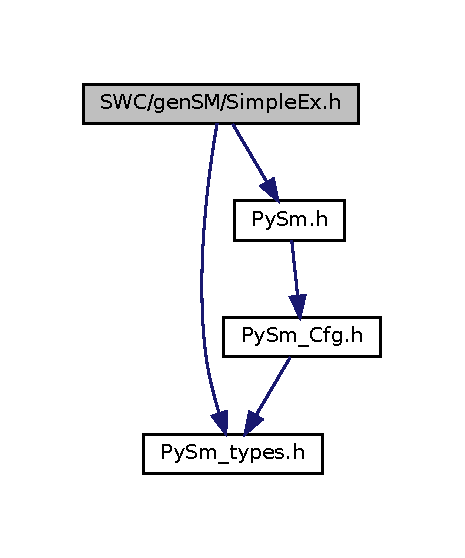
\includegraphics[width=223pt]{SimpleEx_8h__incl}
\end{center}
\end{figure}
This graph shows which files directly or indirectly include this file\+:
\nopagebreak
\begin{figure}[H]
\begin{center}
\leavevmode
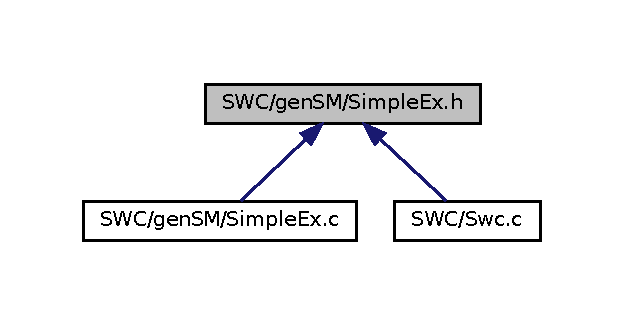
\includegraphics[width=300pt]{SimpleEx_8h__dep__incl}
\end{center}
\end{figure}
\subsection*{Enumerations}
\begin{DoxyCompactItemize}
\item 
enum \hyperlink{SimpleEx_8h_adaa7d471cac739753efb6254f6f039e5}{simple\+Ex\+\_\+active\+State\+Type} \{ \hyperlink{SimpleEx_8h_adaa7d471cac739753efb6254f6f039e5acaffc5763218f7c0b9f77c62754ee635}{S\+I\+M\+P\+L\+E\+E\+X\+\_\+\+U\+N\+I\+N\+I\+T\+A\+L\+I\+Z\+E\+D\+\_\+\+S\+T\+A\+T\+E\+\_\+\+M\+A\+C\+H\+I\+NE}, 
\hyperlink{SimpleEx_8h_adaa7d471cac739753efb6254f6f039e5a71699046bcd083ef741008574b4a61a5}{S\+I\+M\+P\+L\+E\+E\+X\+\_\+state1}, 
\hyperlink{SimpleEx_8h_adaa7d471cac739753efb6254f6f039e5a6bd4a6b22049598434e95c6e68be22a4}{S\+I\+M\+P\+L\+E\+E\+X\+\_\+state2}, 
\hyperlink{SimpleEx_8h_adaa7d471cac739753efb6254f6f039e5a19041f92627883642c2f3909a6af9bdc}{S\+I\+M\+P\+L\+E\+E\+X\+\_\+state3}
 \}\begin{DoxyCompactList}\small\item\em Enum for exporting current active state of state machine simple\+Ex. \end{DoxyCompactList}
\end{DoxyCompactItemize}
\subsection*{Functions}
\begin{DoxyCompactItemize}
\item 
\hyperlink{PySm_8h_a1bd760b7300136bf7e0bd7b9e3a126ff}{py\+Sm\+\_\+return\+Type} \hyperlink{SimpleEx_8h_aa6374857abc588e169064d2f89a0a3e0}{Simple\+Ex\+\_\+main\+Function} (void)
\begin{DoxyCompactList}\small\item\em Main function of the state machine simple\+Ex. \end{DoxyCompactList}\item 
void \hyperlink{SimpleEx_8h_a592039934bbe681d6ee7578ce4b06fa6}{Simple\+Ex\+\_\+get\+Active\+State} (\hyperlink{SimpleEx_8h_adaa7d471cac739753efb6254f6f039e5}{simple\+Ex\+\_\+active\+State\+Type} $\ast$)
\begin{DoxyCompactList}\small\item\em Main function of the state machine simple\+Ex. \end{DoxyCompactList}\end{DoxyCompactItemize}


\subsection{Detailed Description}
Header for generated state machine simple\+Ex Generated 2017-\/11-\/04 13\+:36\+:42 by Py\+SM -\/ The python state machine generator. 

\begin{DoxyAuthor}{Author}
Markus Burger 
\end{DoxyAuthor}
\begin{DoxyDate}{Date}
2017-\/11-\/04 
\end{DoxyDate}


\subsection{Enumeration Type Documentation}
\mbox{\Hypertarget{SimpleEx_8h_adaa7d471cac739753efb6254f6f039e5}\label{SimpleEx_8h_adaa7d471cac739753efb6254f6f039e5}} 
\index{Simple\+Ex.\+h@{Simple\+Ex.\+h}!simple\+Ex\+\_\+active\+State\+Type@{simple\+Ex\+\_\+active\+State\+Type}}
\index{simple\+Ex\+\_\+active\+State\+Type@{simple\+Ex\+\_\+active\+State\+Type}!Simple\+Ex.\+h@{Simple\+Ex.\+h}}
\subsubsection{\texorpdfstring{simple\+Ex\+\_\+active\+State\+Type}{simpleEx\_activeStateType}}
{\footnotesize\ttfamily enum \hyperlink{SimpleEx_8h_adaa7d471cac739753efb6254f6f039e5}{simple\+Ex\+\_\+active\+State\+Type}}



Enum for exporting current active state of state machine simple\+Ex. 

\begin{DoxyEnumFields}{Enumerator}
\raisebox{\heightof{T}}[0pt][0pt]{\index{S\+I\+M\+P\+L\+E\+E\+X\+\_\+\+U\+N\+I\+N\+I\+T\+A\+L\+I\+Z\+E\+D\+\_\+\+S\+T\+A\+T\+E\+\_\+\+M\+A\+C\+H\+I\+NE@{S\+I\+M\+P\+L\+E\+E\+X\+\_\+\+U\+N\+I\+N\+I\+T\+A\+L\+I\+Z\+E\+D\+\_\+\+S\+T\+A\+T\+E\+\_\+\+M\+A\+C\+H\+I\+NE}!Simple\+Ex.\+h@{Simple\+Ex.\+h}}\index{Simple\+Ex.\+h@{Simple\+Ex.\+h}!S\+I\+M\+P\+L\+E\+E\+X\+\_\+\+U\+N\+I\+N\+I\+T\+A\+L\+I\+Z\+E\+D\+\_\+\+S\+T\+A\+T\+E\+\_\+\+M\+A\+C\+H\+I\+NE@{S\+I\+M\+P\+L\+E\+E\+X\+\_\+\+U\+N\+I\+N\+I\+T\+A\+L\+I\+Z\+E\+D\+\_\+\+S\+T\+A\+T\+E\+\_\+\+M\+A\+C\+H\+I\+NE}}}\mbox{\Hypertarget{SimpleEx_8h_adaa7d471cac739753efb6254f6f039e5acaffc5763218f7c0b9f77c62754ee635}\label{SimpleEx_8h_adaa7d471cac739753efb6254f6f039e5acaffc5763218f7c0b9f77c62754ee635}} 
S\+I\+M\+P\+L\+E\+E\+X\+\_\+\+U\+N\+I\+N\+I\+T\+A\+L\+I\+Z\+E\+D\+\_\+\+S\+T\+A\+T\+E\+\_\+\+M\+A\+C\+H\+I\+NE&\\
\hline

\raisebox{\heightof{T}}[0pt][0pt]{\index{S\+I\+M\+P\+L\+E\+E\+X\+\_\+state1@{S\+I\+M\+P\+L\+E\+E\+X\+\_\+state1}!Simple\+Ex.\+h@{Simple\+Ex.\+h}}\index{Simple\+Ex.\+h@{Simple\+Ex.\+h}!S\+I\+M\+P\+L\+E\+E\+X\+\_\+state1@{S\+I\+M\+P\+L\+E\+E\+X\+\_\+state1}}}\mbox{\Hypertarget{SimpleEx_8h_adaa7d471cac739753efb6254f6f039e5a71699046bcd083ef741008574b4a61a5}\label{SimpleEx_8h_adaa7d471cac739753efb6254f6f039e5a71699046bcd083ef741008574b4a61a5}} 
S\+I\+M\+P\+L\+E\+E\+X\+\_\+state1&\\
\hline

\raisebox{\heightof{T}}[0pt][0pt]{\index{S\+I\+M\+P\+L\+E\+E\+X\+\_\+state2@{S\+I\+M\+P\+L\+E\+E\+X\+\_\+state2}!Simple\+Ex.\+h@{Simple\+Ex.\+h}}\index{Simple\+Ex.\+h@{Simple\+Ex.\+h}!S\+I\+M\+P\+L\+E\+E\+X\+\_\+state2@{S\+I\+M\+P\+L\+E\+E\+X\+\_\+state2}}}\mbox{\Hypertarget{SimpleEx_8h_adaa7d471cac739753efb6254f6f039e5a6bd4a6b22049598434e95c6e68be22a4}\label{SimpleEx_8h_adaa7d471cac739753efb6254f6f039e5a6bd4a6b22049598434e95c6e68be22a4}} 
S\+I\+M\+P\+L\+E\+E\+X\+\_\+state2&\\
\hline

\raisebox{\heightof{T}}[0pt][0pt]{\index{S\+I\+M\+P\+L\+E\+E\+X\+\_\+state3@{S\+I\+M\+P\+L\+E\+E\+X\+\_\+state3}!Simple\+Ex.\+h@{Simple\+Ex.\+h}}\index{Simple\+Ex.\+h@{Simple\+Ex.\+h}!S\+I\+M\+P\+L\+E\+E\+X\+\_\+state3@{S\+I\+M\+P\+L\+E\+E\+X\+\_\+state3}}}\mbox{\Hypertarget{SimpleEx_8h_adaa7d471cac739753efb6254f6f039e5a19041f92627883642c2f3909a6af9bdc}\label{SimpleEx_8h_adaa7d471cac739753efb6254f6f039e5a19041f92627883642c2f3909a6af9bdc}} 
S\+I\+M\+P\+L\+E\+E\+X\+\_\+state3&\\
\hline

\end{DoxyEnumFields}


\subsection{Function Documentation}
\mbox{\Hypertarget{SimpleEx_8h_a592039934bbe681d6ee7578ce4b06fa6}\label{SimpleEx_8h_a592039934bbe681d6ee7578ce4b06fa6}} 
\index{Simple\+Ex.\+h@{Simple\+Ex.\+h}!Simple\+Ex\+\_\+get\+Active\+State@{Simple\+Ex\+\_\+get\+Active\+State}}
\index{Simple\+Ex\+\_\+get\+Active\+State@{Simple\+Ex\+\_\+get\+Active\+State}!Simple\+Ex.\+h@{Simple\+Ex.\+h}}
\subsubsection{\texorpdfstring{Simple\+Ex\+\_\+get\+Active\+State()}{SimpleEx\_getActiveState()}}
{\footnotesize\ttfamily void Simple\+Ex\+\_\+get\+Active\+State (\begin{DoxyParamCaption}\item[{\hyperlink{SimpleEx_8h_adaa7d471cac739753efb6254f6f039e5}{simple\+Ex\+\_\+active\+State\+Type} $\ast$}]{ }\end{DoxyParamCaption})}



Main function of the state machine simple\+Ex. 

\mbox{\Hypertarget{SimpleEx_8h_aa6374857abc588e169064d2f89a0a3e0}\label{SimpleEx_8h_aa6374857abc588e169064d2f89a0a3e0}} 
\index{Simple\+Ex.\+h@{Simple\+Ex.\+h}!Simple\+Ex\+\_\+main\+Function@{Simple\+Ex\+\_\+main\+Function}}
\index{Simple\+Ex\+\_\+main\+Function@{Simple\+Ex\+\_\+main\+Function}!Simple\+Ex.\+h@{Simple\+Ex.\+h}}
\subsubsection{\texorpdfstring{Simple\+Ex\+\_\+main\+Function()}{SimpleEx\_mainFunction()}}
{\footnotesize\ttfamily \hyperlink{PySm_8h_a1bd760b7300136bf7e0bd7b9e3a126ff}{py\+Sm\+\_\+return\+Type} Simple\+Ex\+\_\+main\+Function (\begin{DoxyParamCaption}\item[{void}]{ }\end{DoxyParamCaption})}



Main function of the state machine simple\+Ex. 

Here is the call graph for this function\+:
\nopagebreak
\begin{figure}[H]
\begin{center}
\leavevmode
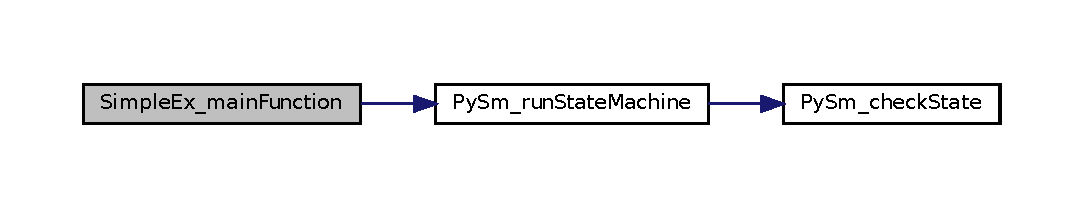
\includegraphics[width=350pt]{SimpleEx_8h_aa6374857abc588e169064d2f89a0a3e0_cgraph}
\end{center}
\end{figure}

\hypertarget{Swc_8c}{}\section{S\+W\+C/\+Swc.c File Reference}
\label{Swc_8c}\index{S\+W\+C/\+Swc.\+c@{S\+W\+C/\+Swc.\+c}}


Test-\/\+S\+WC to demonstrate the use of the generated state machine.  


{\ttfamily \#include \char`\"{}Swc.\+h\char`\"{}}\newline
{\ttfamily \#include \char`\"{}Dev\+Coffee.\+h\char`\"{}}\newline
{\ttfamily \#include $<$stdint.\+h$>$}\newline
Include dependency graph for Swc.\+c\+:
\nopagebreak
\begin{figure}[H]
\begin{center}
\leavevmode
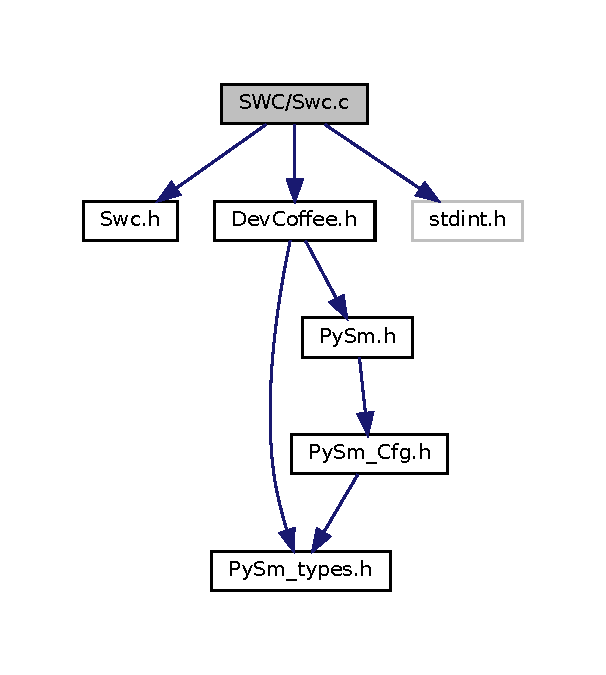
\includegraphics[width=291pt]{Swc_8c__incl}
\end{center}
\end{figure}
\subsection*{Functions}
\begin{DoxyCompactItemize}
\item 
void \hyperlink{Swc_8c_a5799359ce667341ad4694a6ceb9ae96b}{Swc\+\_\+main} (void)
\end{DoxyCompactItemize}


\subsection{Detailed Description}
Test-\/\+S\+WC to demonstrate the use of the generated state machine. 

\begin{DoxyAuthor}{Author}
Markus Burger 
\end{DoxyAuthor}
\begin{DoxyDate}{Date}
2017-\/09-\/11 
\end{DoxyDate}


\subsection{Function Documentation}
\mbox{\Hypertarget{Swc_8c_a5799359ce667341ad4694a6ceb9ae96b}\label{Swc_8c_a5799359ce667341ad4694a6ceb9ae96b}} 
\index{Swc.\+c@{Swc.\+c}!Swc\+\_\+main@{Swc\+\_\+main}}
\index{Swc\+\_\+main@{Swc\+\_\+main}!Swc.\+c@{Swc.\+c}}
\subsubsection{\texorpdfstring{Swc\+\_\+main()}{Swc\_main()}}
{\footnotesize\ttfamily void Swc\+\_\+main (\begin{DoxyParamCaption}\item[{void}]{ }\end{DoxyParamCaption})}

Here is the call graph for this function\+:\nopagebreak
\begin{figure}[H]
\begin{center}
\leavevmode
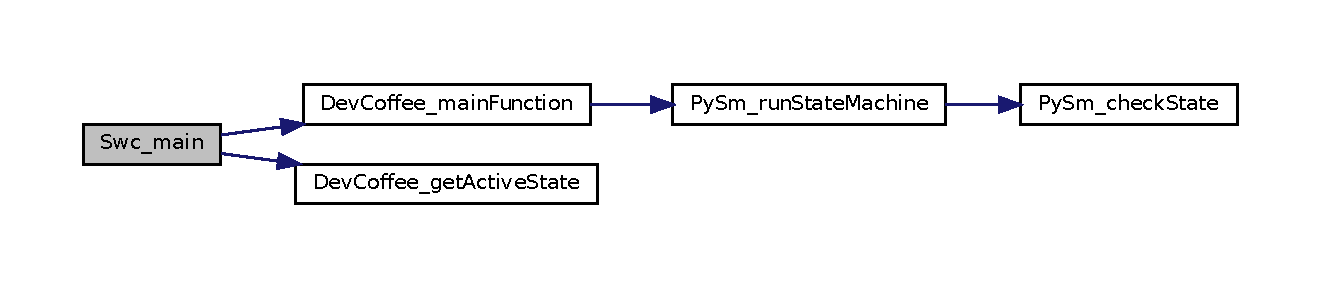
\includegraphics[width=350pt]{Swc_8c_a5799359ce667341ad4694a6ceb9ae96b_cgraph}
\end{center}
\end{figure}

\hypertarget{Swc_8h}{}\section{S\+W\+C/\+Swc.h File Reference}
\label{Swc_8h}\index{S\+W\+C/\+Swc.\+h@{S\+W\+C/\+Swc.\+h}}


Header file of Test-\/\+S\+WC to demonstrate the use of the generated state machine.  


This graph shows which files directly or indirectly include this file\+:\nopagebreak
\begin{figure}[H]
\begin{center}
\leavevmode
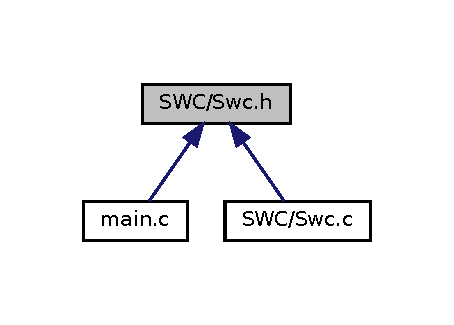
\includegraphics[width=218pt]{Swc_8h__dep__incl}
\end{center}
\end{figure}
\subsection*{Functions}
\begin{DoxyCompactItemize}
\item 
void \hyperlink{Swc_8h_a5799359ce667341ad4694a6ceb9ae96b}{Swc\+\_\+main} (void)
\end{DoxyCompactItemize}


\subsection{Detailed Description}
Header file of Test-\/\+S\+WC to demonstrate the use of the generated state machine. 

\begin{DoxyAuthor}{Author}
Markus Burger 
\end{DoxyAuthor}
\begin{DoxyDate}{Date}
2017-\/09-\/11 
\end{DoxyDate}


\subsection{Function Documentation}
\mbox{\Hypertarget{Swc_8h_a5799359ce667341ad4694a6ceb9ae96b}\label{Swc_8h_a5799359ce667341ad4694a6ceb9ae96b}} 
\index{Swc.\+h@{Swc.\+h}!Swc\+\_\+main@{Swc\+\_\+main}}
\index{Swc\+\_\+main@{Swc\+\_\+main}!Swc.\+h@{Swc.\+h}}
\subsubsection{\texorpdfstring{Swc\+\_\+main()}{Swc\_main()}}
{\footnotesize\ttfamily void Swc\+\_\+main (\begin{DoxyParamCaption}\item[{void}]{ }\end{DoxyParamCaption})}

Here is the call graph for this function\+:
\nopagebreak
\begin{figure}[H]
\begin{center}
\leavevmode
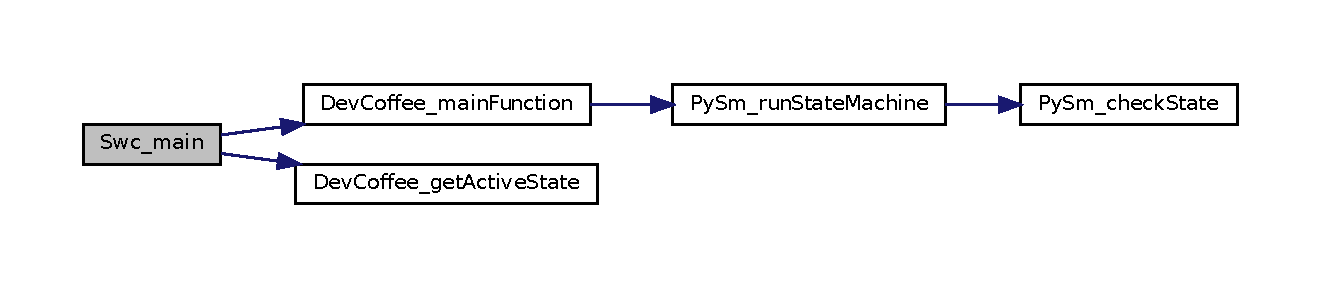
\includegraphics[width=350pt]{Swc_8h_a5799359ce667341ad4694a6ceb9ae96b_cgraph}
\end{center}
\end{figure}

%--- End generated contents ---

% Index
\backmatter
\newpage
\phantomsection
\clearemptydoublepage
\addcontentsline{toc}{chapter}{Index}
\printindex

\end{document}
